\documentclass[12pt,a4paper,oneside]{report}

\usepackage{cmap}
\usepackage[utf8]{inputenc}
\usepackage[T1]{fontenc}
\usepackage[brazil,english]{babel}
\usepackage{geometry}
\usepackage{graphicx}
\usepackage{booktabs}
\usepackage{array}
\usepackage{longtable}
\usepackage{tabularx}
\usepackage{ragged2e}
\usepackage{makecell}
\usepackage{pdflscape}
\usepackage{seqsplit}
\usepackage{xcolor}
\usepackage{hyperref}
\usepackage{amsmath}
\usepackage{amssymb}
\usepackage{caption}
\usepackage{float}
\usepackage{fancyhdr}
\usepackage{setspace}
\usepackage{lmodern}
\usepackage{microtype}
\usepackage{csquotes}
\usepackage{siunitx}
\usepackage[backend=biber,style=numeric,sorting=none]{biblatex}

\AtEveryBibitem{%
  \clearfield{note}%
  \clearfield{file}%
}
\addbibresource{../references.bib}

\geometry{margin=2.5cm}
\onehalfspacing
\setlength{\emergencystretch}{2em}
\sisetup{locale=DE}

\definecolor{clblue}{RGB}{32,68,112}
\definecolor{clgray}{RGB}{245,247,250}

\hypersetup{
  colorlinks=true,
  linkcolor=clblue,
  citecolor=clblue,
  urlcolor=clblue,
  pdftitle={CabotageLens: Relatorio final de TF},
  pdfauthor={Felipe de Sá Proença}
}

\pagestyle{fancy}
\fancyhf{}
\lhead{\nouppercase{\leftmark}}
\rhead{\thepage}
\setlength{\headheight}{15pt}

\newcommand{\CabotageLens}{\textit{CabotageLens}}
\newcommand{\cooe}{CO$_2$e}
\newcommand{\ttw}{TTW}
\newcommand{\wtw}{WTW}
\newcolumntype{Y}{>{\RaggedRight\arraybackslash}X}
\newcolumntype{L}[1]{>{\RaggedRight\arraybackslash}p{#1}}
\newcommand{\codecell}[1]{\texttt{\seqsplit{#1}}}
\newcommand{\methodnote}[1]{%
  \begin{center}
  \fcolorbox{clblue}{clgray}{%
    \parbox{0.90\textwidth}{\small #1}%
  }
  \end{center}
}
\newcommand{\reporttitle}{CabotageLens: framework computacional auditável para comparação porta a porta entre rodovia e cabotagem no Brasil}
\newcommand{\reportauthor}{Felipe de Sá Proença}
\newcommand{\reportadvisor}{Prof. Dr. Marcos Mendes de Oliveira Pinto}
\newcommand{\reportinstitution}{Escola Politécnica da Universidade de São Paulo}
\newcommand{\reportcourse}{Engenharia Naval}
\newcommand{\reportlocation}{São Paulo}
\newcommand{\reportyear}{2026}

\begin{document}

\selectlanguage{brazil}

\begin{titlepage}
\centering
{\large \reportinstitution\par}
\vspace{0.5cm}
{\large \reportcourse\par}
\vfill
{\Large\bfseries \reporttitle\par}
\vspace{1.5cm}
{\large \reportauthor\par}
\vfill
\begin{flushleft}
\textbf{Orientador(a):} \reportadvisor\\
\textbf{Local:} \reportlocation\\
\textbf{Ano:} \reportyear
\end{flushleft}
\vspace{1cm}
{\reportlocation\\\reportyear\par}
\end{titlepage}

\pagenumbering{roman}

\chapter*{Resumo}
\markboth{Resumo}{Resumo}
\addcontentsline{toc}{chapter}{Resumo}
Este relatório explica o funcionamento do \CabotageLens{}, uma ferramenta computacional criada para comparar duas formas de transportar a mesma carga entre a mesma origem e o mesmo destino. A primeira alternativa usa somente rodovia. A segunda combina acesso rodoviário ao porto, navegação por cabotagem e acesso rodoviário ao destino final. O sistema calcula cada parte da viagem separadamente e informa de onde vieram as distâncias, os fatores de consumo e os demais parâmetros.

O cálculo marítimo combina as tabelas de Carga e Atracação da ANTAQ com os indicadores do EU MRV. Para cada par de portos, entram todas as viagens em que a origem aparece antes do destino. Isso inclui viagens diretas e viagens com escalas intermediárias. Em cada viagem, o sistema reconstrói a carga que estava a bordo e soma o consumo de todos os subtrechos. A intensidade do navio é procurada primeiro pelo número IMO. Quando não existe correspondência no EU MRV, o sistema usa uma estatística robusta da classe ou do tipo do navio e registra esse fallback como uma aproximação. A intensidade final do par é uma mediana ponderada pelo trabalho de transporte. A escolha do corredor é feita separadamente e fornece apenas a sequência de portos e a distância usada no cenário.

A matriz resultante contém 177 pares direcionais, 12.025 observações viagem--OD e 5.438 subtrechos. Desses subtrechos, 3.290 usam intensidade obtida por IMO e 2.148 usam fallback. O par Santos--Manaus mostra como interpretar o resultado: 89 viagens, distribuídas em 22 corredores, formam a amostra estatística; a intensidade representativa é 9,322050 g/(t$\cdot$nm); e a ligação direta de 6.112 km fornece a geometria. Em uma remessa hipotética de 14 t, essa intensidade e a distância de 3.300,216 milhas náuticas correspondem a 430,71 kg de combustível apenas para a navegação. A comparação externa é usada somente como verificação direcional. Os resultados não representam frete comercial, garantia de serviço, avaliação \wtw{}/LCA ou superioridade universal da cabotagem.

\textbf{Palavras-chave}: cabotagem; transporte rodoviário; transporte multimodal; emissões operacionais; \cooe{}; custo modelado; rastreabilidade; Brasil.

\chapter*{Abstract}
\markboth{Abstract}{Abstract}
\addcontentsline{toc}{chapter}{Abstract}
\selectlanguage{english}
This report explains \CabotageLens{}, a computational tool that compares two ways of moving the same cargo between the same origin and destination. The first alternative uses road transport only. The second combines road access to the departure port, coastal shipping, and road access from the arrival port to the final destination. Each leg is calculated separately, and the system records the source of distances, fuel-intensity values, and other parameters.

The maritime calculation combines ANTAQ Cargo and Port Call tables with EU MRV indicators. For each port pair, it includes every voyage in which the origin appears before the destination, including direct and multi-stop voyages. The system reconstructs onboard cargo and sums the consumption of all sublegs. Vessel intensity is searched first by IMO number. If no EU MRV match exists, a robust vessel-class or ship-type statistic is used and explicitly recorded as a fallback. The final OD intensity is a transport-work-weighted median. Corridor selection is separate and supplies only the port sequence and distance used in the scenario.

The matrix contains 177 directional pairs, 12,025 voyage--OD observations, and 5,438 sublegs. Of these sublegs, 3,290 use IMO-matched intensity and 2,148 use a fallback. Santos--Manaus provides a concrete reading example: 89 voyages across 22 corridors form the statistical sample, the representative intensity is 9.322050 g/(t$\cdot$nm), and the direct 6,112 km connection supplies the geometry. For a hypothetical 14 t shipment, that intensity and the 3,300.216 nautical-mile distance correspond to 430.71 kg of navigation fuel only. The external comparison is used as directional evidence. Results are not commercial freight quotations, service guarantees, WTW/LCA assessments, or proof of universal modal superiority.

\textbf{Keywords}: coastal shipping; road freight; multimodal freight; operational emissions; \cooe{}; modeled cost; traceability; Brazil.
\selectlanguage{brazil}

\markboth{Sumário}{Sumário}
\tableofcontents
\markboth{Lista de Figuras}{Lista de Figuras}
\listoffigures
\markboth{Lista de Tabelas}{Lista de Tabelas}
\listoftables

\cleardoublepage
\chapter*{Dicionário de termos, siglas e abreviações}
\markboth{Dicionário de termos, siglas e abreviações}{Dicionário de termos, siglas e abreviações}
\phantomsection
\addcontentsline{toc}{chapter}{Dicionário de termos, siglas e abreviações}
\small
\begin{description}
  \item[ANTAQ] Agência Nacional de Transportes Aquaviários.
  \item[EU MRV] Sistema europeu de monitoramento, reporte e verificação de emissões e atividade de navios.
  \item[IMO] Número permanente de identificação internacional da embarcação.
  \item[OD] Par origem-destino usado para definir a remessa ou o corredor analisado.
  \item[TEU] Unidade equivalente a contêiner de 20 pés.
  \item[BRL] Real brasileiro, unidade monetária usada para expressar o proxy de custo operacional modelado.
  \item[BR do Mar] Programa brasileiro associado ao transporte marítimo costeiro.
  \item[SSS] \textit{Short sea shipping}, transporte marítimo de curta distância ou costeiro.
  \item[Transporte rodoviário direto] Alternativa formada por uma perna rodoviária entre origem e destino.
  \item[Alternativa multimodal] Cadeia com acesso rodoviário inicial, perna marítima, portos e acesso rodoviário final.
  \item[Pre-carriage] Trecho rodoviário inicial entre a origem da carga e o porto de embarque.
  \item[On-carriage] Trecho rodoviário final entre o porto de desembarque e o destino da carga.
  \item[Operações portuárias] Atividades realizadas em porto ou terminal para atendimento da carga e da embarcação.
  \item[Hoteling/hotelling] Permanência do navio atracado ou em porto, com consumo de energia para sistemas de bordo.
  \item[\ttw{}] Fronteira operacional \textit{tank-to-wheel}/\textit{tank-to-wake}.
  \item[\wtw{}] Perspectiva \textit{well-to-wheel}/\textit{well-to-wake}.
  \item[LCA/ACV] Avaliação de ciclo de vida.
  \item[CO$_2$] Dióxido de carbono.
  \item[\cooe{}] Dióxido de carbono equivalente.
  \item[CO$_2$eq] Notação para dióxido de carbono equivalente em fontes ou benchmarks externos.
  \item[GEE/GHG] Gases de efeito estufa.
  \item[Unidade funcional] Base comum usada para comparar alternativas de transporte.
  \item[Carga útil] Massa de carga efetivamente transportada na remessa ou cenário.
  \item[Viagem--OD] Observação formada quando o porto de origem precede o porto de destino na sequência da mesma viagem.
  \item[Corredor observado] Sequência de portos percorrida entre a origem e o destino em uma viagem ANTAQ.
  \item[Subtrecho] Perna navegada entre duas escalas consecutivas, com distância e carga a bordo associadas.
  \item[Carga a bordo] Massa reconstruída que o navio transporta ao sair de uma escala e durante o subtrecho seguinte.
  \item[Intensidade marítima] Quantidade de combustível associada a uma tonelada de carga transportada por uma milha náutica, expressa em g/(t$\cdot$nm).
  \item[Trabalho de transporte] Produto entre massa transportada e distância, expresso neste estudo em t$\cdot$nm.
  \item[Mediana ponderada] Primeiro valor ordenado cuja soma acumulada dos pesos alcança 50\% do peso total.
  \item[Média aparada] Média calculada após a retirada simétrica de uma fração das menores e maiores observações.
  \item[Fator de emissão] Coeficiente que relaciona consumo, energia ou atividade a emissões.
  \item[Proxy de custo operacional modelado] Estimativa monetária parcial calculada para os componentes representados.
  \item[Frete comercial] Preço de mercado negociado, cotado ou contratado para transporte.
  \item[Fallback] Aproximação ou fonte alternativa usada quando não há dado mais forte.
  \item[Proveniência] Registro da origem e confiabilidade de um dado.
  \item[Benchmark] Referência externa usada para comparação ou plausibilidade.
  \item[Evidência direcional] Evidência de que duas fontes ou execuções apontam o mesmo sentido de resultado.
  \item[Classificação conservadora] Categoria de uso atribuída à evidência para limitar sua interpretação.
  \item[Análise de sensibilidade] Execução sob hipótese documentada para avaliar dependência do resultado.
  \item[Reprodutibilidade] Capacidade de rastrear e repetir entradas, parâmetros, resultados e classificações.
\end{description}
\normalsize
\clearpage
\pagenumbering{arabic}

\chapter{Introdução}
\label{ch:introducao}

O transporte de cargas no Brasil depende fortemente das rodovias. O caminhão oferece capilaridade e permite o atendimento porta a porta. Em viagens longas, porém, essa escolha também concentra consumo de diesel, custo operacional e emissões.

A cabotagem é a navegação entre portos do mesmo país. Ela pode substituir parte do percurso rodoviário quando a origem e o destino podem ser ligados por três etapas: acesso rodoviário ao porto, navegação costeira e acesso rodoviário ao destino final \cite{icct2022}. Portanto, a cabotagem não elimina necessariamente o caminhão. Ela muda a função do transporte rodoviário dentro da cadeia.

Um exemplo ajuda a visualizar o problema. Para transportar uma remessa de São Paulo a Manaus, a alternativa rodoviária direta liga as duas cidades por estrada. Uma alternativa multimodal pode levar a carga por rodovia até Santos, transportá-la por navio até Manaus e completar por rodovia o acesso ao destino. A comparação correta deve incluir todas essas etapas. Comparar apenas o navio com o caminhão produziria uma fronteira incompleta.

Neste relatório, o acesso inicial ao porto é chamado de \emph{pre-carriage}. O acesso final, entre o porto de destino e o destino da carga, é chamado de \emph{on-carriage}. A cadeia também pode conter operações portuárias e \emph{hoteling}, isto é, a permanência do navio no porto com sistemas de bordo em funcionamento. A conclusão depende das distâncias de cada trecho, dos portos escolhidos, das fontes dessas distâncias, da carga, do consumo, da alocação e da fronteira metodológica \cite{shortsea2019,modalshiftreview2020}.

\begin{figure}[htbp]
\centering
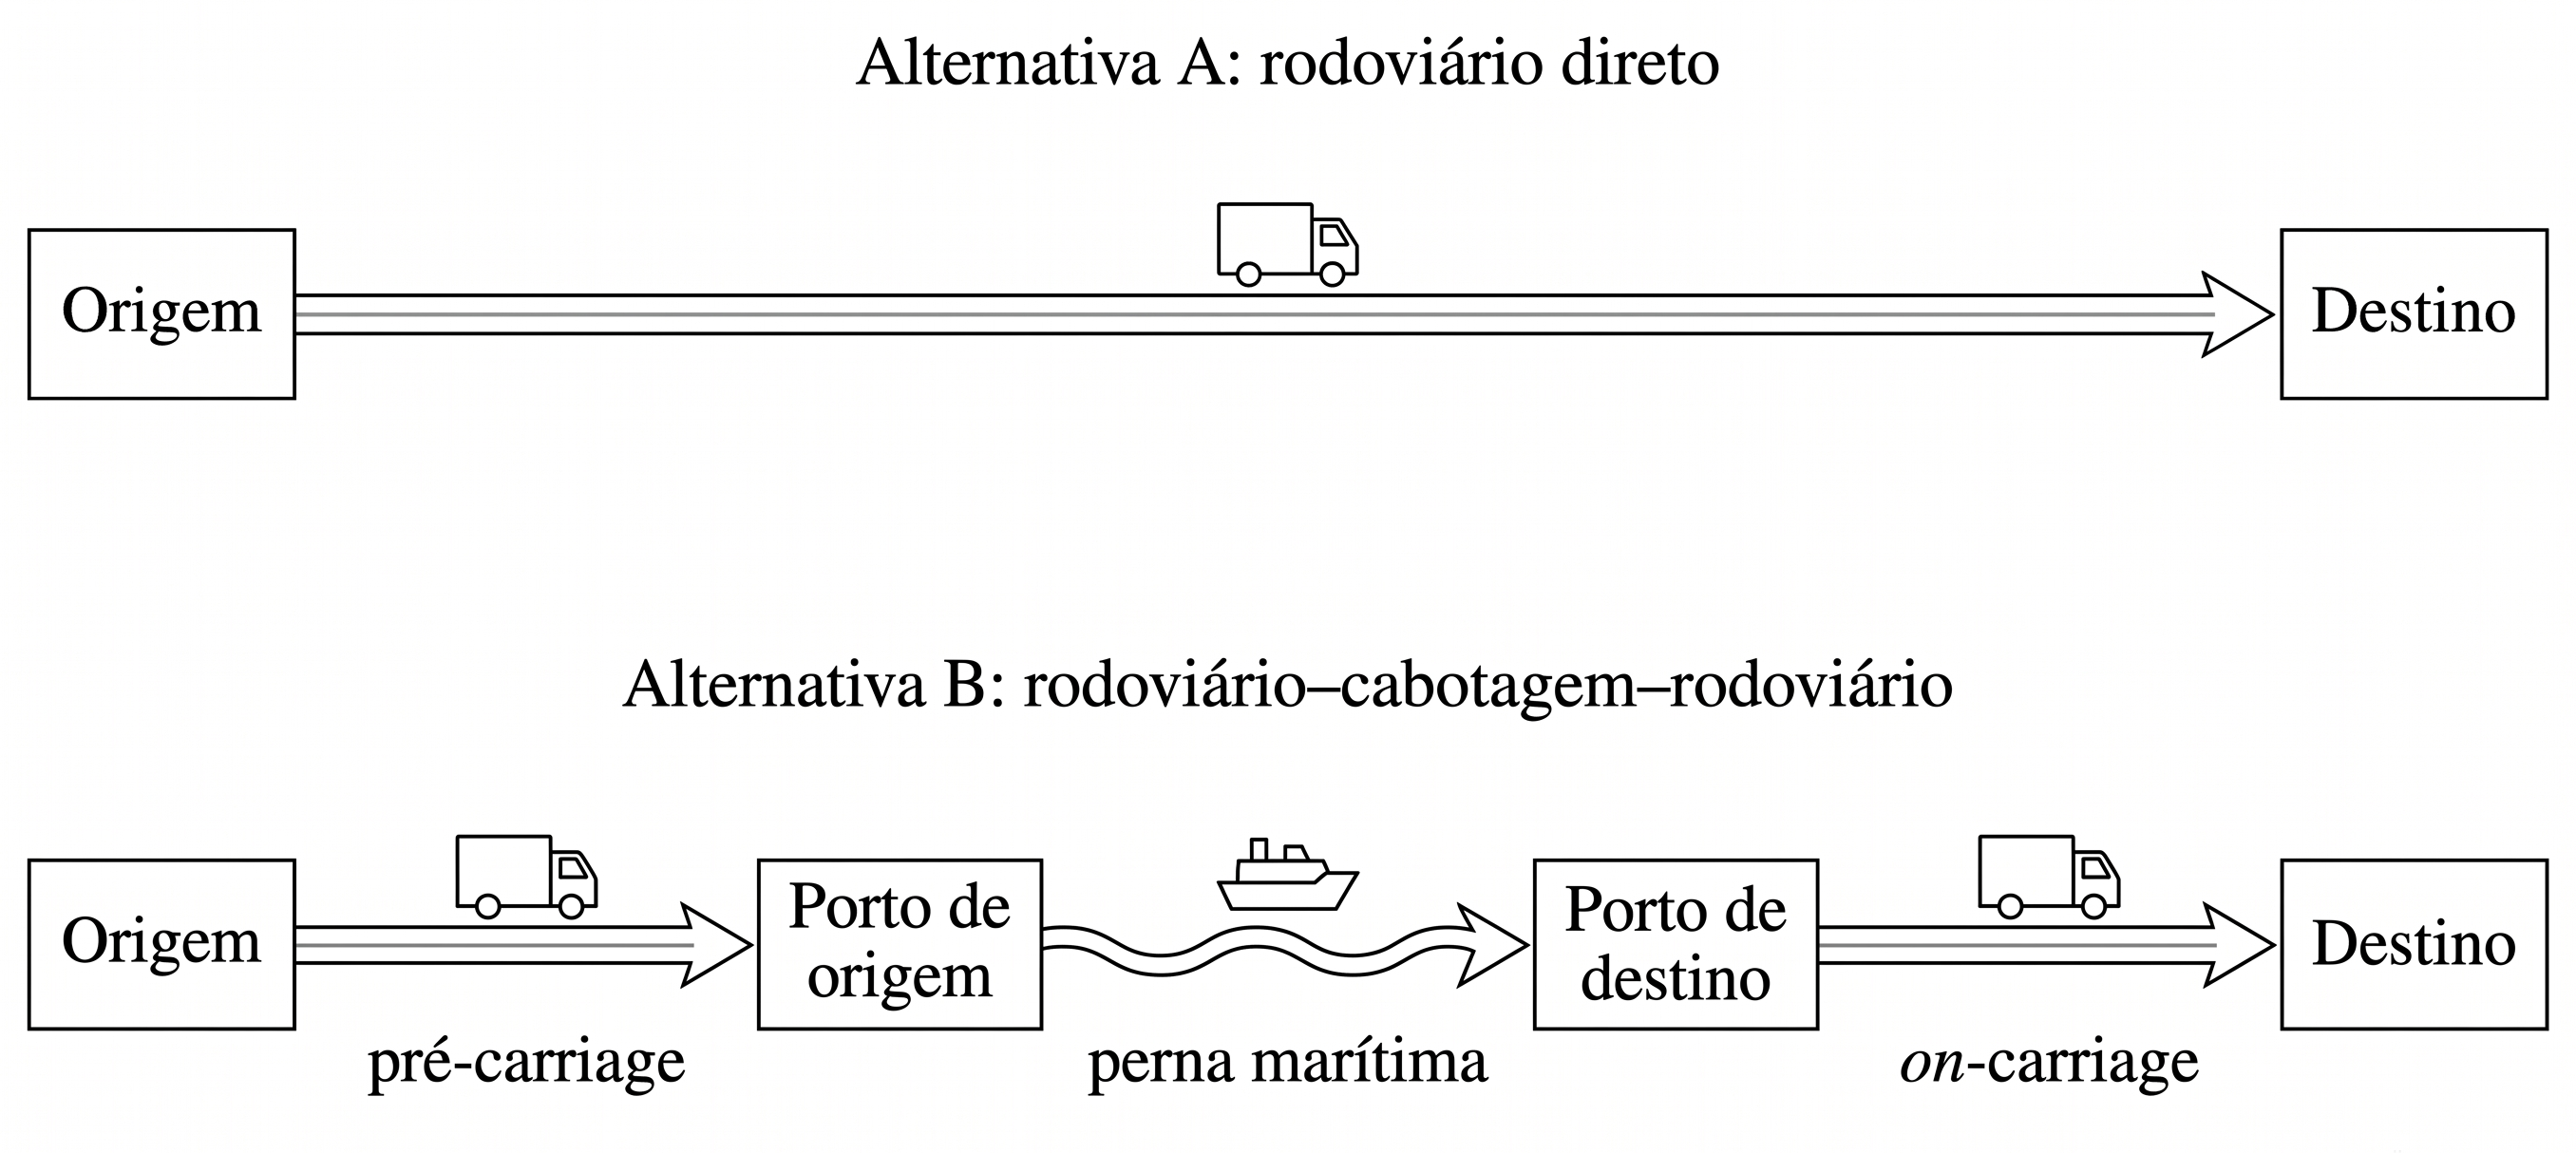
\includegraphics[width=0.95\textwidth]{images/figura_1_1.png}
\caption{Comparação conceitual entre a alternativa rodoviária direta e a cadeia multimodal rodoviária--cabotagem--rodoviária, avaliadas sob a mesma unidade funcional e fronteira porta a porta.}
\label{fig:comparacao-porta-a-porta}
\end{figure}

A Figura~\ref{fig:comparacao-porta-a-porta} resume as duas alternativas. Em ambas, a entrada principal é a mesma remessa, com a mesma origem e o mesmo destino. O processamento muda conforme a cadeia escolhida. A saída reúne distância, consumo, custo modelado e emissões operacionais para cada alternativa.

Decisões logísticas reais também envolvem frequência de serviço, disponibilidade de navios, terminais, tempo de trânsito, confiabilidade, escala, custos comerciais e estrutura de rede \cite{competitiveness2024,modalshiftreview2020}. O escopo deste trabalho é mais específico. Ele constrói uma comparação computacional e rastreável entre a rota rodoviária direta e a cadeia rodoviária--cabotagem--rodoviária. A ferramenta não confirma contratação, frequência ou disponibilidade comercial.

A contribuição central é o \CabotageLens{}. Trata-se de um framework computacional e de um protótipo auditável para comparação acadêmica de alternativas de transporte. Para cada cenário, a ferramenta organiza três grupos de informação:

\begin{itemize}
  \item \textbf{Entradas:} origem, destino, massa da carga, portos e parâmetros técnicos.
  \item \textbf{Processamento:} resolução das rotas, construção das pernas logísticas e cálculo de combustível, custo modelado e emissões.
  \item \textbf{Saídas:} resultados por perna, totais das duas alternativas, fontes utilizadas e avisos de qualidade.
\end{itemize}

Na perna marítima, o método combina as tabelas de Carga e Atracação da ANTAQ com os indicadores de eficiência do EU MRV. Primeiro, o sistema ordena as escalas de cada viagem. Depois, identifica todos os casos em que o porto de origem aparece antes do porto de destino. Uma viagem direta e outra com escalas intermediárias são válidas, desde que respeitem essa ordem.

Em seguida, a carga a bordo é reconstruída em cada subtrecho. O trabalho de transporte da viagem é calculado com a carga e a distância de cada trecho. A intensidade do navio é procurada pelo número IMO no EU MRV. Quando não há correspondência, usa-se uma estatística robusta da classe ou do tipo de embarcação. A fonte escolhida acompanha o resultado. Por fim, a intensidade representativa do par de portos é obtida pela mediana das intensidades das viagens elegíveis, ponderada pelo trabalho de transporte.

O protótipo prioriza recursos computacionais acessíveis. Quando aplicável, utiliza bibliotecas de código aberto e serviços públicos, gratuitos ou com camada gratuita. Essa escolha facilita a reprodução acadêmica e a inspeção dos cálculos. Ela não representa, entretanto, uma garantia de que provedores externos permanecerão gratuitos ou disponíveis.

\methodnote{\textbf{Como ler a fronteira do trabalho.} A saída ambiental representa emissões operacionais \ttw{} de \cooe{}. A saída econômica é um proxy de custo operacional modelado. Ela não é uma cotação de frete.}

Operações portuárias e \emph{hoteling} seguem a fronteira do indicador marítimo utilizado. As operações portuárias permanecem explícitas quando há proveniência documentada. Quando se aplica a intensidade marítima por trabalho de transporte do MRV, o consumo anual reportado do navio é tratado como abrangente para essa finalidade. Nesse caso, o \emph{hoteling} não é somado separadamente, evitando dupla contagem. Se um dado não estiver disponível, o sistema o identifica como indisponível; ele não o transforma em zero.

Assim, o resultado do \CabotageLens{} deve ser lido junto com suas entradas, fontes e limites. A ferramenta mostra quando a alternativa multimodal é promissora dentro da fronteira avaliada. Também mostra quais lacunas impedem uma conclusão mais forte. Essa rastreabilidade é parte do método, e não apenas uma informação adicional.

\chapter{Objetivos}
\label{ch:objetivos}

\section{Objetivo geral}
\label{sec:objetivo-geral}

Desenvolver, implementar e documentar o \CabotageLens{} como um framework computacional auditável para comparar o transporte rodoviário direto com uma cadeia rodoviária--cabotagem--rodoviária em corredores brasileiros, considerando emissões operacionais \ttw{} de \cooe{} e proxy de custo operacional modelado sob fronteiras metodológicas explícitas.

\section{Objetivos específicos}
\label{sec:objetivos-especificos}

Os objetivos específicos do trabalho são:

\begin{itemize}
  \item Definir a unidade funcional do estudo e as alternativas comparáveis como cadeias porta a porta, distinguindo a rota rodoviária direta da cadeia rodoviária--cabotagem--rodoviária.
  \item Construir alternativas orientadas por rota para pares origem-destino selecionados, incluindo acesso rodoviário inicial, perna marítima, operações portuárias e \emph{hoteling} quando aplicáveis, e acesso rodoviário final.
  \item Reconstruir as viagens de cabotagem observadas nas tabelas de Carga e Atracação da ANTAQ, preservando a ordem das escalas, os embarques e desembarques e a carga a bordo em cada subtrecho.
  \item Considerar, para cada par portuário direcionado, todas as viagens em que a origem antecede o destino, incluindo ligações diretas, escalas intermediárias e corredores distintos observados na base.
  \item Associar as viagens aos indicadores de intensidade por trabalho de transporte do EU MRV por meio do número IMO e resolver ausências com estatística robusta de classe ou tipo de navio, registrando a origem de cada valor.
  \item Estimar a intensidade marítima representativa de cada par origem--destino pela mediana ponderada pelo trabalho de transporte das viagens elegíveis, mantendo a escolha do corredor físico separada da agregação estatística da intensidade.
  \item Preservar a proveniência de distâncias, seleção de portos, construção da perna marítima e insumos de operações portuárias/\emph{hoteling}, incluindo níveis de fonte, \emph{fallbacks}, avisos e dados indisponíveis.
  \item Estimar, para os cenários selecionados, emissões operacionais \ttw{} de \cooe{} e proxy de custo operacional modelado, mantendo unidades, fronteiras e limites de interpretação explícitos.
  \item Expor hipóteses, aproximações, avisos de rota, lacunas de dados e componentes indisponíveis, evitando que ausência de informação seja interpretada como valor nulo.
  \item Documentar a implementação computacional com ênfase em rastreabilidade, reprodutibilidade e recursos acessíveis, priorizando bibliotecas de código aberto e serviços públicos, gratuitos ou com camada gratuita quando aplicável, de modo a facilitar auditoria, inspeção e extensão futura do protótipo.
  \item Classificar os resultados de forma conservadora segundo qualidade da evidência, sensibilidade a premissas, limitações de rota e comparabilidade externa.
  \item Usar análises de sensibilidade e evidência externa de benchmark para apoiar interpretação acadêmica defensável, sem afirmar equivalência calibrada de magnitude.
  \item Discutir limitações e melhorias futuras para o uso metodológico, acadêmico e computacional do \CabotageLens{}.
\end{itemize}

Esses objetivos delimitam a leitura do relatório. O trabalho promete uma comparação auditável e condicionada por fronteiras explícitas; não promete resolver contratação comercial, disponibilidade operacional, preço de mercado, super-rede multimodal completa ou superioridade universal da cabotagem.

\chapter{Revisão bibliográfica}
\label{ch:revisao}

Este capítulo apresenta os conceitos necessários para compreender o \CabotageLens{}. A revisão segue uma pergunta simples: o que precisa ser considerado para comparar, de forma justa, uma rota rodoviária direta com uma cadeia que utiliza cabotagem?

A resposta é construída em etapas. Primeiro, apresenta-se o contexto brasileiro. Depois, discutem-se mudança modal e comparação porta a porta. Em seguida, são explicadas as fontes ANTAQ e EU MRV, as fronteiras ambientais, as operações portuárias e a fronteira econômica. A literatura fornece o fundamento conceitual. Os resultados numéricos permanecem vinculados aos artefatos rastreados do projeto.

\section{Cabotagem brasileira, matriz de transporte e BR do Mar}
\label{sec:cabotagem-br}

Cabotagem é o transporte marítimo entre portos de um mesmo país. No Brasil, ela é relevante porque o território possui longas distâncias internas, extensa costa e forte dependência do transporte rodoviário. A agenda associada ao BR do Mar faz parte da discussão sobre diversificação da matriz de transporte e descarbonização dos corredores de carga \cite{icct2022}.

Esse contexto explica por que a cabotagem merece ser estudada. Ele não determina, por si só, que ela será melhor em toda rota. Por exemplo, uma origem distante de qualquer porto pode exigir um acesso rodoviário longo. Esse acesso pode reduzir parte do benefício esperado da navegação.

Portanto, o problema deve ser analisado rota a rota. As entradas relevantes são a origem, o destino, a carga e os portos. O processamento precisa incluir as distâncias terrestres e marítimas. A saída só é interpretável quando a unidade funcional e as fronteiras ambiental e econômica permanecem iguais nas alternativas comparadas.

\section{Mudança modal e short sea shipping}
\label{sec:sss-modal-shift}

Mudança modal é a transferência de uma carga de um modo de transporte para outro. No contexto deste trabalho, significa substituir parte de um percurso rodoviário por navegação costeira, sem deixar de considerar os acessos terrestres.

Revisões sobre \emph{short sea shipping}, ou navegação marítima de curta distância, mostram que essa transferência depende de custo, tempo, confiabilidade, integração terrestre, qualidade de serviço, características portuárias e barreiras institucionais \cite{modalshiftreview2020}. Estudos de emissões também indicam que o resultado varia com o corredor, a utilização e o tipo do navio, a distância, os acessos terrestres e as premissas de cálculo \cite{shortsea2019}.

A consequência para o \CabotageLens{} é direta. A pergunta não é ``o navio emite menos que o caminhão?''. A pergunta é: ``para esta remessa, nesta origem e neste destino, a cadeia completa com cabotagem apresenta melhor resultado que a rota rodoviária direta?''. A resposta vale para o cenário calculado e não para todos os corredores brasileiros.

\section{Comparações porta a porta e modelos de rede multimodal}
\label{sec:porta-a-porta}

Uma comparação porta a porta acompanha a carga desde a origem real até o destino real. Na alternativa multimodal, isso inclui o caminho até o porto de origem, a passagem pelos portos, a navegação e o caminho do porto de destino até o ponto final.

Um exemplo conceitual mostra a diferença. Se a rota rodoviária for comparada apenas com a distância navegada, os acessos aos portos desaparecem do cálculo. A alternativa marítima parecerá menor porque uma parte necessária do serviço foi omitida. A comparação correta soma todas as pernas que entregam a mesma remessa.

A literatura sobre competitividade da cabotagem conteinerizada e redes multimodais acrescenta outros elementos: frequência, tempo de espera, disponibilidade de serviço, capacidade, custo de inventário e componentes comerciais \cite{competitiveness2024}. O \CabotageLens{} não é um modelo comercial de super-rede. Ele não escolhe operadores, não confirma slots e não calcula tarifas de mercado. Seu papel é construir cenários auditáveis com a mesma unidade funcional e a mesma fronteira de cálculo.

\section{Dados operacionais da ANTAQ e indicadores do EU MRV}
\label{sec:antaq-mrv-literatura}

A ANTAQ disponibiliza duas tabelas complementares para este estudo. A tabela de Carga registra embarques, desembarques, massa, quantidade e portos relacionados à carga. A tabela de Atracação registra onde e quando o navio atracou e informa seu número IMO \cite{antaq2025}.

O número IMO é um identificador permanente do navio. Ele permite ligar as escalas observadas na ANTAQ aos indicadores anuais publicados pelo EU MRV. O MRV reúne informações de consumo e emissões de navios que operam no espaço regulado europeu, incluindo indicadores normalizados por trabalho de transporte \cite{eumrv2025}.

O processamento combina essas fontes em três etapas. Primeiro, ordena as escalas de cada viagem. Depois, reconstrói a carga a bordo entre as escalas. Por fim, busca no MRV a intensidade correspondente ao IMO. O valor MRV não é uma medição da viagem brasileira. Ele representa o desempenho anual reportado daquele navio e funciona como parâmetro para a atividade reconstruída na ANTAQ.

Nem todo IMO observado na ANTAQ possui correspondência no MRV. Nesses casos, o método utiliza um \emph{fallback}, isto é, uma regra alternativa previamente definida. O fallback por tipo usa aparagem simétrica das caudas quando a amostra permite e usa a mediana quando ela é pequena. O fallback por classe usa a média aparada registrada no artefato e recorre à mediana quando essa estatística não está disponível.

Essa regra reduz a influência de valores extremos sem escolher um número por conveniência. A saída identifica se a intensidade veio do IMO, da classe ou do tipo. Assim, dois resultados numericamente iguais podem ter níveis de evidência diferentes.

\section{Emissões operacionais, \ttw{}, \wtw{}, LCA, CO$_2$ e \cooe{}}
\label{sec:fronteiras-emissoes-literatura}

Uma fronteira ambiental define quais etapas entram no inventário de emissões. A sigla \ttw{} representa as emissões operacionais do uso do combustível: \emph{tank-to-wheel} na rodovia e \emph{tank-to-wake} na navegação. A abordagem \wtw{} também inclui as etapas anteriores ao uso do combustível. Estudos de LCA podem ampliar ainda mais a análise, incluindo produção de combustíveis, veículos, navios, infraestrutura e outros processos do ciclo de vida \cite{decarb2024,maritimelca2024}.

Essas fronteiras respondem a perguntas diferentes. Um valor \ttw{} não deve ser somado ou comparado diretamente com um valor \wtw{} sem alinhamento. O mesmo cuidado vale para CO$_2$, \cooe{} e CO$_2$eq: é necessário verificar quais gases, fatores e potenciais de aquecimento foram incluídos.

No \CabotageLens{}, a entrada ambiental é o consumo de combustível por perna e os fatores implementados. O processamento calcula emissões operacionais. A saída principal é \ttw{} em \cooe{}. Valores \wtw{}, LCA ou CO$_2$-only aparecem apenas como contexto, contraste ou possibilidade de trabalho futuro.

\section{Operações portuárias e hoteling}
\label{sec:portos-hoteling-literatura}

A cadeia multimodal não termina quando o navio chega ao porto. A permanência em berço pode exigir energia para sistemas auxiliares. Além disso, carga, descarga e atividades de terminal podem gerar consumo, custo e emissões \cite{berth2009,shipops2022,berthairquality2010}.

O termo \emph{hoteling} descreve o período em que o navio permanece no porto com sistemas de bordo em funcionamento. Operação portuária, por sua vez, abrange os componentes associados à movimentação e ao terminal representados no modelo. Os dois conceitos precisam ser distinguidos para evitar dupla contagem.

A inclusão desses componentes depende da proveniência. Um dado observado em um porto oferece evidência diferente de uma média entre portos ou de um valor genérico da literatura. Por isso, o sistema registra a fonte e a unidade. Quando não existe informação compatível, o componente permanece indisponível; ele não é convertido automaticamente em zero.

\section{Fronteira econômica e custo modelado}
\label{sec:custo-modelado-literatura}

O custo de uma operação logística real inclui preço contratado, tarifas, margens, seguro, confiabilidade, tempo, risco, inventário, frequência e disponibilidade de serviço \cite{competitiveness2024,modalshiftreview2020}. O \CabotageLens{} não representa todos esses elementos.

A saída monetária é um proxy de custo operacional modelado. Em termos simples, o programa combina os componentes de consumo e preço implementados no cenário. Essa saída é útil para uma comparação técnica sob regras comuns. Ela não é uma cotação, uma tarifa praticada ou um contrato de transporte.

Por exemplo, um cenário pode apresentar menor custo modelado e ainda enfrentar baixa frequência de serviço ou um preço comercial diferente. Portanto, o resultado econômico indica uma possibilidade dentro da fronteira do modelo. Ele não comprova competitividade comercial completa.

\section{Síntese da lacuna metodológica}
\label{sec:lacuna-metodologica}

A literatura sustenta três decisões deste trabalho. Primeiro, a cabotagem é relevante no contexto brasileiro, mas precisa ser avaliada por corredor. Segundo, a comparação deve ser porta a porta, porque acessos terrestres, portos e condições de serviço influenciam o resultado. Terceiro, emissões, custos e fontes de dados devem manter fronteiras e proveniência explícitas.

O \CabotageLens{} ocupa o espaço entre afirmações nacionais agregadas, comparações modais simplificadas e modelos comerciais de rede mais amplos. Sua entrada é um cenário específico. Seu processamento constrói as alternativas e preserva cada etapa. Sua saída permite verificar rotas, portos, distâncias, operações portuárias, emissões operacionais \ttw{} de \cooe{} e custo operacional modelado.

\begin{table}[htbp]
\centering
\small
\caption{Síntese do papel das principais famílias de literatura no relatório.}
\label{tab:uso-literatura}
\begin{tabularx}{\textwidth}{L{0.24\textwidth}Y Y}
\toprule
Família de literatura & Contribuição para o argumento & Leitura adotada no TF \\
\midrule
Cabotagem brasileira e BR do Mar & Situa o problema em um contexto nacional de matriz rodoviária, geografia costeira e política de cabotagem. & Motiva a análise rota a rota, sem converter contexto agregado em resultado por corredor.\\
Short sea shipping e mudança modal & Mostra que desempenho ambiental e adoção modal dependem de corredor, utilização, serviço e premissas. & Sustenta comparação condicional, porta a porta e sem generalização de superioridade modal.\\
Super-rede e competitividade & Evidencia a importância de rede, frequência, terminais, tempo, capacidade e componentes comerciais. & Delimita o \CabotageLens{} como triagem de cenário, não como otimização comercial completa.\\
WTW, LCA e combustíveis & Explica por que fronteiras ambientais e gases reportados alteram a interpretação. & Mantém a linha de base em \ttw{} de \cooe{} e usa outras fronteiras como contraste ou trabalho futuro.\\
Portos e hoteling & Indica que permanência em porto, consumo auxiliar e operações de terminal integram a cadeia multimodal. & Justifica incluir componentes portuários apenas com proveniência e fronteira compatíveis.\\
\bottomrule
\end{tabularx}
\end{table}

A Tabela~\ref{tab:uso-literatura} resume a função das fontes. Elas explicam por que a comparação deve ser brasileira, porta a porta, orientada por rota e transparente quanto às fronteiras. Os resultados, entretanto, são produzidos e classificados pelos artefatos do \CabotageLens{}.

\chapter{Metodologia}
\label{ch:metodologia}

\section{Unidade funcional e alternativas comparadas}
\label{sec:unidade-funcional}

A unidade funcional adotada neste trabalho é o movimento da mesma remessa de carga conteinerizada entre a mesma origem e o mesmo destino no Brasil. A remessa é caracterizada por uma massa de carga e, quando aplicável, por uma base em TEU. Essa definição fixa o serviço logístico a ser atendido antes da escolha modal: o que se compara não é um caminhão contra um navio em abstrato, mas duas cadeias alternativas para atender ao mesmo par origem-destino.

A primeira cadeia é a alternativa rodoviária direta. Nela, a carga percorre uma única perna rodoviária entre origem e destino, e os totais de distância, custo modelado e emissões são atribuídos a essa perna. A segunda cadeia é a alternativa rodoviária-cabotagem-rodoviária. Nela, a carga percorre um acesso rodoviário inicial até o porto de origem (\emph{pre-carriage}), uma perna marítima de cabotagem, componentes portuários e de \emph{hoteling} quando incluídos na fronteira do cenário, e um acesso rodoviário final do porto de destino até o destino da carga (\emph{on-carriage}) \cite{shortsea2019,competitiveness2024,modalshiftreview2020}.

Nos artefatos de validação e sensibilidade deste TF, a base recorrente é \texttt{1 TEU / 14 t} por remessa. Essa base organiza a comparação acadêmica realizada no relatório, mas não é apresentada como valor universal para todo uso futuro do \CabotageLens{}. Qualquer normalização por tonelada, TEU, contêiner ou tonelada-quilômetro só é interpretável quando preserva a carga, a distância, a regra de alocação e as fronteiras ambiental e econômica do cenário original.

\begin{table}[htbp]
\centering
\small
\caption{Unidade funcional e alternativas comparadas no TF.}
\label{tab:unidade-alternativas}
\begin{tabularx}{\textwidth}{L{0.28\textwidth}Y Y}
\toprule
Elemento & Definição neste TF & Limite de interpretação \\
\midrule
Unidade funcional & Movimento da mesma remessa de carga conteinerizada entre origem e destino no Brasil. & Não representa todos os perfis de carga, serviço logístico ou contrato de transporte.\\
Base recorrente & \texttt{1 TEU / 14 t} por remessa nos artefatos de validação e sensibilidade. & Base recorrente do estudo, não valor obrigatório para todo cenário.\\
Rodovia direta & Cadeia porta a porta formada por uma perna rodoviária origem-destino. & Rota modelada para comparação, não reconstrução de uma operação real específica.\\
Rodovia-cabotagem-rodovia & Cadeia com \emph{pre-carriage}, perna marítima, componentes portuários/hoteling quando incluídos e \emph{on-carriage}. & Não equivale a comparar apenas navio contra caminhão.\\
\bottomrule
\end{tabularx}
\end{table}

A Tabela~\ref{tab:unidade-alternativas} estabelece a disciplina comparativa do capítulo. As conclusões do método valem para a remessa, o par origem-destino, os portos, as pernas, os componentes e as fronteiras efetivamente modelados.

\section{Fontes primárias de dados e insumos derivados}
\label{sec:fontes-dados}

Os insumos metodológicos do \CabotageLens{} pertencem a famílias com força evidenciária distinta. Bases observadas, referências documentadas, APIs de roteamento, preços, fatores técnicos e hipóteses de modelagem não têm o mesmo papel na construção de um resultado. Por isso, a metodologia não trata as fontes apenas como uma lista de entradas: cada insumo deve manter sua origem, sua transformação intermediária e seu limite de uso.

Essa hierarquia sustenta rotas, seleção de portos, distâncias terrestres e marítimas, custos modelados, emissões, operações portuárias, \emph{hoteling} e validação posterior. O inventário detalhado aparece no Apêndice~\ref{app:parametros}; aqui, o ponto central é metodológico. Um dado observado pode apoiar a reconstrução da atividade no período; uma distância de API define uma rota modelada; uma referência marítima documentada fortalece a perna porto-a-porto; um preço ou fator técnico compõe o cálculo apenas dentro da fronteira em que foi implementado.

\begin{table}[htbp]
\centering
\small
\caption{Hierarquia de fontes e usos metodológicos.}
\label{tab:grupos-fontes}
\begin{tabularx}{\textwidth}{L{0.25\textwidth}Y Y}
\toprule
Grupo de fonte & Uso metodológico & Limite de interpretação \\
\midrule
ANTAQ e artefatos observados & Sequência de escalas, movimentações de carga, viagens de cabotagem e identificação IMO para reconstruir corredores e carga a bordo. & Evidência de atividade no recorte de 2025; não comprova disponibilidade futura de serviço, frequência ou slot comercial.\\
EU MRV e literatura técnica & Intensidade de combustível por trabalho de transporte, identificação IMO e estatísticas robustas por classe ou tipo de navio. & Proxy técnico europeu; não substitui medições específicas da operação brasileira.\\
Roteamento terrestre & Distâncias rodoviárias para rota direta, \emph{pre-carriage} e \emph{on-carriage}. & Rota modelada por provedor, não GPS observado nem rota contratual.\\
Matriz marítima e referências & Intensidade representativa do par, corredores observados, distâncias por subtrecho e proveniência da perna marítima. & A confiança da geometria depende de \texttt{seamatrix}, \texttt{external\_reference}, \texttt{manual\_override} ou \texttt{haversine\_fallback}.\\
Preços e fatores & Insumos de custo modelado e emissões implementadas. & Voláteis e condicionados à fronteira; não são cotações comerciais completas.\\
\bottomrule
\end{tabularx}
\end{table}

A Tabela~\ref{tab:grupos-fontes} explicita por que a interpretação dos resultados depende de metadados de origem. O mesmo valor calculado pode ter uso acadêmico diferente conforme a distância venha de matriz marítima, referência externa, substituição manual documentada ou aproximação geométrica.

\section{Fronteiras metodológicas do estudo}
\label{sec:fronteiras-metodologicas}

O método compara alternativas modeladas de transporte para uma remessa específica. A linha de base ambiental é operacional: nas pernas rodoviárias, corresponde às emissões diretas associadas ao uso de combustível no veículo; na perna marítima, às emissões diretas da combustão a bordo. No relatório, essa fronteira é resumida como \ttw{}, combinando a leitura tank-to-wheel para a rodovia e tank-to-wake para a navegação.

As emissões são reportadas em \cooe{} conforme os fatores implementados. CO$_2$eq aparece apenas como notação de fontes ou benchmarks externos. Valores CO$_2$-only, fatores \wtw{}, estudos de LCA e inventários com outro escopo de gases são úteis para contraste e discussão, mas exigem alinhamento explícito de unidade funcional, gases, fator, distância, alocação e fronteira antes de qualquer comparação direta com a linha de base deste TF \cite{icct2022,decarb2024,maritimelca2024}.

A linha de base econômica é um proxy de custo operacional modelado. O total em BRL agrega os componentes representados no cenário, como combustível, parcelas operacionais e componentes portuários quando incluídos com proveniência compatível. Esse total não incorpora, por definição, todos os elementos de uma decisão comercial, como frete contratado, tarifa spot, margem, seguro, confiabilidade, inventário, frequência, disponibilidade de serviço ou negociação com operadores \cite{competitiveness2024,modalshiftreview2020}.

\begin{table}[htbp]
\centering
\small
\caption{Fronteiras metodológicas de linha de base.}
\label{tab:fronteiras-metodologicas}
\begin{tabularx}{\textwidth}{L{0.25\textwidth}Y Y}
\toprule
Dimensão & Definição neste TF & Fora da linha de base \\
\midrule
Emissões rodoviárias & Emissões operacionais \ttw{} associadas ao combustível consumido nas pernas terrestres. & \wtw{}, LCA, infraestrutura, fabricação de veículos e fatores de outra fronteira.\\
Emissões marítimas & Emissões operacionais \ttw{} associadas ao combustível na perna marítima e componentes habilitados. & Ciclo de vida completo, combustíveis alternativos futuros ou fatores \wtw{} importados sem alinhamento.\\
CO$_2$, \cooe{} e CO$_2$eq & Métrica reportada conforme fatores implementados e documentados. & Equivalência automática com CO$_2$-only ou fontes de outro escopo.\\
Custo modelado & Estimativa dos componentes representados no cenário. & Frete comercial, tarifa, cotação, margem, serviço real ou decisão de compra.\\
Escopo operacional & Comparação de alternativas modeladas para uma remessa e um par origem-destino. & Otimização nacional de rede, cronograma, frequência e viabilidade comercial.\\
\bottomrule
\end{tabularx}
\end{table}

A Tabela~\ref{tab:fronteiras-metodologicas} resume as fronteiras que organizam o restante do método. Elas permitem que literatura e evidências externas sejam usadas como contexto, contraste ou diagnóstico, sem substituir a definição operacional adotada no cálculo.

\section{Construção da alternativa rodoviária direta}
\label{sec:metodologia-rodovia}

A alternativa rodoviária direta é construída como uma cadeia porta a porta de uma única perna: origem--destino por rodovia. A origem, o destino, a massa de carga e a base de TEU permanecem idênticos aos da alternativa multimodal. O total rodoviário resulta da distância roteada dessa perna, do veículo representativo, da carga transportada, do consumo estimado, dos fatores de emissão implementados e dos insumos de custo aplicáveis.

A distância da perna direta é expressa em quilômetros e deriva do roteamento rodoviário ou de cache previamente registrado para o cenário. Metodologicamente, ela é uma distância modelada sob provedor, perfil e configuração definidos; não é trajetória GPS observada, rota contratual nem registro de uma viagem executada.

\begin{equation}
E_{\mathrm{road}} = f(d_{\mathrm{road}}, v, m, FE)
\label{eq:road-emissions-concept}
\end{equation}

Na Equação~\ref{eq:road-emissions-concept}, \(E_{\mathrm{road}}\) representa as emissões operacionais rodoviárias em kg \cooe{} por remessa; \(d_{\mathrm{road}}\) é a distância rodoviária modelada; \(v\) representa a configuração de veículo; \(m\) é a carga transportada; e \(FE\) representa o fator implementado na fronteira operacional. A equação descreve a cadeia conceitual do cálculo e não introduz coeficiente novo.

O mesmo encadeamento vale para o custo modelado da alternativa direta: a distância e a configuração de veículo orientam o consumo, e o consumo se combina aos insumos econômicos implementados. O resultado final permanece rastreável à distância, ao veículo, à carga, ao fator de emissão e à fonte de preço usados no cenário.

\section{Construção da alternativa rodoviária-cabotagem-rodoviária}
\label{sec:metodologia-multimodal}

A alternativa rodoviária-cabotagem-rodoviária usa a mesma remessa e o mesmo par origem-destino, mas decompõe o percurso em componentes. O \emph{pre-carriage} liga a origem da carga ao porto de origem. A perna marítima liga o porto de origem ao porto de destino. As operações portuárias e o \emph{hoteling} entram quando fazem parte da fronteira selecionada e têm proveniência representável. O \emph{on-carriage} liga o porto de destino ao destino final da carga \cite{shortsea2019,competitiveness2024}.

\begin{figure}[htbp]
\centering
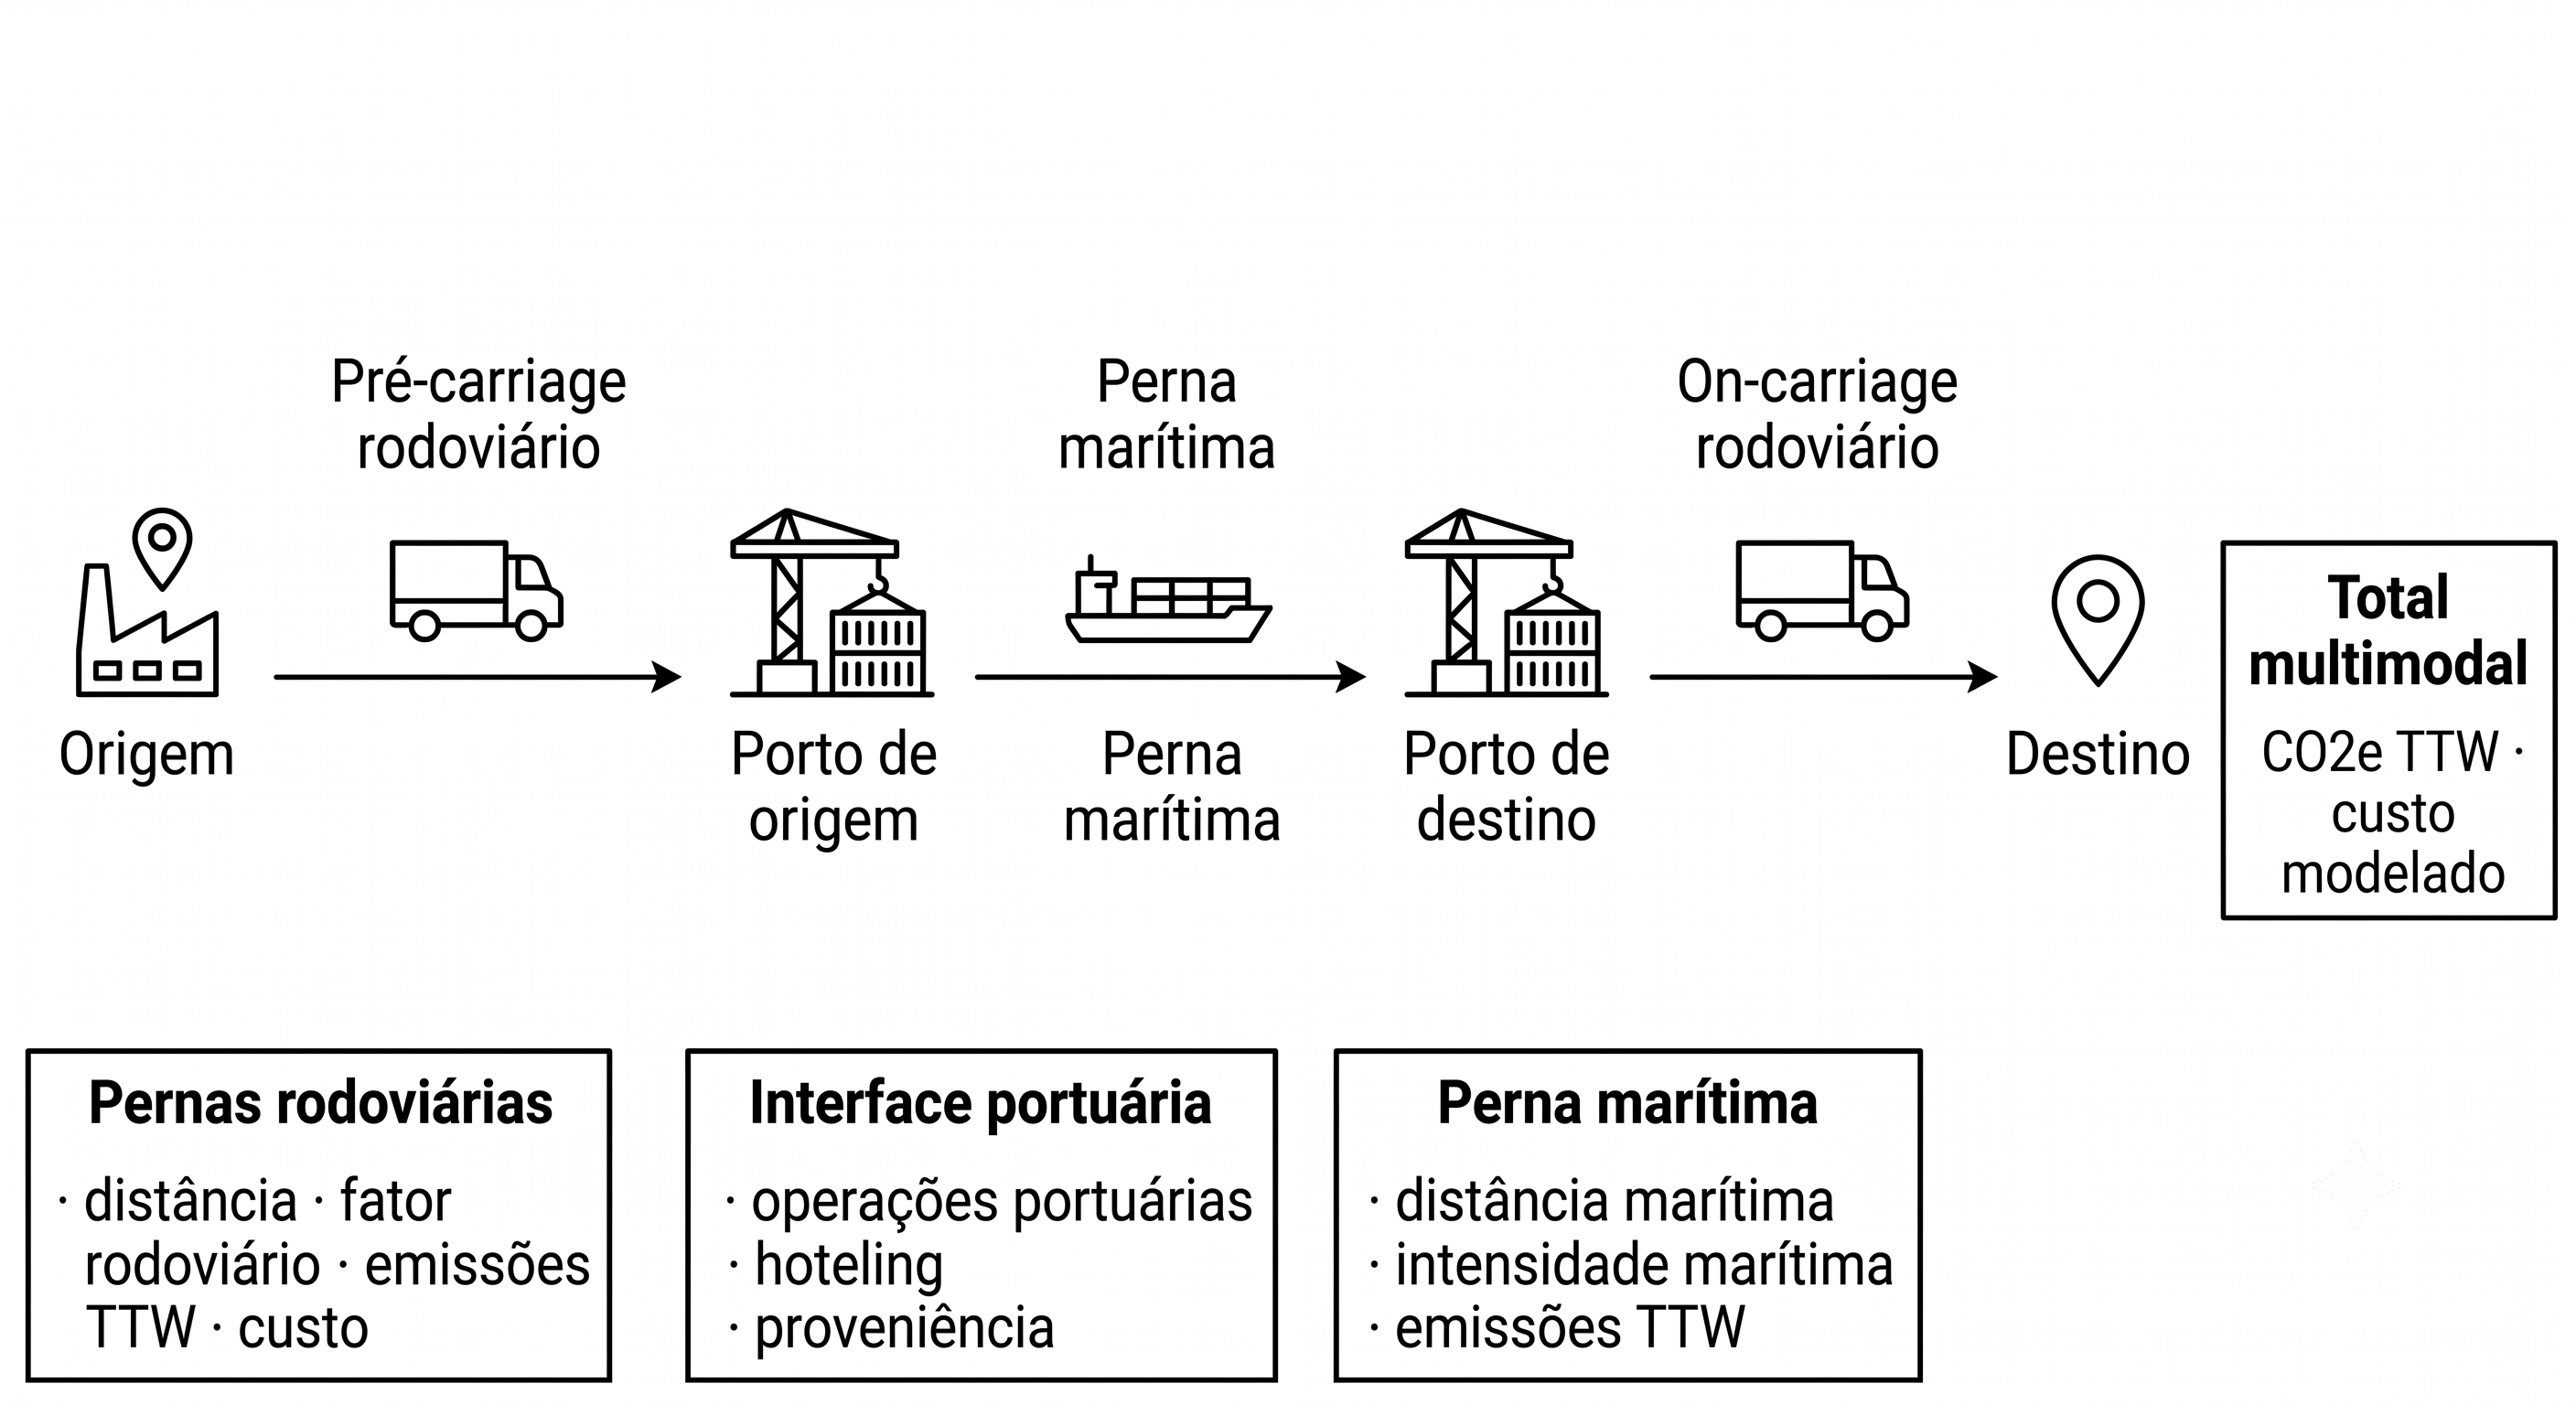
\includegraphics[width=0.95\textwidth]{images/figura_4_1.png}
\caption{Decomposição metodológica da alternativa multimodal em pernas rodoviárias, interface portuária, perna marítima e agregação final.}
\label{fig:cadeia-multimodal}
\end{figure}

A Figura~\ref{fig:cadeia-multimodal} evidencia a regra de agregação por componentes. O total multimodal não é a perna marítima isolada: é a soma dos acessos terrestres, da navegação e dos componentes portuários incluídos, cada um com distância, fator, custo e proveniência próprios.

\begin{equation}
R_{\mathrm{multi}} = R_{\mathrm{pre}} + R_{\mathrm{mar}} + R_{\mathrm{port}} + R_{\mathrm{on}}
\label{eq:multimodal-aggregation}
\end{equation}

Na Equação~\ref{eq:multimodal-aggregation}, \(R_{\mathrm{multi}}\) representa o resultado agregado da alternativa multimodal para uma dimensão de saída, como custo modelado ou emissões operacionais; \(R_{\mathrm{pre}}\) é o acesso rodoviário inicial; \(R_{\mathrm{mar}}\) é a perna marítima; \(R_{\mathrm{port}}\) representa operações portuárias e \emph{hoteling} incluídos; e \(R_{\mathrm{on}}\) é o acesso rodoviário final. A fórmula apenas explicita a composição do total e preserva a separação entre pernas.

\section{Reconstrução das viagens e formulação da intensidade marítima}
\label{sec:intensidade-maritima}

A estimativa marítima combina os registros de Carga e Atracação da ANTAQ com os indicadores de eficiência do EU MRV. A tabela de Carga registra movimentações associadas às escalas, incluindo massa, quantidade e portos relacionados à origem e ao destino da carga. A tabela de Atracação fornece a sequência temporal das escalas e o número IMO do navio. Depois da normalização dos nomes e códigos portuários, as escalas de cada viagem são ordenadas e chamadas consecutivas pertencentes ao mesmo complexo portuário são consolidadas sem descartar as movimentações de carga correspondentes.

Para um par de portos \((o,d)\), uma observação é elegível quando \(o\) aparece antes de \(d\) na sequência da mesma viagem. O procedimento examina todas as viagens elegíveis e todos os corredores observados entre o par, incluindo ligações diretas e percursos com uma ou mais escalas intermediárias. Não se impõe uma sequência fixa de portos. Se o mesmo par aparecer mais de uma vez dentro de uma viagem, mantém-se uma única observação dessa viagem para evitar dupla contagem; a escolha é determinística, priorizando a ocorrência direta e, na ausência dela, a de menor distância completa.

Seja \(\Delta m_{v,j}\) a movimentação líquida de massa na escala \(j\) da viagem \(v\), positiva para acréscimo líquido de carga a bordo e negativa para redução líquida. Como a janela observada pode começar com carga já embarcada, calcula-se uma carga inicial mínima que impeça valores negativos ao longo da sequência:

\begin{equation}
m_{v,0}=\max\left(0,-\min_k\sum_{j=1}^{k}\Delta m_{v,j}\right).
\label{eq:carga-inicial-maritima}
\end{equation}

A carga a bordo no subtrecho iniciado após a escala \(j\) é, então,

\begin{equation}
m_{v,j}=\max\left(0,m_{v,0}+\sum_{r=1}^{j}\Delta m_{v,r}\right).
\label{eq:carga-bordo-subtrecho}
\end{equation}

Essa reconstrução por saldo acumulado faz com que cada subtrecho use a massa efetivamente representada a bordo naquele ponto da viagem, em vez de atribuir a mesma carga a toda a sequência. Para a observação de \(o\) a \(d\), formada pelos subtrechos \(S_{v,o,d}\), o trabalho de transporte e o consumo de combustível alocado são dados por

\begin{equation}
\begin{aligned}
W_{v,o,d} &= \sum_{s\in S_{v,o,d}} m_{v,s}\,d_s, \\
F_{v,o,d} &= I_v\,W_{v,o,d}.
\end{aligned}
\label{eq:trabalho-consumo-viagem}
\end{equation}

em que \(d_s\) é a distância do subtrecho em milhas náuticas, \(W_{v,o,d}\) é expresso em \(\mathrm{t\,nm}\), \(I_v\) é a intensidade atribuída ao navio em \(\mathrm{g/(t\,nm)}\), e \(F_{v,o,d}\) é obtido em gramas. Assim, uma viagem com escalas intermediárias contribui pela soma de todos os subtrechos entre a origem e o destino, mantendo a carga a bordo e a distância próprias de cada um.

A intensidade \(I_v\) segue uma hierarquia de proveniência. A primeira opção é o valor positivo mais recente do EU MRV associado exatamente ao IMO observado na ANTAQ. Na ausência de correspondência, usa-se a estatística robusta da classe de embarcação, quando a classe está disponível; em seguida, usa-se a estatística do tipo de navio. Para o escopo conteinerizado, \emph{Container ship} é o tipo-padrão documentado quando o registro não oferece classificação mais específica. Se nenhuma etapa produz valor positivo, a intensidade da viagem permanece indisponível e essa ocorrência é contabilizada como não resolvida.

Os valores exatos por IMO são preservados sem corte, pois representam o indicador individual do navio. A regra de outliers aplica-se somente às estatísticas de fallback. Para o tipo de navio, os valores positivos mais recentes por IMO são ordenados e removem-se simetricamente \(\lfloor 0{,}01n\rfloor\) observações de cada cauda antes da média. Quando a amostra é pequena demais para retirar ao menos uma observação de cada lado, usa-se a mediana. Para a classe, utiliza-se a média aparada simétrica de 1\% em cada cauda registrada no artefato, operacionalizada pela exclusão dos valores abaixo do percentil 1 e acima do percentil 99; a mediana é usada quando essa estatística não está disponível. A fonte final registra o nível usado --- IMO, classe ou tipo --- e, nos fallbacks agregados, a estatística, o tamanho da amostra e a regra de outlier aplicável.

Uma única intensidade representativa é calculada para cada par ordenado de portos a partir de todas as observações de viagem com intensidade resolvida, sem restringir a amostra ao corredor escolhido para a geometria. Cada intensidade \(I_v\) recebe como peso o trabalho de transporte completo \(W_{v,o,d}\) da respectiva observação. A intensidade do par é a mediana ponderada, definida pela primeira intensidade na ordem crescente cuja soma acumulada dos pesos alcança 50\% do trabalho de transporte total:

\begin{equation}
I_{o,d}=\min\left\{x:\sum_{v:I_v\leq x}W_{v,o,d}\geq
\frac{1}{2}\sum_v W_{v,o,d}\right\}.
\label{eq:mediana-ponderada-intensidade}
\end{equation}

Observações com trabalho de transporte nulo não influenciam a Equação~\ref{eq:mediana-ponderada-intensidade} quando existe ao menos um peso positivo. Se todas as observações resolvidas do par tiverem trabalho nulo, adota-se a mediana não ponderada dessas intensidades e a fonte identifica explicitamente essa condição. A ausência de qualquer intensidade resolvida permanece indisponível, sem conversão para zero.

A estatística de intensidade e a escolha do caminho cumprem funções distintas. Todas as observações elegíveis com intensidade resolvida e trabalho positivo, distribuídas entre os diferentes corredores do par, alimentam a intensidade \(I_{o,d}\); o caminho usado no cenário é selecionado apenas para definir a sequência de portos e as distâncias navegadas. O critério geométrico prioriza um corredor direto observado e, entre alternativas da mesma categoria, a menor distância; sem corredor direto utilizável, escolhe-se o corredor multitrecho de menor distância. A intensidade observada do corredor selecionado é preservada como diagnóstico, mas não substitui a intensidade representativa do par.

Para uma remessa de massa \(m_{\mathrm{cen}}\), a navegação no cenário aplica \(I_{o,d}\) a cada distância do caminho selecionado:

\begin{equation}
F_{\mathrm{mar,cen}}=\frac{I_{o,d}\,m_{\mathrm{cen}}}{1000}
\sum_{s\in S_{\mathrm{sel}}}d_s,
\label{eq:combustivel-maritimo-cenario}
\end{equation}

em que o divisor converte gramas em quilogramas. Essa formulação mantém todos os corredores na estimação estatística, ao mesmo tempo que fornece uma geometria única e auditável para distância, combustível, custo modelado e emissões operacionais do cenário.

\section{Seleção de portos e definição de cenários}
\label{sec:selecao-portos}

A seleção de portos transforma a unidade funcional em uma cadeia multimodal concreta. Para uma mesma origem, destino e carga, diferentes portos podem alterar o comprimento do \emph{pre-carriage}, a distância marítima, o \emph{on-carriage}, os componentes portuários e a força da evidência disponível.

O método distingue três situações. Na seleção automática, portos elegíveis são escolhidos por uma lógica determinística e auditável dentro do conjunto configurado. Na seleção forçada ou manual, o cenário impõe porto de origem ou destino para representar uma hipótese específica, um benchmark ou uma análise controlada. Em cenários de sensibilidade, portos alternativos podem ser testados para avaliar como uma substituição declarada altera a comparação.

Essas situações não são intercambiáveis. Um porto selecionado para o caso-base, um porto forçado por hipótese e um porto alternativo de sensibilidade devem permanecer identificados como tal. Não há substituição silenciosa de um porto por outro: Pecém não valida Porto de Fortaleza, Suape não valida Porto do Recife, e um cenário alternativo não redefine automaticamente o cenário selecionado originalmente \cite{competitiveness2024,modalshiftreview2020}.

Essa seleção também não equivale a uma otimização comercial de rede. O método não resolve grade de navegação, frequência de escalas, disponibilidade de armador, slot, tempo de trânsito, confiabilidade, estoque em trânsito ou decisão de contratação. Esses elementos pertencem a uma fronteira de modelagem mais ampla.

\section{Proveniência das distâncias e hierarquia de confiança}
\label{sec:proveniencia-distancias}

A distância é um dos principais controles metodológicos do capítulo. Na alternativa rodoviária direta, ela define a perna origem-destino. Na alternativa multimodal, ela aparece separadamente no \emph{pre-carriage}, nos subtrechos do corredor marítimo selecionado e no \emph{on-carriage}. Por isso, dois cenários com totais calculados semelhantes podem ter força interpretativa diferente se a proveniência das distâncias for diferente. A origem da distância é registrada por subtrecho: usa-se primeiro um valor positivo da matriz marítima e, quando ele não existe para portos canônicos distintos, uma aproximação por coordenadas identificada como \texttt{haversine\_fallback}.

\begin{table}[htbp]
\centering
\small
\caption{Hierarquia de proveniência de distâncias.}
\label{tab:proveniencia-distancias}
\begin{tabularx}{\textwidth}{L{0.24\textwidth}Y Y}
\toprule
Proveniência & Uso metodológico & Limite de interpretação \\
\midrule
Roteamento rodoviário/cache & Distância modelada para pernas terrestres. & Não é trajetória GPS medida nem rota comercial efetivamente usada.\\
\texttt{seamatrix} & Distância marítima matricial para par de portos aplicável. & Não comprova escala, frequência, serviço ou contrato.\\
\texttt{external\_reference} & Referência documentada para o par de portos do cenário. & Só vale para o par e a unidade documentados.\\
\texttt{manual\_override} & Substituição explícita e rastreável para um cenário. & Exige motivação documentada; não deve ser generalizada.\\
\texttt{haversine\_fallback} & Estimativa geométrica quando falta distância marítima documentada. & Triagem ou lacuna de evidência; não valida rota marítima.\\
Referência ausente & Indica que a distância necessária não está suficientemente documentada. & Pode bloquear conclusão ou limitar o caso a sensibilidade.\\
\bottomrule
\end{tabularx}
\end{table}

Na Tabela~\ref{tab:proveniencia-distancias}, \texttt{seamatrix} e \texttt{external\_reference} oferecem evidência mais forte para a distância marítima porque representam uma matriz ou referência documentada para o par de portos. \texttt{manual\_override} pode ser adequado quando a substituição é explícita e justificada, mas sua validade fica restrita ao cenário. \texttt{haversine\_fallback} é útil para triagem quando falta referência marítima, porém tem menor força para conclusões numéricas. Essa hierarquia afeta a classificação da evidência; não altera, por si só, o fator de emissão ou a fronteira econômica.

\section{Cadeias conceituais de cálculo de emissões e custos}
\label{sec:cadeias-calculo}

Os cálculos são organizados como cadeias conceituais de transformação. Para cada perna rodoviária, a distância, a configuração de veículo e a carga definem o consumo estimado; o consumo e o fator implementado definem emissões operacionais \ttw{} de \cooe{}; o consumo e os insumos econômicos definem custo operacional modelado. Para a perna marítima, a intensidade representativa do par, a massa da remessa e as distâncias dos subtrechos selecionados definem o consumo de navegação conforme a Equação~\ref{eq:combustivel-maritimo-cenario}; esse consumo alimenta as emissões marítimas e o custo marítimo modelado.

Na alternativa rodoviária direta, há uma única cadeia de perna. Na alternativa multimodal, as cadeias do \emph{pre-carriage}, da perna marítima, dos componentes portuários e do \emph{on-carriage} são calculadas separadamente e depois agregadas. Essa decomposição preserva a distinção entre distância, consumo, custo e emissões, além de permitir que a proveniência de cada componente acompanhe o total.

Custos e emissões são dimensões metodológicas diferentes. O método pode mostrar que uma alternativa apresenta menor emissão, menor custo modelado, ambos, ou divergência entre essas dimensões. A interpretação exige que os componentes incluídos no total estejam declarados e que a comparação permaneça vinculada à mesma unidade funcional.

\section{Operações portuárias, hoteling e proveniência dos dados}
\label{sec:portops-metodologia}

Operações portuárias e \emph{hoteling} são tratados como componentes da cadeia multimodal quando incluídos na fronteira do cenário. Eles podem acrescentar consumo, emissões e custo modelado associados à permanência em porto, ao uso de sistemas auxiliares e às atividades de terminal. Sua inclusão depende de proveniência suficiente para indicar que tipo de componente foi representado, em qual porto ou condição, com qual unidade e sob qual fronteira \cite{berth2009,shipops2022,decarb2024}.

Quando há dado específico para o porto selecionado, o componente pode ser registrado como \texttt{observed}. Quando o dado específico não existe, a ausência não é interpretada como zero. O método usa uma hierarquia explícita: \texttt{estimated\_port\_average}, quando há média ponderada defensável de portos observados; \texttt{literature\_default}, quando há apenas um padrão documentado do modelo; ou \texttt{unavailable}, quando nenhum valor observado ou documentado pode ser atribuído.

A regra de consistência é evitar dupla contagem. Quando o cenário utiliza a intensidade MRV por trabalho de transporte, o indicador anual é tratado, para essa fronteira, como abrangente do consumo reportado do navio e o \emph{hoteling} não é acrescentado separadamente. As operações de terminal permanecem componentes explícitos quando têm proveniência representável. Nos modos em que navegação, permanência em porto e operação de terminal são modeladas separadamente, essa decomposição deve aparecer nos metadados e na interpretação do resultado.

\section{Qualidade de rota, classificação de evidências e limites de uso}
\label{sec:qualidade-evidencias}

A classificação de evidências é o mecanismo de controle de qualidade metodológica do TF. Antes de transformar um resultado calculado em argumento, o método verifica se a cadeia é comparável, se a distância tem proveniência suficiente, se os portos correspondem ao cenário declarado, se a fronteira ambiental e econômica foi preservada e se existem avisos como \emph{same-port}, \texttt{haversine\_fallback}, referência ausente ou porto alternativo.

\begin{table}[htbp]
\centering
\small
\caption{Classificações metodológicas usadas para controlar inferências.}
\label{tab:classificacoes-metodologia}
\begin{tabularx}{\textwidth}{L{0.28\textwidth}Y Y}
\toprule
Condição ou classificação & Significado metodológico & Uso seguro \\
\midrule
\codecell{observed\_input} & Registro de atividade com fonte, período e transformação identificados. & Reconstrução e auditoria dentro do recorte documentado.\\
\codecell{reference\_needed} & Falta evidência suficiente para distância ou premissa necessária. & Lacuna e prioridade de validação futura.\\
\codecell{excluded} & Caso inválido ou fora da fronteira adotada. & Justificativa de exclusão, sem uso numérico conclusivo.\\
\codecell{sensitivity\_only} / \codecell{sensitive} & Cenário ou resultado sob hipótese condicional. & Discussão condicionada, sem substituir caso-base.\\
\codecell{headline\_candidate} & Resultado com rota, fonte, unidade, fronteira e comparabilidade suficientes. & Uso como síntese principal somente dentro do escopo documentado.\\
\bottomrule
\end{tabularx}
\end{table}

A Tabela~\ref{tab:classificacoes-metodologia} antecipa a função da validação no Capítulo~\ref{ch:validacao}. Benchmarks externos, incluindo materiais associados ao Prof. Dr. Gustavo Costa, entram como comparação e diagnóstico de fronteiras. Eles podem apoiar uma leitura direcional ou revelar diferenças de premissa, mas não redefinem o caso-base, não calibram magnitudes sem alinhamento metodológico completo e não transformam custo modelado em frete comercial.

\chapter{Ferramenta computacional}
\label{ch:implementacao}

\section{Visão geral da ferramenta e arquitetura do protótipo}
\label{sec:visao-geral-ferramenta}

O \CabotageLens{} transforma a metodologia do Capítulo~\ref{ch:metodologia} em uma execução computacional. O usuário informa um cenário. O programa constrói a alternativa rodoviária direta e a alternativa rodoviária--cabotagem--rodoviária. A saída apresenta o resultado de cada trecho, os totais, as fontes e os avisos.

O objetivo não é contratar transporte. O objetivo é permitir que outra pessoa compreenda e confira o cálculo. Um cálculo que permite essa conferência é chamado de auditável. Para isso, o sistema preserva a origem e o destino, a carga, os portos, as coordenadas, as rotas, o estado do cache, a fonte da distância marítima, a cobertura ANTAQ/MRV, os preços, o modo de alocação, os componentes incluídos e os avisos de qualidade.

Em termos de arquitetura, o protótipo possui três camadas fáceis de distinguir:

\begin{itemize}
  \item \textbf{Entrada:} interface, parâmetros do cenário e dados processados.
  \item \textbf{Processamento:} geocodificação, roteamento, seleção de portos, construção das pernas e cálculos.
  \item \textbf{Saída:} comparação, detalhamento, fontes e tratamentos dos dados, avisos, persistência e exportação.
\end{itemize}

\begin{figure}[htbp]
\centering
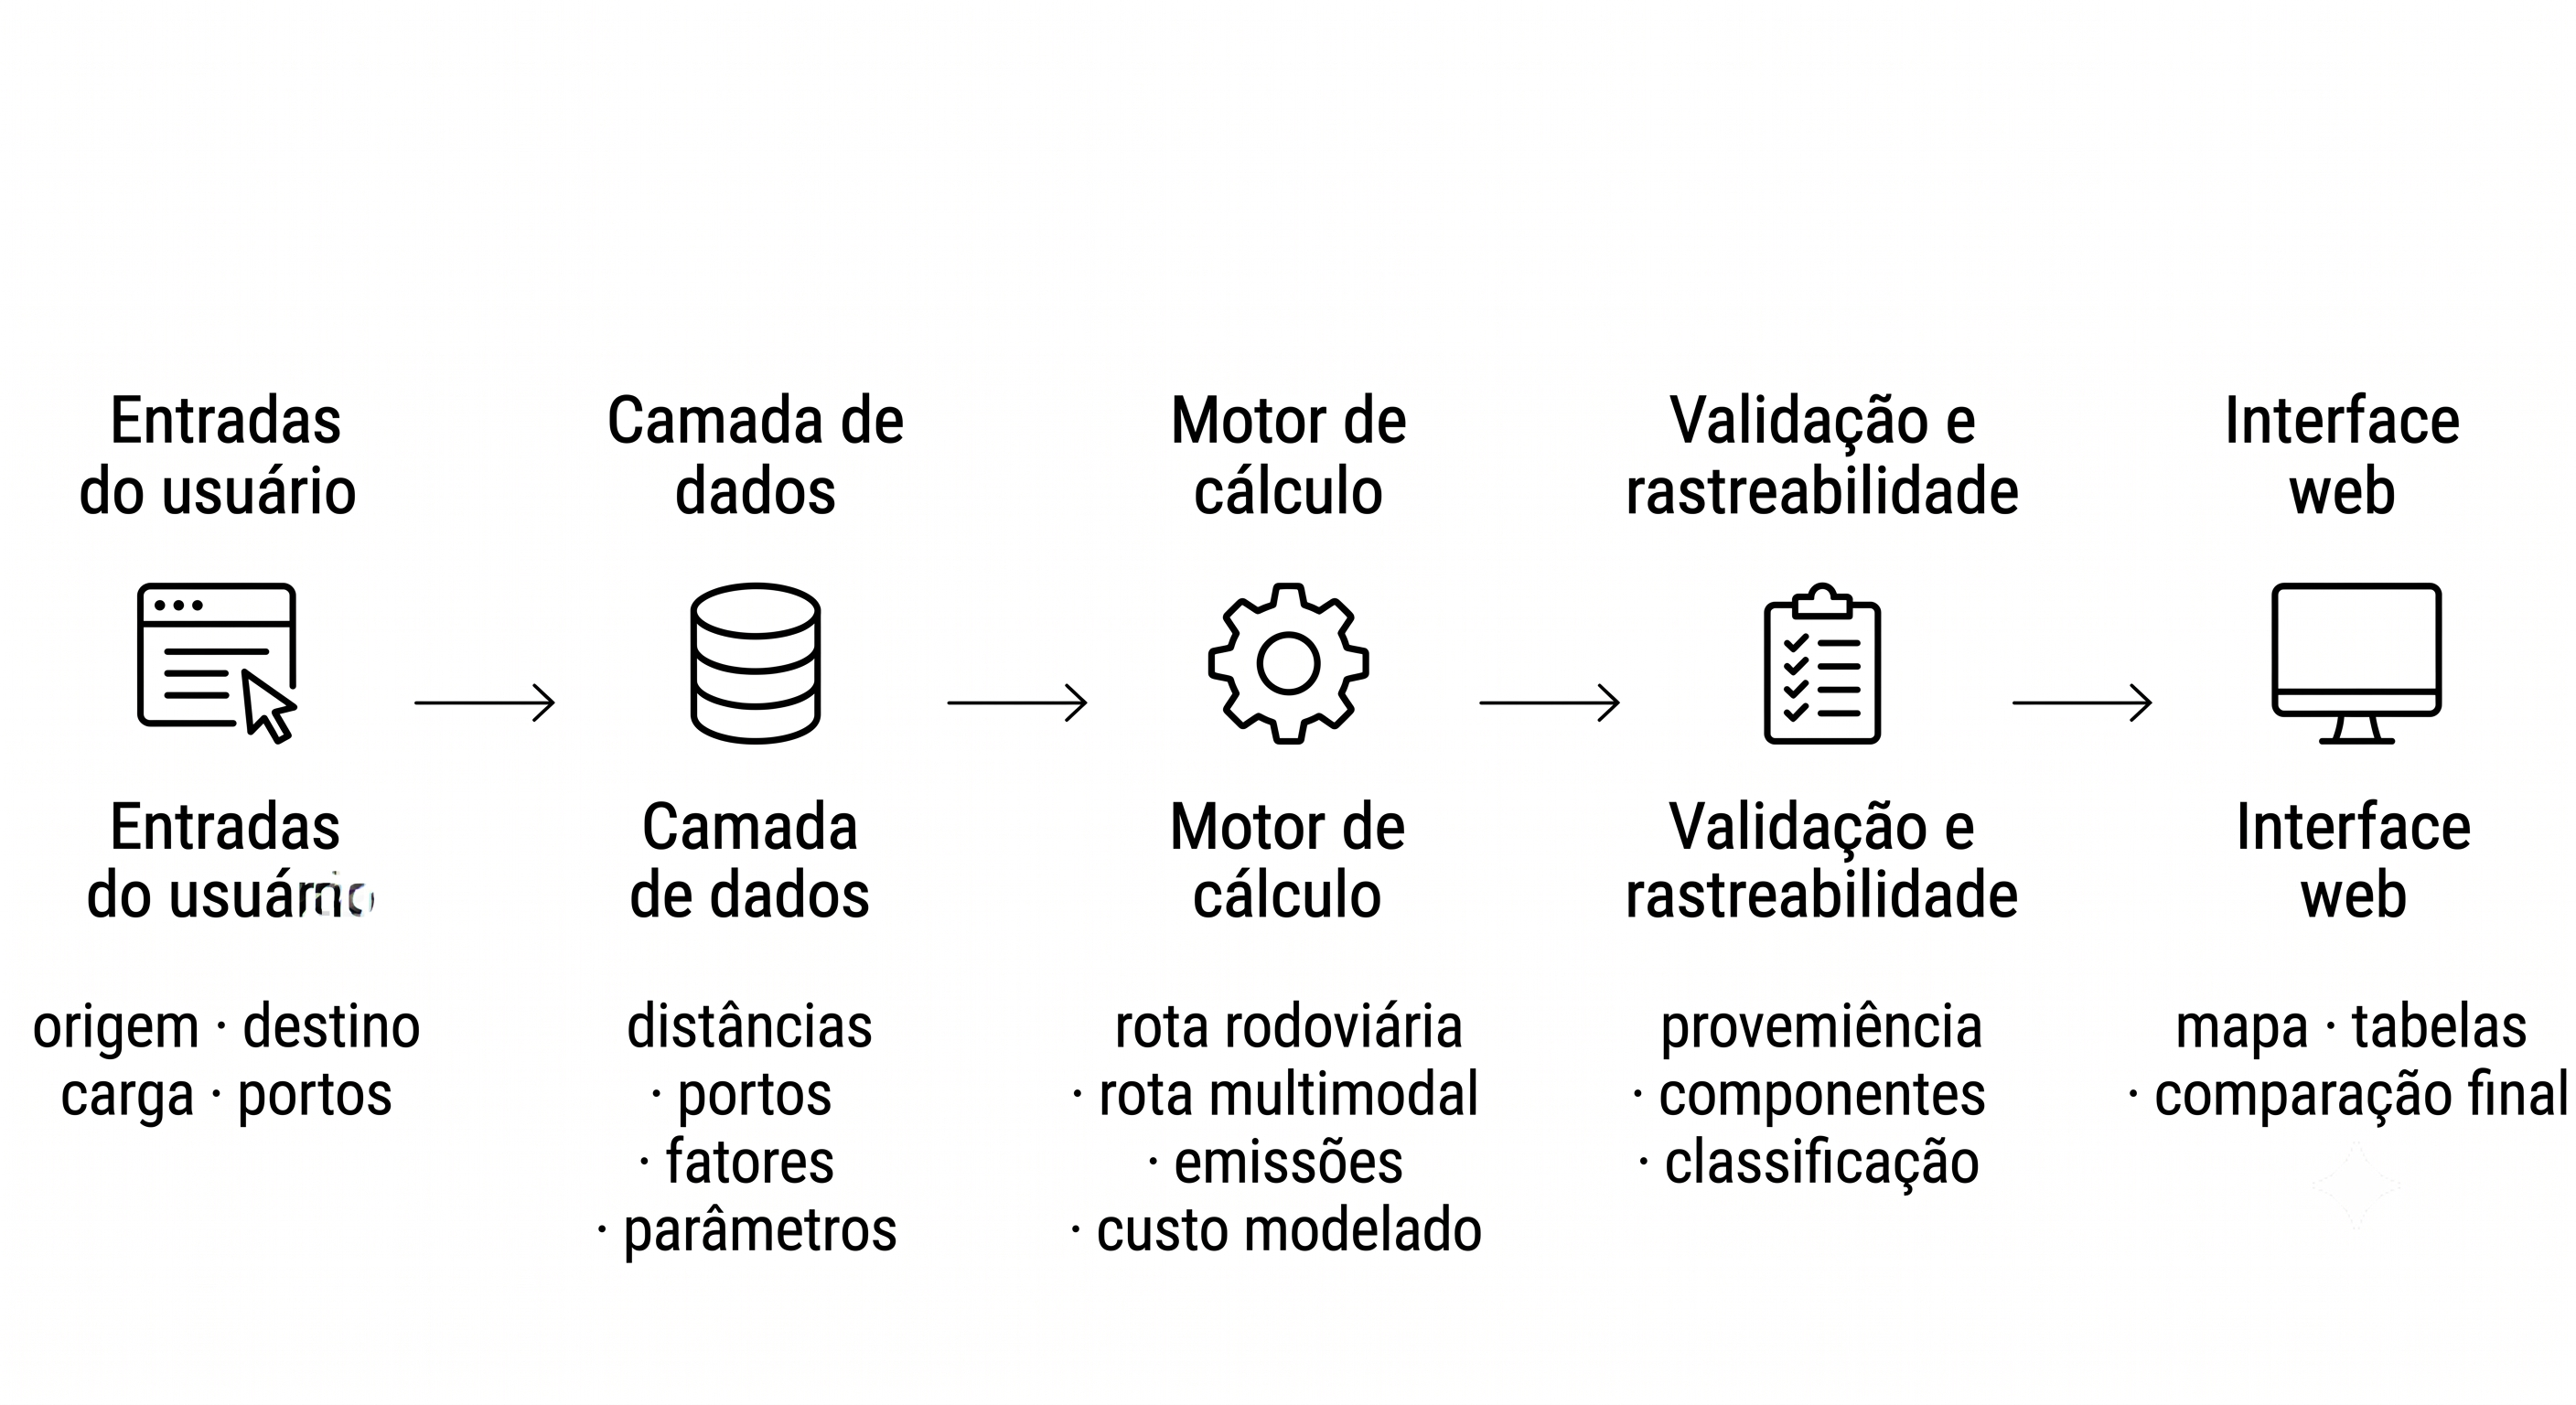
\includegraphics[width=0.95\textwidth]{images/figura_5_1.png}
\caption{Arquitetura computacional simplificada da ferramenta, desde as entradas do usuário e a camada de dados até o motor de cálculo, a rastreabilidade e a interface web.}
\label{fig:arquitetura-computacional}
\end{figure}

\section{Dois fluxos computacionais: execução do cenário e preparação histórica}
\label{sec:fluxos-computacionais}

O sistema possui dois fluxos. Eles se complementam, mas não são executados ao mesmo tempo.

O primeiro é a \textbf{execução de cenário}. Ele começa quando o usuário informa a origem da carga, o destino final da carga e a massa da remessa. A sequência é: entrada do cenário \(\rightarrow\) localização dos pontos no mapa \(\rightarrow\) cálculo ou reaproveitamento das rotas terrestres \(\rightarrow\) seleção do porto de embarque e do porto de desembarque \(\rightarrow\) consulta da matriz marítima já preparada \(\rightarrow\) obtenção dos dados necessários \(\rightarrow\) cálculo de cada parte da viagem \(\rightarrow\) resultados e avisos.

O segundo é a \textbf{preparação dos dados históricos}, realizada antes das simulações do usuário. O processo baixa e integra as tabelas da ANTAQ. Depois, separa os registros por viagem e coloca as escalas da mais antiga para a mais recente. O sistema calcula a carga histórica que permaneceu no navio em cada trecho. Em seguida, procura no EU MRV o consumo correspondente ao IMO. Quando não encontra o IMO, aplica uma regra substituta baseada na classe ou no tipo do navio. Por fim, reúne todas as sequências de portos observadas entre cada porto de embarque e cada porto de desembarque. O resultado é a matriz marítima usada pela aplicação. Quando configurados, Supabase/Postgres ou Supabase Storage podem sincronizar esses arquivos processados.

\begin{table}[htbp]
\centering
\small
\caption{Fluxos computacionais principais do \CabotageLens{}.}
\label{tab:fluxos-computacionais}
\begin{tabularx}{\textwidth}{L{0.22\textwidth}Y Y Y}
\toprule
Fluxo & O que entra & O que transforma & O que entrega ao TF \\
\midrule
Execução de cenário & Origem da carga, destino final da carga, massa da remessa do usuário, portos selecionados e parâmetros. & Consulta rotas e a matriz já preparada; aplica a massa do usuário às distâncias do cenário; calcula combustível, custos e emissões. & Comparação rastreável entre rodovia direta e cadeia multimodal, com avisos e metadados.\\
Preparação histórica offline & Tabelas ANTAQ, dados EU MRV e ativos locais de matriz, preços e parâmetros. & Ordena as escalas da mesma viagem, calcula a carga histórica em cada trecho, busca o consumo por IMO e reúne as diferentes sequências entre portos de embarque e desembarque. & Indicadores marítimos documentados que serão consultados pelos cenários.\\
\bottomrule
\end{tabularx}
\end{table}

A Tabela~\ref{tab:fluxos-computacionais} mostra a separação de responsabilidades. A preparação histórica produz a matriz. A execução consulta essa matriz pronta. A carga histórica a bordo pondera a intensidade durante a preparação. A massa da remessa informada pelo usuário entra somente na execução do cenário. Assim, o sistema não aplica duas vezes a carga histórica.

\section{Entradas do cenário, geocodificação e roteamento terrestre}
\label{sec:entradas-geocodificacao-roteamento}

\textbf{Entradas do usuário.} Um cenário pode conter a origem da carga, o destino final da carga, a massa, o TEU ou a relação t/TEU, a escolha do porto de embarque e do porto de desembarque, a classe de embarcação, o caminhão, o modo de alocação, os preços de combustíveis, as operações portuárias, o \emph{hoteling} e as opções de exportação. A origem e o destino são locais da remessa porta a porta. Os portos delimitam somente a perna marítima.

\textbf{Geocodificação.} O programa transforma nomes de lugares em latitude, longitude, rótulo e UF quando identificável. Primeiro, procura uma coordenada persistida. Se necessário, consulta OpenRouteService. LocationIQ pode atuar como provedor substituto, ou \emph{fallback}, quando configurado. As respostas são normalizadas para que as etapas seguintes não dependam do formato particular de cada provedor.

\textbf{Roteamento terrestre.} Para cada perna rodoviária, o sistema consulta primeiro as rotas já armazenadas no Supabase/Postgres. Somente quando não encontra um registro chama um serviço externo. Essa ordem recebe internamente o nome de \emph{cache-first}. Se o provedor calcular uma rota, o sistema tenta armazenar a resposta.

\textbf{Saída da etapa.} Cada perna terrestre conserva coordenadas, distância, perfil de rota, provedor, fonte e indicação de acerto ou falha de cache. Essas distâncias são rotas modeladas. Elas não são trajetórias GPS observadas nem confirmação de uma rota contratual.

\section{Construção das alternativas, seleção de portos e perna marítima}
\label{sec:construcao-alternativas}

Depois de resolver os lugares, o sistema constrói duas alternativas. A primeira liga a origem da carga ao destino final da carga por rodovia. A segunda divide o percurso em três partes principais: acesso rodoviário da origem da carga ao porto de embarque; navegação até o porto de desembarque; e acesso rodoviário até o destino final da carga. Essa divisão permite medir quanto cada componente contribui para o total.

O porto de embarque e o porto de desembarque podem ser selecionados automaticamente, forçados pelo usuário ou substituídos em uma análise de sensibilidade. A saída identifica qual situação foi usada. A seleção de um porto não confirma frequência, slot, armador ou aceitação terminal.

Para a navegação, o sistema consulta a matriz marítima. A direção importa. Santos--Manaus significa embarcar em Santos e desembarcar em Manaus. Manaus--Santos significa fazer o sentido contrário. A matriz guarda essas duas ligações separadamente. Para cada combinação de porto de embarque e porto de desembarque, ela fornece:

\begin{itemize}
  \item a intensidade representativa calculada com todos os recortes históricos aceitos entre esses portos;
  \item a sequência de portos escolhida para fornecer as distâncias do cenário;
  \item as demais sequências de portos observadas entre a mesma partida e a mesma chegada;
  \item as quantidades de valores obtidos por IMO, classe ou tipo;
  \item a fonte de cada distância marítima.
\end{itemize}

O programa usa uma intensidade para toda a ligação entre o porto de embarque e o porto de desembarque. A intensidade informa quantos gramas de combustível representam o transporte de uma tonelada por uma milha náutica. Para calcular a distância, o programa escolhe uma sequência completa de portos observada. Essa é a rota marítima usada na execução do cenário.

A intensidade calculada somente com os recortes cujo corredor coincide com a sequência escolhida permanece disponível para diagnóstico. Ela não substitui a intensidade representativa calculada com todos os recortes aceitos entre o porto de embarque e o porto de desembarque. Se faltar uma distância positiva entre dois portos diferentes, o sistema pode usar uma aproximação em linha reta baseada nas coordenadas. O identificador interno dessa aproximação é \codecell{haversine\_fallback}. A interface avisa quando isso ocorre. Avisos de mesmo porto nas duas extremidades (\emph{same-port}), distância ausente e regra substituta limitam a interpretação.

\section{Pipeline marítimo offline}
\label{sec:pipeline-maritimo-offline}

O processamento feito antes do uso da aplicação produz a matriz marítima. Ele prepara indicadores históricos; não calcula ainda a remessa do usuário. Internamente, esse processamento recebe o nome de \emph{pipeline offline}. As etapas seguem esta ordem:

\begin{enumerate}
  \item reunir as chamadas do mesmo navio pelo IMO, ordená-las por data e iniciar uma nova viagem quando o navio retorna ao porto inicial ou quando o intervalo entre paradas supera 240 horas;
  \item dentro da mesma viagem, manter as atracações da mais antiga para a mais recente e padronizar os nomes dos portos;
  \item consolidar chamadas consecutivas no mesmo porto sem perder embarques ou desembarques;
  \item reconstruir a carga histórica a bordo com as Equações~\ref{eq:carga-inicial-maritima} e \ref{eq:carga-bordo-subtrecho};
  \item verificar se a viagem realmente percorreu a direção pedida. No cálculo Santos--Manaus, por exemplo, a parte aproveitada da viagem precisa começar na escala de Santos e terminar na escala de Manaus. O sistema usa o recorte Santos--Suape--Pecém--Manaus da viagem real \codecell{voyage\_9612791\_00011}; uma passagem em que Manaus apareça antes de Santos não entra;
  \item conservar todos os trechos consecutivos entre os dois portos, tanto em passagens diretas quanto em passagens com portos intermediários;
  \item manter no máximo um recorte histórico viagem--OD por viagem e por ligação; diante de repetição, preferir a passagem direta e depois a sequência completa de menor distância, o menor número de trechos e a ordem das escalas;
  \item procurar a intensidade pelo IMO, pela classe e pelo tipo, nessa ordem; registrar quando nenhum deles fornecer um valor positivo;
  \item reunir os recortes que receberam uma intensidade, aplicar os pesos de trabalho de transporte e escolher separadamente uma sequência de portos para fornecer as distâncias do cenário.
\end{enumerate}

Para cada recorte aceito, o sistema guarda somente o deslocamento entre os dois portos escolhidos. Esse objeto recebe o nome de \emph{recorte histórico viagem--OD}, em que OD significa origem--destino. Ele contém todos os subtrechos consecutivos entre o porto inicial e o porto final. Cada subtrecho armazena os portos inicial e final, sua posição na sequência, a carga em toneladas e TEU, a distância, a fonte da distância, o trabalho de transporte, a intensidade, o combustível e a indicação de que nenhum subtrecho está ausente. A mesma estrutura representa recortes diretos e recortes com escalas.

A carga histórica muda depois de cada escala. O sistema soma o que foi embarcado e subtrai o que foi desembarcado. Na viagem \codecell{voyage\_9612791\_00011}, a carga inicial reconstruída foi \(2.976{,}894\)~t. O saldo de \(+9.881{,}860\)~t em Santos fez o navio seguir para Suape com \(12.858{,}754\)~t. Depois do saldo de \(+3.859{,}579\)~t em Suape, ele seguiu para Pecém com \(16.718{,}333\)~t. O saldo de \(-4.392{,}433\)~t em Pecém reduziu a carga do trecho seguinte, até Manaus, para \(12.325{,}900\)~t. Essa reconstrução define o peso histórico do indicador. Ela não substitui a massa da remessa informada pelo usuário durante a execução.

O sistema procura primeiro a intensidade do próprio navio pelo IMO. A intensidade mede gramas de combustível por tonelada-milha náutica. Para o IMO, o sistema utiliza o valor positivo mais recente do MRV. Esse valor individual não é alterado pela regra de retirada de valores extremos.

Se o IMO não tiver correspondência, o sistema segue regras substitutas definidas antes do cálculo. Essas regras recebem o nome de fallback.

\textbf{Fallback por classe.} Quando conhece a classe do navio, o sistema usa primeiro a média registrada no arquivo de eficiência depois de excluir os valores abaixo do percentil 1 e acima do percentil 99. Se essa média não estiver disponível, usa a mediana da classe.

\textbf{Fallback por tipo.} Se a classe não fornecer um valor positivo, o sistema reúne os valores positivos mais recentes dos navios do mesmo tipo. Ordena os valores, remove \(\lfloor0{,}01n\rfloor\) de cada extremidade e calcula a média do restante. Se a amostra for pequena demais para remover pelo menos um valor de cada lado, usa a mediana do tipo. Para carga conteinerizada, pode usar o tipo-padrão documentado \emph{Container ship}.

Se IMO, classe e tipo não fornecerem uma intensidade positiva, o sistema registra que o valor não está disponível. Ele não troca a ausência por zero.

O sistema reúne todos os recortes aprovados para a direção pedida. No cálculo Santos--Manaus, por exemplo, entram tanto o recorte direto da viagem \codecell{voyage\_9612789\_00004} quanto o recorte Santos--Suape--Pecém--Manaus da viagem \codecell{voyage\_9612791\_00011}. Uma passagem Manaus--Santos não entra, pois representa a direção contrária. Em cada recorte aprovado, o sistema multiplica a carga a bordo pela distância de cada trecho e soma os produtos. Essa soma é o trabalho de transporte.

O trabalho de transporte funciona como peso na Equação~\ref{eq:mediana-ponderada-intensidade}. O sistema ordena as intensidades e escolhe a primeira que alcança pelo menos metade do peso total acumulado. Esse resultado é a mediana ponderada. Pesos nulos são ignorados quando existe trabalho positivo. Se todos forem nulos, o sistema usa a mediana sem pesos e registra essa condição.

Depois, o sistema escolhe uma única sequência de portos para fornecer as distâncias do cenário. A regra procura primeiro uma ligação direta. Se ela não existir, escolhe a sequência completa de menor distância. O identificador interno dessa regra é \codecell{direct\_first\_then\_shortest\_distance\_km}. Essa escolha define apenas o caminho. Ela não retira nenhum dos demais recortes usados na mediana ponderada.

O sistema gera um arquivo com formato obrigatório, identificado como versão 3. Nesse arquivo ficam registrados a intensidade, sua fonte, o método aplicado, os pesos, a quantidade de viagens, o trabalho total, o uso de valores por IMO ou de estimativas por classe e tipo, a sequência de portos escolhida, os trechos alternativos, a regra usada para reconstruir a carga, o tratamento de valores extremos, a data de geração e os arquivos consultados. O sistema rejeita uma ligação quando falta alguma informação obrigatória ou quando nenhuma distância positiva pode ser usada.

Para auditar uma viagem específica sem produzir milhares de linhas, o pipeline aceita o identificador da viagem e o modo de log detalhado. Por exemplo, a combinação \codecell{--audit-voyage-id voyage\_9612791\_00011} com \codecell{--log-level DEBUG} mostra, para cada subtrecho, o saldo de carga na escala de partida, a carga inicial reconstruída, a carga a bordo, a distância em quilômetros e milhas náuticas, a fonte da distância, o trabalho de transporte, a intensidade, sua fonte e o combustível calculado. O mesmo diagnóstico registra qual viagem cruza o ponto de 50\% da mediana ponderada. Esses logs apenas expõem valores intermediários; não alteram as fórmulas nem o arquivo resultante.

\section{Operacionalização computacional dos insumos metodológicos}
\label{sec:operacionalizacao-insumos}

Os insumos descritos na Seção~\ref{sec:fontes-dados} são usados por componentes com responsabilidades específicas. Cada componente recebe uma entrada, executa uma transformação e devolve uma saída com metadados.

No fluxo online, o programa tenta reaproveitar resultados persistidos antes de chamar provedores. No fluxo offline, scripts atualizam e enriquecem os dados. Em ambos, são registrados o provedor, o cache, a fonte, a regra substituta (\emph{fallback}), o componente incluído ou excluído e os avisos.

\begin{table}[htbp]
\centering
\footnotesize
\setlength{\tabcolsep}{3pt}
\renewcommand{\arraystretch}{1.15}
\caption{Componentes computacionais e metadados preservados.}
\label{tab:componentes-computacionais}
\begin{tabularx}{\textwidth}{L{0.22\textwidth}L{0.23\textwidth}Y Y}
\toprule
Componente computacional & Insumo metodológico usado & Transformação realizada pelo software & Metadado preservado \\
\midrule
Fachada de geocodificação e roteamento & OpenRouteService e LocationIQ como provedores de rota/localização. & Resolve coordenadas, normaliza respostas de provedor e constrói pernas rodoviárias quando não há reaproveitamento persistido. & Provedor, status de cache, perfil de rota, coordenadas, metadados retornados, falhas e provedores substitutos (\emph{fallbacks}).\\
Construtor de pernas rodoviárias & Distâncias terrestres modeladas, origem e destino da carga resolvidos e configuração do cenário. & Procura primeiro uma rota armazenada e, se necessário, chama o provedor; internamente, \emph{cache-first} e \emph{provider-second}. & Chave de consulta, resultado encontrado ou não no cache (\emph{hit/miss}), distância, fonte computacional e avisos de rota modelada.\\
Construtor da perna marítima & Matriz marítima no formato obrigatório versão 3 (\emph{schema 3}), estatísticas ANTAQ/EU MRV e fontes registradas para cada ligação e sequência de portos. & Obtém o consumo representativo, escolhe uma sequência direta ou com paradas e sinaliza aproximação em linha reta (\codecell{haversine\_fallback}) quando necessário. & Método, escopo, peso, fontes IMO/classe/tipo, sequência selecionada, alternativas, trechos e fontes de distância.\\
Resolvedor de insumos de custo & CSV processado de diesel por UF e entrada de bunker/Santos VLSFO associada a Ship \& Bunker. & Prepara os preços usados na estimativa de custo dos trechos rodoviários e marítimos. & UF consultada, fonte do preço, uso de valor-padrão ou substituto, data quando disponível e itens incluídos no custo modelado.\\
Avaliador por trecho & Configurações de caminhão, consumo por tonelada-milha náutica, caminho marítimo, operações portuárias e \emph{hoteling}. & Calcula combustível, estimativa parcial de custo e emissões produzidas durante a operação de cada componente. & Detalhes por trecho, intensidade aplicada, intensidade calculada somente com os recortes da sequência escolhida, fontes IMO ou fallback, componentes incluídos ou excluídos, forma de atribuir o consumo à carga e avisos de dupla contagem.\\
Fluxo offline de atualização & Tabelas ANTAQ, planilhas EU MRV e arquivos locais de matriz e parâmetros. & Calcula a carga em cada trecho, aplica a hierarquia IMO/classe/tipo, trata valores extremos e obtém a mediana ponderada da ligação. & Versões, arquivos processados, política de valores extremos, cobertura, contagens por fonte, ligações e sequências de portos registradas.\\
Camada de persistência e exportação & Rotas, lugares, cenários e resultados computados. & Reutiliza registros, evita chamadas externas repetidas, guarda resultados e produz saídas CSV/JSON quando o fluxo solicita. & Identificador persistido, resultado encontrado ou não no cache (\emph{hit/miss}), registros armazenados, campos exportados e classificação/aviso associado.\\
\bottomrule
\end{tabularx}
\end{table}

Supabase/Postgres e Supabase Storage pertencem à infraestrutura. Eles armazenam registros e arquivos processados. Não substituem a ANTAQ, o EU MRV ou as demais fontes primárias. A qualidade continua dependendo do dado original e da transformação documentada.

\section{Cálculo de cada trecho: combustível, custo operacional estimado e emissões}
\label{sec:calculo-por-perna}

O avaliador calcula uma perna de cada vez. Para a rodovia, recebe distância, carga, caminhão, diesel e fatores implementados. Para a navegação, recebe a intensidade da ligação entre o porto de embarque e o porto de desembarque. Também recebe a massa e as distâncias marítimas. Depois, converte o combustível em custo modelado e emissões operacionais.

Na perna marítima, o cálculo de cada trecho é \(I_{o,d}m_{\mathrm{cen}}d_s/1000\). Nessa expressão, a intensidade \(I_{o,d}\) informa os gramas de combustível por tonelada-milha náutica. A massa \(m_{\mathrm{cen}}\) é a carga informada pelo usuário. A distância \(d_s\) pertence ao trecho calculado. A soma de todos os trechos fornece o combustível de navegação em quilogramas.

O sistema também mostra, para diagnóstico, o valor calculado somente com os recortes cujo corredor coincide com a sequência de portos escolhida. No entanto, o cálculo principal usa a intensidade representativa de todos os recortes aceitos entre os dois portos. A Seção~\ref{sec:intensidade-maritima} explica essa diferença.

\methodnote{\textbf{Exemplo somente da perna marítima Santos--Manaus dentro do cenário São Paulo--Manaus, com 14~t.} \textbf{Entrada do usuário:} origem da carga em São Paulo, destino final da carga em Manaus e massa da remessa de 14~t. \textbf{Portos da navegação:} embarque em Santos e desembarque em Manaus. \textbf{Consulta da matriz histórica:} a intensidade preparada para a ligação Santos--Manaus é \(9{,}322050~\mathrm{g/(t\,nm)}\). A distância selecionada é \(3\,300{,}216~\mathrm{nm}\). \textbf{Cálculo da navegação:} \(9{,}322050\times14\times3\,300{,}216/1000 = 430{,}7069~\mathrm{kg}\). \textbf{Saída arredondada da perna marítima:} 430,71~kg de combustível de navegação. Esse número não é o consumo porta a porta. O acesso rodoviário São Paulo--Santos, o acesso final em Manaus e as operações portuárias são calculados separadamente. Só depois esses componentes entram no total multimodal.}

Esse exemplo também esclarece a diferença entre os dois momentos. Na preparação histórica offline, as cargas a bordo das viagens ANTAQ e os valores MRV produziram a intensidade \(9{,}322050~\mathrm{g/(t\,nm)}\). Na execução, o sistema não reconstrói novamente essas viagens e não soma novamente suas cargas. Ele consulta a intensidade pronta, aplica somente as 14~t informadas pelo usuário e percorre a distância selecionada.

Se o arquivo obrigatório de versão 3 não contiver todos os campos exigidos ou nenhuma distância positiva puder ser usada, o sistema rejeita a ligação e informa que o resultado está indisponível. Ele não transforma a ausência em zero nem apresenta um valor sem identificar sua fonte.

Os componentes de operações portuárias e \emph{hoteling} são calculados conforme a fronteira do cenário. O sistema informa se o dado veio de uma medição específica da operação naquele porto, de uma média entre portos, de um padrão documentado ou se está indisponível. Esse registro da fonte e do tratamento é a proveniência. Quando a intensidade MRV por trabalho de transporte é aplicada, o \emph{hoteling} separado é omitido para evitar dupla contagem. Se um modo o calcula separadamente, horas, chamadas, fonte e fronteira ficam registradas.

Por fim, o sistema soma os componentes. A alternativa rodoviária contém um único trecho. A alternativa multimodal contém o acesso rodoviário inicial, a navegação, as atividades portuárias incluídas e o acesso rodoviário final. O valor econômico continua sendo uma estimativa parcial de custo operacional. Ele não é frete, tarifa, contrato ou preço de mercado.

\section{Persistência, cache, interface e rastreabilidade}
\label{sec:persistencia-cache-interface}

Supabase/Postgres funciona como memória operacional. Quando uma coordenada, rota ou resultado equivalente já existe, o programa pode reutilizá-lo. O reaproveitamento de um dado armazenado recebe o nome técnico de \emph{cache hit}. Ele não comprova que o valor está calibrado, que existe serviço marítimo ou que o custo corresponde ao mercado.

A matriz marítima pode vir de um arquivo local rastreado ou de um arquivo sincronizado. O carregador verifica se o arquivo contém as sequências de portos observadas, a estrutura obrigatória, a data e todos os campos necessários. Havendo mais de um arquivo, seleciona o arquivo completo e mais recente no formato versão 3, identificado internamente como \emph{schema 3}. Um arquivo incompleto não substitui outro que preserve intensidade, método, fonte e contagens.

Na interface Streamlit, os cartões resumem distância, custo modelado e emissões operacionais \ttw{} de \cooe{}. As tabelas mostram cada trecho, os portos, a intensidade, a forma de reunir as viagens, a quantidade de dados obtidos por IMO/classe/tipo, a sequência de portos escolhida, as fontes, os componentes e os avisos. As exportações CSV/JSON preservam entradas, saídas, status, bloqueios, sensibilidades e classificações quando disponíveis.

O código e os arquivos processados rastreados estão no repositório público \url{https://github.com/pennylanesccp/cabotage-lens} \cite{cabotagelensrepo}. A aplicação está publicada em \url{https://cabotagelens.streamlit.app/} \cite{cabotagelensapp}. Esses endereços permitem acessar o protótipo e sua implementação. Eles não substituem as fontes metodológicas.

A principal saída computacional não é apenas um número. É uma trilha auditável: entrada \(\rightarrow\) coordenada \(\rightarrow\) rota \(\rightarrow\) porto \(\rightarrow\) intensidade e distância marítima \(\rightarrow\) combustível \(\rightarrow\) custo e emissões \(\rightarrow\) avisos.

\section{Limitações computacionais e uso correto da ferramenta}
\label{sec:limitacoes-computacionais}

O uso do \CabotageLens{} é analítico e acadêmico. Ele apoia comparação de cenários, sensibilidade, rastreabilidade e identificação de lacunas. Não automatiza contratação, decisão comercial ou validação operacional.

As emissões são operacionais \ttw{} de \cooe{}, salvo indicação diferente. As rotas OpenRouteService/LocationIQ são modeladas, e não GPS observado. A ANTAQ e o EU MRV fortalecem a evidência marítima, mas não provam disponibilidade futura de serviço. Cache e persistência melhoram a reprodução do cálculo, mas não validam preço de mercado ou viabilidade comercial.

Portos alternativos, aproximações em linha reta (\codecell{haversine\_fallback}), avisos de mesmo porto nas duas extremidades (\emph{same-port}) e referências ausentes devem permanecer visíveis. Por isso, a validação do Capítulo~\ref{ch:validacao} interpreta cada saída junto com suas entradas, fontes, componentes e avisos. A ferramenta mostra como o resultado foi produzido; a força da conclusão depende da qualidade da evidência do cenário.

\chapter{Validação, comparação externa e uso das evidências}
\label{ch:validacao}

\section{Estratégia de validação}
\label{sec:estrategia-validacao}

A validação responde a duas perguntas. Primeiro: o sistema executa as regras de cálculo como foram definidas? Segundo: os dados disponíveis são suficientes para sustentar a interpretação do resultado? As duas perguntas são diferentes. Um cálculo pode estar correto e, ainda assim, usar uma estimativa de grupo ou uma distância aproximada. Esses casos exigem cautela.

Por isso, o \CabotageLens{} verifica cada etapa separadamente. Primeiro, escolhem-se dois portos: um para iniciar a navegação analisada e outro para encerrá-la. O sistema lê a lista de escalas em ordem de data dentro de uma única viagem. O recorte é aceito quando a lista contém o porto inicial e, mais adiante, o porto final. Ele pode representar uma navegação direta ou incluir paradas intermediárias.

Depois, o sistema verifica a carga a bordo e a distância entre cada par de escalas consecutivas. Cada uma dessas pernas recebe o nome de \emph{subtrecho}. O consumo da viagem deve ser a soma dos consumos de todos os subtrechos entre os dois portos escolhidos. A fonte do valor de consumo por tonelada e por milha também deve ficar registrada. Por fim, a sequência de portos usada como rota deve pertencer a uma única viagem. O sistema não pode unir trechos de viagens diferentes.

Um registro real ajuda a distinguir as etapas. Na viagem \codecell{voyage\_9612791\_00011}, o navio de IMO 9612791 passou por Santos, Suape, Pecém e Manaus, nessa ordem. O recorte Santos--Manaus contém Santos--Suape, Suape--Pecém e Pecém--Manaus. A validação confere separadamente a carga a bordo, a distância, o trabalho de transporte e o combustível de cada subtrecho. Também confere que a intensidade de \(7{,}43~\mathrm{g/(t\,nm)}\) veio diretamente do IMO no EU MRV de 2023. Assim, o sistema mantém os dados necessários para explicar o número final.

\begin{table}[htbp]
\centering
\small
\caption{Etapas verificadas na validação do sistema.}
\label{tab:camadas-validacao}
\begin{tabularx}{\textwidth}{L{0.27\textwidth}Y Y}
\toprule
Camada & O que é verificado & O que deve ficar registrado \\
\midrule
Integridade da ANTAQ & Ordem das escalas, identidade da viagem, movimentos de carga e nomes equivalentes de portos. & Viagens e subtrechos coerentes para reconstruir a atividade.\\
Associação ANTAQ--MRV & Correspondência por IMO, período positivo mais recente e estimativas feitas com navios semelhantes. & Origem do indicador de consumo usado em cada viagem.\\
Cálculo marítimo & Carga, distância, produto carga--distância e combustível em cada perna. & Recorte histórico de cada viagem e valor representativo entre os dois portos.\\
Seleção da rota & Continuidade na mesma viagem, preferência pela ligação direta e menor sequência completa. & Sequência e distância da rota separadas do conjunto de viagens usado na estatística.\\
Testes automatizados & Casos diretos, múltiplas escalas, sequências de portos diferentes, valores extremos, pesos nulos e dados incompletos. & Resposta esperada e regra executada pelo código.\\
Comparação externa & Modo apontado como menos emissor, ordem de grandeza, itens incluídos e premissas. & Classificação compatível com o limite da comparação.\\
\bottomrule
\end{tabularx}
\end{table}

\section{Integridade e cobertura da base marítima}
\label{sec:validacao-base-maritima}

Os indicadores desta seção são resultados do processamento da base ANTAQ de 2025. Eles não são exemplos hipotéticos. A tabela de Atracação forneceu \num{7103} ocorrências de entrada de navio em porto. Cada ocorrência é uma \emph{chamada portuária}. O sistema ordenou essas chamadas por navio e por data. Chamadas consecutivas do mesmo navio no mesmo porto foram reunidas em uma única posição da sequência. Essa posição recebe o nome de \emph{parada}.

As chamadas foram organizadas em \num{6797} paradas distribuídas por \num{1324} viagens reconstruídas. Duas paradas consecutivas formam uma perna navegada, chamada de \emph{subtrecho}. Na parte Santos--Suape--Pecém--Manaus da viagem \codecell{voyage\_9612791\_00011}, as quatro paradas formam três subtrechos: Santos--Suape, Suape--Pecém e Pecém--Manaus.

Também foram encontrados \num{389} números IMO distintos. O IMO funciona como a identificação internacional do navio. Entre esses IMOs, \num{243} possuem um indicador positivo de consumo por trabalho realizado no catálogo MRV.

No nível das viagens, \num{788} receberam um valor específico porque o IMO foi encontrado no MRV. Nas outras \num{536}, o sistema usou um valor calculado para navios do mesmo tipo. Essa estimativa de grupo é chamada de \emph{fallback}. Ela permite calcular a viagem, mas não é um valor específico daquele navio.

O resultado registra qual das duas fontes foi usada. Esse registro da origem do dado recebe o nome de \emph{proveniência}. Assim, o leitor consegue distinguir um valor ligado diretamente ao IMO de uma estimativa baseada em outros navios.

A geração da matriz começou com \num{5473} subtrechos candidatos. Esse total decorre das \num{6797} paradas: uma viagem com \(n\) paradas tem \(n-1\) subtrechos. Ao somar todas as viagens, a conta é \(6797-1324=5473\).

O sistema padronizou nomes diferentes usados para o mesmo porto. Também reuniu \num{35} transições consecutivas que, depois da padronização, apontavam para o mesmo porto. Restaram \num{5438} subtrechos calculados. Desses, \num{5023} usam distância da matriz marítima. Os outros \num{415} usam uma aproximação de grande círculo, identificada como haversine. Na intensidade, \num{3290} subtrechos usam IMO e \num{2148} usam fallback robusto.

Uma viagem pode produzir vários recortes entre portos. Dentro da viagem \codecell{voyage\_9612791\_00011}, o prefixo Santos--Suape--Pecém--Manaus gera seis recortes nesse sentido: Santos--Suape, Santos--Pecém, Santos--Manaus, Suape--Pecém, Suape--Manaus e Pecém--Manaus. A viagem completa ainda retorna de Manaus a Santos e pode fornecer outras ligações. Os três recortes entre portos consecutivos são diretos. Os outros três contêm uma ou duas paradas intermediárias. Assim, \num{1324} viagens podem gerar muito mais que \num{1324} recortes.

Cada recorte permanece dentro de uma única viagem. Ele começa em uma parada escolhida como partida e termina em outra parada visitada mais tarde como chegada. O nome técnico desse recorte é \emph{recorte histórico viagem--OD}, em que OD significa origem--destino. O processamento produz um arquivo final usado pelo aplicativo. Esse arquivo contém \num{12025} recortes históricos viagem--OD.

Um recorte fica pronto para entrar no cálculo quando passa por quatro verificações. Primeiro, a parte aproveitada da viagem deve seguir a direção pedida. No cálculo Santos--Manaus, ela começa na escala de Santos e termina na escala de Manaus; uma sequência Manaus--Suape--Santos não serve. Segundo, nenhum dos trechos navegados entre esses portos pode estar ausente. Terceiro, deve existir uma intensidade obtida pelo IMO ou estimada e identificada como fallback. Quarto, o trabalho de transporte deve ser maior que zero para o recorte receber peso na mediana; esse trabalho é a soma da carga a bordo multiplicada pela distância de cada trecho. Um recorte com resultado igual a zero permanece registrado, mas não altera a mediana quando existem resultados positivos. Se todos forem iguais a zero, o sistema usa a mediana sem pesos e registra a exceção.

Os \num{12025} recortes cobrem \num{177} ligações com sentido definido. Por exemplo, Santos--Manaus e Manaus--Santos são ligações diferentes. Se o navio visitar os portos escolhidos mais de uma vez durante a mesma viagem, essa viagem continua fornecendo somente um recorte para a ligação. Isso pode ser verificado na viagem real \codecell{voyage\_9697002\_00002}, cuja sequência canônica foi Santos--Itapoá--Rio de Janeiro--Suape--Pecém--Manaus--Suape--Santos. Para Suape--Santos, a viagem oferece uma passagem longa a partir da primeira escala em Suape e uma passagem direta a partir da segunda. A regra conserva somente a passagem direta. Se nenhuma passagem direta existir dentro da viagem, usa a parte completa de menor distância entre os dois portos.

\begin{table}[htbp]
\centering
\small
\caption{Indicadores de integridade e cobertura do arquivo marítimo processado.}
\label{tab:integridade-maritima}
\begin{tabularx}{\textwidth}{Y r Y}
\toprule
Indicador & Valor & Como ler o indicador \\
\midrule
Viagens ANTAQ & \num{1324} & Sequências independentes reconstruídas a partir das chamadas.\\
IMOs únicos / IMOs associados ao MRV & \num{389} / \num{243} & Cobertura de intensidade específica por embarcação.\\
Viagens com IMO exato / fallback & \num{788} / \num{536} & Fonte da intensidade atribuída à viagem.\\
Subtrechos calculados & \num{5438} & Pernas consecutivas com porto e distância resolvidos.\\
Recortes históricos viagem--OD & \num{12025} & Partes de viagens entre duas paradas escolhidas; uma viagem pode gerar vários recortes.\\
Ligações portuárias com sentido definido & \num{177} & Relações disponíveis ao cálculo multimodal.\\
\bottomrule
\end{tabularx}
\end{table}

\section{Testes das regras de cálculo}
\label{sec:testes-regras-maritimas}

Os testes unitários combinam dois tipos de verificação. Casos sintéticos pequenos isolam uma regra e permitem calcular a resposta à mão. Um teste de regressão usa os movimentos reais da viagem \codecell{voyage\_9612791\_00011} para conferir a reconstrução de Santos--Suape--Pecém--Manaus e os registros de auditoria. Os casos sintéticos não são apresentados como resultados da ANTAQ; eles funcionam apenas como instrumentos de teste.

No teste de viagem direta, há somente uma perna entre os dois portos. O teste verifica se o sistema encontra o registro positivo mais recente do IMO no MRV. No teste real com múltiplas escalas, o consumo esperado é a soma de Santos--Suape, Suape--Pecém e Pecém--Manaus: \(120.302{,}670+63.078{,}304+108.578{,}413=291.959{,}387\)~kg para a atividade histórica total do navio no recorte Santos--Manaus. Dessa forma, o teste detecta se o código usar apenas uma distância direta ou uma única carga em toda a viagem.

Outro teste escolhe os mesmos portos de partida e chegada em duas viagens controladas: uma direta e outra com escala intermediária. Cada sequência completa de portos recebe o nome de \emph{corredor}. As duas viagens devem ajudar a calcular o indicador típico de consumo da ligação. Porém, apenas um corredor completo fornece a sequência e a distância usadas no cenário. O teste impede a montagem de uma rota artificial com pernas de viagens diferentes. Na base real, a mesma separação ocorre entre a ligação direta de \codecell{voyage\_9612789\_00004} e os corredores com escalas, como \codecell{voyage\_9612791\_00011}.

A regra para valores extremos também é testada. Um valor ligado diretamente a um IMO é preservado. Para estimar um tipo de navio, o sistema retira 1\% dos menores valores e 1\% dos maiores quando a amostra permite. Depois, calcula a média do restante. Essa regra recebe o nome de média aparada. Em amostras pequenas, usa-se a mediana. Para a classe, usa-se a média aparada gravada no arquivo ou, se ela não existir, a mediana. O teste confere o valor e a fonte registrada.

Há ainda testes para carga acumulada não negativa e peso zero. Outros testes verificam nomes diferentes do mesmo terminal e a distância aproximada por haversine. O sistema também exige o formato marítimo 3 para impedir a leitura silenciosa de um arquivo incompatível. Se todos os recortes de uma ligação tiverem trabalho de transporte igual a zero, o sistema aplica a mediana simples das intensidades e registra essa exceção.

\section{Auditoria da ligação Santos--Manaus}
\label{sec:auditoria-santos-manaus}

Esta auditoria examina como o indicador histórico de Santos--Manaus foi construído. Ela não é, ainda, uma execução com a carga informada por um usuário. O sistema escolhe Santos como porto de partida e Manaus como porto de chegada. Em seguida, lê cronologicamente as escalas de cada viagem histórica. Entram os recortes que começam em uma parada em Santos e terminam em uma parada posterior em Manaus.

Foram encontrados \num{89} recortes nos quais o navio saiu de Santos e chegou depois a Manaus na mesma viagem, sem faltar nenhum subtrecho intermediário e com os dados necessários para calcular a intensidade e o peso estatístico. Eles estão distribuídos em \num{22} sequências completas de portos, ou corredores. Há um recorte direto. Há também corredores com escalas. Exemplos observados incluem Santos--Suape--Pecém--Manaus em \codecell{voyage\_9612791\_00011}; Santos--Rio de Janeiro--Suape--Pecém--Manaus em \codecell{voyage\_9784661\_00001}; e Santos--Navegantes--Pecém--Manaus em \codecell{voyage\_9852365\_00011}. O último não passa por Suape.

Em cada recorte histórico, o sistema multiplica a carga que estava a bordo pela distância navegada em cada subtrecho. Depois, soma esses produtos. O total mede quanto peso foi transportado e por qual distância. Sua unidade é tonelada-milha náutica, ou t$\cdot$nm. Esse total recebe o nome de \emph{trabalho de transporte}.

Os 89 recortes formam o conjunto usado para calcular o indicador típico de consumo de Santos--Manaus. Destes, \num{40} usam valor específico por IMO e \num{49} usam fallback de tipo. Embora as contagens sejam próximas, os fallbacks representam \num{59.54}\% do trabalho de transporte. Esse percentual é importante porque um recorte com maior soma de carga a bordo multiplicada pela distância de cada trecho recebe mais peso.

Cada recorte usa o indicador do navio que realizou a viagem, expresso em gramas de combustível por tonelada transportada e por milha náutica. Esse indicador recebe o nome de \emph{intensidade}. Para obter um único valor para Santos--Manaus, o sistema ordena as intensidades e acumula o trabalho de transporte. Ele escolhe a primeira intensidade em que o total acumulado alcança 50\%. Essa regra recebe o nome de \emph{mediana ponderada pelo trabalho de transporte}.

O valor aplicado é \num{9.322050}~g/(t$\cdot$nm). A média aritmética ponderada dos mesmos recortes históricos é \num{25.243618}~g/(t$\cdot$nm). Ela é mantida como diagnóstico, mas não entra no cenário. A diferença mostra que intensidades altas exercem forte influência sobre a média.

O ponto de corte também pode ser reproduzido com registros individuais. Os 89 recortes somam \(3.153.328.821{,}755~\mathrm{t\,nm}\), de modo que 50\% correspondem a \(1.576.664.410{,}877~\mathrm{t\,nm}\). Antes de incluir \codecell{voyage\_9697002\_00002}, o acumulado estava em 49,168\%. O recorte dessa viagem seguiu Santos--Itapoá--Rio de Janeiro--Suape--Pecém--Manaus e acrescentou \(34.357.307{,}013~\mathrm{t\,nm}\), elevando o acumulado para 50,257\%. Por isso, sua intensidade de \(9{,}322050~\mathrm{g/(t\,nm)}\) define a mediana ponderada. A fonte registrada foi a média aparada em 1\% do tipo-padrão documentado \emph{container ship}, usado porque não havia correspondência individual aplicável pelo IMO nem classe ou tipo específico informado.

Depois de construir o indicador com as viagens históricas, o sistema escolhe um único corredor para a execução do usuário. Primeiro, procura um recorte direto entre os dois portos. Se não encontrar, procura o corredor completo de menor distância. O corredor selecionado fornece os portos e a distância modelada do cálculo. O código chama esse conjunto de \emph{caminho}.

Como existe um recorte direto observado, o caminho escolhido é Santos--Manaus. Esse recorte pertence a \codecell{voyage\_9612789\_00004}, do navio de IMO 9612789. A matriz marítima atribui \num{6112}~km, equivalentes a \num{3300.216}~nm, ao subtrecho, e a carga histórica reconstruída foi \(11.584{,}165\)~t. A distância não é uma trajetória medida por posições do navio. Os outros 21 corredores continuam no conjunto histórico usado para calcular a intensidade. Portanto, todos ajudam a definir o indicador de consumo, mas somente o caminho direto fornece a distância aplicada à remessa do usuário.

A carga a bordo reconstruída nos 89 recortes históricos tem uma função estatística: ela define o trabalho de transporte e o peso de cada recorte. Essa carga não é usada como a massa da nova remessa. No teste de execução registrado neste trabalho, o sistema recebe uma única entrada controlada de 14~t e aplica a ela a intensidade de \num{9.322050}~g/(t$\cdot$nm) e a distância selecionada. Assim, o histórico forma o indicador; a entrada de teste forma um cenário único e não é apresentada como carga observada na ANTAQ.

\begin{table}[htbp]
\centering
\small
\caption{Auditoria do estimador marítimo para Santos--Manaus.}
\label{tab:auditoria-santos-manaus}
\begin{tabularx}{\textwidth}{Y r Y}
\toprule
Indicador & Valor & Como ler o indicador \\
\midrule
Recortes históricos resolvidos & \num{89} & Partes de viagens que começam em Santos e terminam mais tarde em Manaus.\\
Corredores observados & \num{22} & Uma ligação direta e sequências completas com escalas.\\
Fonte por IMO / fallback de tipo & \num{40} / \num{49} & Composição da origem das intensidades dos recortes.\\
Trabalho associado a fallback & \num{59.54}\% & Participação do fallback no peso total.\\
Mediana ponderada & \num{9.322050} g/(t$\cdot$nm) & Intensidade aplicada à ligação Santos--Manaus.\\
Média ponderada diagnóstica & \num{25.243618} g/(t$\cdot$nm) & Valor auxiliar, não aplicado ao cenário.\\
Rota selecionada & Santos--Manaus & Sequência direta observada usada na execução.\\
Distância selecionada & \num{6112} km / \num{3300.216} nm & Distância usada para calcular a navegação.\\
\bottomrule
\end{tabularx}
\end{table}

\section{Comparação com uma referência externa}
\label{sec:benchmark-externo}

O sistema também compara seus resultados com uma planilha produzida fora do projeto. Essa comparação externa recebe o nome de \emph{benchmark}. O workbook associado aos estudos do Prof. Dr. Gustavo Costa permite verificar se as duas análises apontam o mesmo modo como menos emissor e se os valores estão na mesma ordem de grandeza \cite{competitiveness2024,decarb2024}. Ele não fornece uma verdade de referência para calibrar o sistema.

A matriz possui \num{36} células. Seis comparam um porto com ele mesmo. Outras nove têm valor rodoviário nulo ou não positivo. Esses 15 casos não permitem comparação numérica. Restam \num{21} pares OD positivos e suportados.

Nos 21 casos, as duas fontes apontam a mesma direção para emissões: a alternativa com cabotagem apresenta menor valor. Entretanto, existe diferença relevante de magnitude. A classificação \codecell{same\_direction\_large\_gap} significa exatamente isso: o sinal é coerente, mas os números não são equivalentes.

Para comparar magnitudes seria necessário alinhar carga, distância, portos, veículo rodoviário, intensidade marítima, alocação e operações portuárias. Também seria necessário alinhar o que cada cálculo inclui e exclui. Esse limite recebe o nome de \emph{fronteira}. Sem esse alinhamento, o benchmark informa apenas a direção do resultado. Seus parâmetros não substituem os parâmetros do \CabotageLens{}.

\section{Categorias de uso da evidência}
\label{sec:categorias-uso}

Cada resultado recebe uma categoria que limita o que pode ser afirmado. A categoria funciona como uma instrução de leitura. Os termos em inglês da Tabela~\ref{tab:categorias-uso} são códigos internos gravados junto ao resultado. Eles não representam novas fórmulas. Essa classificação evita que um valor disponível seja apresentado como validação universal.

\begingroup
\small
\setlength{\LTleft}{0pt}
\setlength{\LTright}{0pt}
\setlength{\tabcolsep}{4pt}
\renewcommand{\arraystretch}{1.15}
\begin{longtable}{L{0.29\textwidth}L{0.32\textwidth}L{0.31\textwidth}}
\caption{Categorias de uso e limites de interpretação.}
\label{tab:categorias-uso}\\
\toprule
Categoria & Uso permitido & Uso proibido \\
\midrule
\endfirsthead
\toprule
Categoria & Uso permitido & Uso proibido \\
\midrule
\endhead
\codecell{headline\_candidate} & Resultado principal somente quando houver evidência de rota, fonte e fronteira suficiente. & Promover automaticamente todo cenário executado.\\
\codecell{sensitivity\_discussion} & Discutir comportamento sob uma premissa identificada. & Tratar a premissa como linha de base ou calibração.\\
\codecell{limitation\_example} & Explicar limites, como caso de origem e destino no mesmo porto. & Usar como desempenho normal da cabotagem.\\
\codecell{excluded} & Registrar que o cenário está fora da fronteira definida. & Produzir conclusão numérica para o cenário excluído.\\
\codecell{reference\_needed} & Identificar a evidência necessária para uso quantitativo. & Substituir a referência ausente por porto ou fonte diferente sem rotulagem.\\
\codecell{methodology\_blocked} & Registrar uma decisão metodológica ainda não resolvida. & Converter o caso em resultado sem regra rastreada.\\
\codecell{benchmark\_supports\_direction} & Sustentar consistência direcional cautelosa. & Alegar reprodução exata ou validade operacional.\\
\codecell{benchmark\_boundary\_mismatch} & Preservar diferenças entre \ttw{}, \wtw{}, LCA, CO$_2$ e \cooe{}. & Tratar fronteiras ou gases distintos como equivalentes.\\
\codecell{not\_comparable} & Justificar a ausência de comparação quantitativa. & Inferir desempenho a partir de valores incompatíveis.\\
\bottomrule
\end{longtable}
\endgroup

Os testes mostram se o código segue as regras. A auditoria mostra quais dados sustentam o número. O benchmark mostra apenas a direção em relação a uma fonte externa. Nenhuma dessas evidências, isoladamente, comprova superioridade universal da cabotagem, disponibilidade de serviço ou equivalência com tarifas comerciais.

\chapter{Resultados}
\label{ch:resultados}

\section{Cobertura da base marítima}
\label{sec:inventario-resultados}

A matriz marítima contém 177 ligações com sentido definido entre dois portos. Em cada ligação, um porto é o ponto de partida e o outro é o ponto de chegada. Santos--Manaus e Manaus--Santos são ligações diferentes.

Para construir essas ligações, o sistema lê as tabelas de Carga e Atracação da ANTAQ. Ele organiza por data as escalas de cada viagem. Assim, identifica a ordem em que o navio visitou os portos. Os embarques e desembarques permitem reconstruir a carga a bordo entre duas escalas consecutivas.

Na base histórica, a tabela de Atracação forneceu 7.103 chamadas portuárias. Uma chamada é uma ocorrência de entrada de navio em porto. O sistema ordenou essas chamadas por navio e por data. Chamadas consecutivas do mesmo navio no mesmo porto foram reunidas em uma parada. O resultado contém 6.797 paradas distribuídas em 1.324 viagens reconstruídas.

Duas paradas consecutivas formam um subtrecho. Antes da padronização final dos portos, as 1.324 viagens continham 5.473 subtrechos candidatos, pois uma viagem com (n) paradas possui (n-1) subtrechos. Depois de reunir 35 transições que apontavam para o mesmo porto padronizado, restaram 5.438 subtrechos calculados.

Para analisar uma ligação, o sistema escolhe os dois portos, examina uma viagem de cada vez e lê suas paradas da mais antiga para a mais recente. O recorte começa quando o navio está no porto de partida e termina quando chega depois ao porto de destino, durante a mesma viagem. O navio pode ir diretamente ou parar em outros portos.

Na viagem real \codecell{voyage\_9612791\_00011}, o recorte Santos--Manaus começa na primeira parada e termina na quarta. Ele contém três subtrechos: Santos--Suape, Suape--Pecém e Pecém--Manaus. O nome técnico desse recorte é \emph{recorte histórico viagem--OD}, em que OD significa origem--destino. Cada viagem contribui uma única vez para a mesma ligação.

Uma viagem pode gerar vários recortes. Dentro de \codecell{voyage\_9612791\_00011}, o prefixo Santos--Suape--Pecém--Manaus gera seis combinações com sentido definido: Santos--Suape, Santos--Pecém, Santos--Manaus, Suape--Pecém, Suape--Manaus e Pecém--Manaus. A viagem completa ainda retorna de Manaus a Santos e pode fornecer outras ligações. Por isso, 1.324 viagens geraram 12.025 recortes históricos viagem--OD. A sequência completa de portos de cada recorte recebe o nome de \emph{corredor}. Em cada subtrecho, o sistema registra a distância, a carga histórica a bordo e a fonte do indicador de consumo.

O sistema faz quatro verificações antes de usar um recorte na estatística. Primeiro, a parte aproveitada da viagem deve seguir a direção pedida. No cálculo Santos--Manaus, ela começa na escala de Santos e termina na escala de Manaus; uma sequência Manaus--Suape--Santos não serve. Segundo, nenhum dos trechos navegados entre esses portos pode estar ausente. Terceiro, deve existir uma intensidade obtida pelo IMO ou estimada e identificada como fallback. Quarto, o trabalho de transporte deve ser maior que zero para o recorte receber peso na mediana; esse trabalho é a soma da carga a bordo multiplicada pela distância de cada trecho. Um recorte com resultado igual a zero permanece registrado, mas não altera a mediana quando existem resultados positivos. Se todos forem iguais a zero, o sistema usa a mediana simples e registra a exceção.

O indicador marítimo informa quantos gramas de combustível são consumidos para transportar uma tonelada por uma milha náutica. Sua unidade é g/(t$\cdot$nm), e o método o chama de \emph{intensidade}. Dos 5.438 subtrechos, 3.290 receberam uma intensidade específica porque o número IMO do navio foi encontrado no EU MRV.

Nos outros 2.148 subtrechos, o IMO não forneceu um valor específico. O sistema estimou a intensidade com embarcações semelhantes. Primeiro, procura o grupo mais específico disponível, chamado de classe. Se esse grupo não fornecer um valor, usa uma categoria mais ampla, chamada de tipo, como ``navio porta-contêineres''. Essa estimativa de grupo recebe o nome de \emph{fallback}. Na execução analisada, todos os 2.148 subtrechos substitutos foram resolvidos pelo tipo; nenhum recebeu fallback de classe. A regra de classe permanece implementada para bases que tragam esse metadado.

\begin{table}[htbp]
\centering
\small
\caption{Cobertura da matriz marítima baseada em ANTAQ e EU MRV.}
\label{tab:cobertura-matriz-maritima}
\begin{tabularx}{\textwidth}{L{0.42\textwidth}r Y}
\toprule
Indicador & Valor & Como ler o indicador \\
\midrule
Ligações entre portos com sentido definido & 177 & Relações para as quais existe um valor de intensidade marítima disponível.\\
Recortes históricos viagem--OD & 12.025 & Partes de uma viagem entre uma parada inicial e outra parada posterior.\\
Subtrechos navegados & 5.438 & Pernas consecutivas usadas para reconstruir carga, distância e consumo.\\
Subtrechos com intensidade por IMO & 3.290 & 60,50\% dos subtrechos; associação direta do navio ao EU MRV.\\
Subtrechos com fallback por tipo & 2.148 & 39,50\% dos subtrechos; estimativa robusta de grupo com fonte registrada.\\
\bottomrule
\end{tabularx}
\end{table}

Para calcular o fallback por tipo, o sistema retira 1\% dos menores valores e 1\% dos maiores quando a amostra permite. Depois, calcula a média do restante. Essa regra recebe o nome de média aparada. Em uma amostra pequena, na qual 1\% não retiraria nenhum valor, usa-se a mediana.

O fallback por classe usa a média aparada disponível no arquivo de classes. Se ela não estiver disponível, usa a mediana. Os valores obtidos diretamente pelo IMO não são retirados nem alterados. Em todos os casos, o resultado registra qual regra foi usada.

\section{Como obter um único indicador entre dois portos}
\label{sec:intensidade-od-resultados}

Esta etapa usa as viagens históricas da ANTAQ. Ela não usa ainda a massa informada pelo usuário. No cálculo Santos--Manaus, o sistema obtém uma intensidade para a parte de cada viagem que começa na escala de Santos e termina na escala de Manaus. Entram a ligação direta e as viagens que pararam em outros portos; Manaus--Suape--Santos não entra. Depois, reúne todos os recortes aprovados para obter um único valor para a ligação. Esse valor recebe o nome de \emph{intensidade representativa}.

Para saber quanto peso cada recorte histórico deve ter no cálculo, o sistema mede a atividade realizada. Primeiro, identifica a carga a bordo em cada subtrecho. Depois, multiplica essa carga pela distância navegada, em milhas náuticas. Por fim, soma os produtos de todos os subtrechos entre os dois portos. O resultado é expresso em t$\cdot$nm e recebe o nome de \emph{trabalho de transporte}.

O peso de cada recorte é a soma da carga a bordo multiplicada pela distância de cada trecho. Um recorte com maior soma recebe mais peso. O sistema ordena as intensidades da menor para a maior e acumula esses pesos. Escolhe a primeira intensidade em que a soma alcança 50\% do total. Essa regra recebe o nome de \emph{mediana ponderada pelo trabalho de transporte}.

Um recorte com trabalho igual a zero não altera o resultado quando existem pesos positivos. Se todos os recortes tiverem trabalho igual a zero, o sistema usa a mediana simples e registra essa exceção.

É importante separar duas perguntas. A primeira é: ``quais viagens históricas ajudam a calcular o indicador de consumo entre os dois portos?'' Para responder, o sistema examina uma viagem de cada vez. Ele cria o recorte entre a parada no porto de partida e uma parada posterior no porto de chegada. Não é necessário que a viagem tenha sido direta. O recorte também entra se houver uma ou várias paradas intermediárias.

A segunda pergunta é: ``qual corredor fornece a distância aplicada à carga informada pelo usuário?'' O sistema considera somente corredores inteiros observados dentro de uma única viagem, com distância conhecida em todos os subtrechos e um valor de consumo disponível. Se existir um recorte direto, usa esse corredor. Caso contrário, escolhe o corredor completo mais curto entre os que possuem escalas. O corredor escolhido recebe o nome técnico de \emph{caminho}. O sistema nunca une subtrechos de viagens diferentes para criar uma rota artificial.

\section{Estudo da ligação Santos--Manaus}
\label{sec:santos-manaus-resultados}

Santos--Manaus é um exemplo concreto dessa separação. A base histórica contém 89 recortes nos quais o navio saiu de Santos e chegou depois a Manaus na mesma viagem, sem faltar nenhum subtrecho intermediário e com os dados necessários para calcular a intensidade e o peso estatístico. Eles estão distribuídos em 22 corredores. Entre eles estão o recorte direto Santos--Manaus; Santos--Suape--Pecém--Manaus em \codecell{voyage\_9612791\_00011}; Santos--Rio de Janeiro--Suape--Pecém--Manaus em \codecell{voyage\_9784661\_00001}; e Santos--Navegantes--Pecém--Manaus em \codecell{voyage\_9852365\_00011}. O último não passa por Suape.

O corredor Santos--Suape--Pecém--Manaus aparece, por exemplo, em \codecell{voyage\_9612791\_00011}. Nessa viagem, as cargas a bordo foram 12.858,754~t, 16.718,333~t e 12.325,900~t nos três subtrechos. A intensidade veio diretamente do IMO 9612791 no EU MRV de 2023. A soma dos trabalhos de transporte foi \(39.294.668{,}494~\mathrm{t\,nm}\), associada a \(291.959{,}387\)~kg de combustível para a atividade histórica total do navio no recorte Santos--Manaus.

Todos esses corredores históricos alimentam a distribuição usada para calcular a intensidade. Entretanto, apenas o caminho selecionado fornece a distância aplicada à remessa do usuário. Como existe um recorte direto observado, o sistema escolhe Santos--Manaus. A matriz marítima atribui 6.112~km ou 3.300,216~nm ao subtrecho; essa distância é modelada, não uma trajetória medida do navio. Isso não exclui da estatística os recortes históricos com escalas.

\begin{table}[htbp]
\centering
\small
\caption{Indicadores de intensidade marítima do par Santos--Manaus.}
\label{tab:santos-manaus-intensidade}
\begin{tabularx}{\textwidth}{L{0.44\textwidth}r Y}
\toprule
Indicador & Valor & Como ler o indicador \\
\midrule
Recortes históricos usados no indicador & 89 & Partes de viagens que começam em Santos e terminam mais tarde em Manaus.\\
Corredores observados & 22 & Sequências completas e distintas de portos.\\
Caminho selecionado & Santos--Manaus direto & Sequência usada para obter a distância da remessa do usuário.\\
Distância selecionada & 6.112 km / 3.300,216 nm & Distância marítima aplicada à remessa.\\
Recortes com intensidade por IMO & 40 & Intensidade associada diretamente ao navio no EU MRV.\\
Recortes com fallback por tipo ou classe & 49 & Estimativa de grupo usada quando não houve correspondência por IMO.\\
Trabalho de transporte associado a fallback & 59,54\% & Participação dos fallbacks no peso estatístico total do par.\\
Mediana ponderada pelo trabalho de transporte & 9,322050 g/(t$\cdot$nm) & Intensidade representativa aplicada ao caminho selecionado.\\
Média aritmética ponderada diagnóstica & 25,243618 g/(t$\cdot$nm) & Indicador auxiliar; não é usado no cálculo do cenário.\\
\bottomrule
\end{tabularx}
\end{table}

A diferença entre 9,322050 e 25,243618 mostra que a distribuição tem intensidades elevadas capazes de puxar a média para cima. A mediana ponderada reduz essa influência sem apagar os recortes históricos. A média continua registrada como diagnóstico. A participação de 59,54\% do trabalho de transporte em fallback também permanece visível, pois limita a confiança que pode ser atribuída ao valor representativo.

O ponto de 50\% foi alcançado na viagem \codecell{voyage\_9697002\_00002}. Antes desse recorte, o peso acumulado era 49,168\% do total; depois de acrescentar seus \(34.357.307{,}013~\mathrm{t\,nm}\), passou a 50,257\%. Essa observação usou a intensidade \(9{,}322050~\mathrm{g/(t\,nm)}\), que se tornou o valor representativo. A fonte registrada foi a média aparada em 1\% do tipo-padrão documentado \emph{container ship}, usado porque não havia correspondência individual aplicável pelo IMO nem classe ou tipo específico informado.

\subsection*{Exemplo de execução para uma carga de 14 t}

As cargas reconstruídas nos 89 recortes históricos serviram para calcular os pesos estatísticos. Elas não são a carga desta execução. No teste de execução do modelo, foi usada uma entrada controlada de 14~t. A intensidade de 9,322050~g/(t$\cdot$nm) vem do conjunto histórico. A distância de 3.300,216~nm vem da matriz marítima para o caminho direto observado em \codecell{voyage\_9612789\_00004}. O consumo de navegação da entrada de teste é:

\begin{equation}
F_{mar} = \frac{9{,}322050 \times 14 \times 3.300{,}216}{1000}
= 430{,}71~\text{kg de combustível}.
\end{equation}

A multiplicação produz gramas de combustível; a divisão por 1.000 converte o resultado para quilogramas. Esse valor corresponde somente à navegação. Ele não é a emissão total em \cooe{}, o custo total da viagem ou o resultado porta a porta. Para obter esses totais, a execução ainda considera acessos rodoviários, operações portuárias e os fatores de emissão e custo definidos para o cenário.

\section{Comparação com uma referência externa}
\label{sec:resultados-benchmark}

O sistema compara seus resultados com uma planilha produzida fora do projeto. Essa referência externa recebe o nome de \emph{benchmark}. A planilha contém 36 células. Quinze não permitem comparação numérica: seis representam um porto comparado com ele mesmo e nove possuem valor rodoviário nulo ou não positivo. Restam 21 ligações origem--destino com valores positivos e utilizáveis.

Nos 21 pares, o benchmark e o \CabotageLens{} apontam a mesma direção: a alternativa com cabotagem apresenta menor emissão. Porém, os valores não têm a mesma magnitude. Por isso, o benchmark serve como verificação direcional, e não como calibração do modelo.

\begin{table}[htbp]
\centering
\small
\caption{Síntese da comparação com o benchmark externo.}
\label{tab:resultados-benchmark}
\begin{tabularx}{\textwidth}{L{0.34\textwidth}L{0.25\textwidth}Y}
\toprule
Métrica & Valor & Como ler o indicador \\
\midrule
Células da matriz & 36 & Total de posições lidas na matriz 6~x~6.\\
Pares OD positivos e suportados & 21 & Casos que permitem comparação direcional.\\
Células não comparáveis & 15 & Seis pares iguais e nove valores rodoviários nulos ou não positivos.\\
Alinhamento direcional & 21/21 & As duas fontes indicam menor emissão para a alternativa com cabotagem.\\
Classificação & \makecell[l]{\texttt{same\_direction\_}\\\texttt{large\_gap}} & Mesma direção, mas diferença relevante de magnitude.\\
Validação calibrada de magnitude & 0 & Nenhum caso demonstra reprodução exata do valor externo.\\
\bottomrule
\end{tabularx}
\end{table}

\section{Síntese dos resultados}
\label{sec:sintese-resultados}

Os resultados devem ser lidos em três níveis. A matriz informa quantas viagens, subtrechos e fontes sustentam o cálculo. O caso Santos--Manaus mostra que todas as sequências de viagem ajudam a calcular a intensidade. Em contraste, uma única sequência observada fornece os portos e a distância aplicados à carga. O benchmark verifica apenas se a direção geral é coerente com uma referência externa.

Esses números dependem da carga, dos portos, das distâncias e da cobertura MRV. Também dependem do que o cálculo inclui e exclui. Esse limite recebe o nome de \emph{fronteira}. As emissões incluem apenas a operação \ttw{} de \cooe{}. Os valores monetários incluem somente os custos modelados. Portanto, os resultados não são inventários \wtw{}/LCA, cotações de frete ou prova de disponibilidade comercial. O Capítulo~\ref{ch:discussao} explica como usar essa evidência sem extrapolar seu alcance.

\chapter{Discussão}
\label{ch:discussao}

\section{Significado dos resultados}
\label{sec:pergunta-discussao}

O \CabotageLens{} compara duas formas de levar a mesma carga entre a mesma origem e o mesmo destino. A primeira usa rodovia direta. A segunda combina acesso rodoviário ao porto, navegação e acesso rodoviário ao destino. Essa igualdade de origem, destino e massa é necessária para que a comparação seja coerente.

O resultado não deve ser lido apenas como um total de custo ou de emissão. Ele é a última etapa de uma cadeia. Antes dele, o sistema escolhe os portos, calcula as pernas rodoviárias, identifica as viagens ANTAQ, reconstrói a carga a bordo, associa a intensidade MRV e registra a fonte de cada distância.

Os dados históricos da ANTAQ foram organizados em etapas. Uma \emph{chamada portuária} é uma ocorrência de atracação registrada na base. Chamadas consecutivas do mesmo navio no mesmo porto são reunidas em uma única \emph{parada}. Duas paradas vizinhas na sequência da viagem formam uma perna de navegação, chamada de \emph{subtrecho}. Dessa forma, 7.103 chamadas foram organizadas em 6.797 paradas pertencentes a 1.324 viagens reconstruídas. Dessas viagens foram calculados 5.438 subtrechos.

Uma mesma viagem pode fornecer vários recortes entre dois portos. Dentro da viagem real \codecell{voyage\_9612791\_00011}, o prefixo Santos--Suape--Pecém--Manaus fornece seis recortes: Santos--Suape, Santos--Pecém, Santos--Manaus, Suape--Pecém, Suape--Manaus e Pecém--Manaus. A viagem completa ainda retorna de Manaus a Santos e pode fornecer outras ligações. Os três recortes entre portos consecutivos são diretos; os demais incluem uma ou duas paradas intermediárias. Essa multiplicação explica por que 1.324 viagens geraram 12.025 recortes históricos entre um porto inicial e um porto final. No arquivo processado, cada registro recebe o nome técnico de \emph{recorte histórico viagem--OD}, em que OD significa origem--destino.

Os 12.025 recortes estão distribuídos por 177 ligações com sentido definido entre dois portos. Santos--Manaus, por exemplo, é diferente de Manaus--Santos.

Esses números mostram a quantidade de dados processados. Eles não significam que existam 177 serviços comerciais garantidos. A ANTAQ informa operações registradas no período analisado. Frequência futura, espaço disponível e contratação precisam ser confirmados fora do modelo.

\section{Quais viagens formam o indicador e qual rota fornece a distância}
\label{sec:corredores-portos-discussao}

Dois conjuntos de informação precisam permanecer separados. O primeiro é histórico e serve para formar o indicador representativo da ligação. No cálculo Santos--Manaus, o sistema aproveita a parte de cada viagem que começa na escala de Santos e termina na escala de Manaus. Entram tanto o recorte direto de \codecell{voyage\_9612789\_00004} quanto Santos--Suape--Pecém--Manaus de \codecell{voyage\_9612791\_00011}; uma passagem em que Manaus apareça antes de Santos não entra. Essa parte aproveitada da viagem pode ser direta ou incluir paradas intermediárias e recebe o nome de recorte.

Quatro verificações são aplicadas a cada recorte histórico. Primeiro, a parte aproveitada da viagem deve seguir a direção pedida. No cálculo Santos--Manaus, ela começa na escala de Santos e termina na escala de Manaus; uma sequência Manaus--Suape--Santos não serve. Segundo, nenhum dos trechos navegados entre esses portos pode estar ausente. Terceiro, deve existir uma intensidade obtida pelo IMO ou estimada e identificada como fallback. Quarto, o trabalho de transporte deve ser maior que zero para o recorte receber peso na mediana; esse trabalho é a soma da carga a bordo multiplicada pela distância de cada trecho. Um recorte com resultado igual a zero permanece registrado, mas não altera a mediana quando existem resultados positivos. O conjunto aprovado por essas regras recebe o nome de \emph{amostra de intensidade}.

O segundo conjunto pertence à execução solicitada pelo usuário. Ele contém uma única massa de carga, uma sequência de portos selecionada e a distância desse caminho. A amostra histórica ajuda a calcular o indicador típico de consumo. O caminho selecionado informa a distância sobre a qual esse indicador será aplicado à carga informada pelo usuário.

Em Santos--Manaus, a amostra possui 89 recortes históricos. Esses recortes seguem 22 sequências completas de portos. Cada sequência recebe o nome de \emph{corredor}. A amostra inclui o recorte direto. Também inclui Santos--Suape--Pecém--Manaus em \codecell{voyage\_9612791\_00011}; Santos--Rio de Janeiro--Suape--Pecém--Manaus em \codecell{voyage\_9784661\_00001}; e Santos--Navegantes--Pecém--Manaus em \codecell{voyage\_9852365\_00011}. O último não passa por Suape. Todos esses recortes ajudam a calcular um único indicador de consumo para Santos--Manaus. Esse indicador recebe o nome de \emph{intensidade representativa}.

Para escolher a distância aplicada à carga do usuário, a regra encontra um recorte direto observado. Por isso, seleciona Santos--Manaus. A matriz marítima atribui 6.112~km ou 3.300,216~nm ao subtrecho. Os portos intermediários dos outros corredores não são acrescentados a esse caminho. Eles permanecem somente na amostra estatística histórica.

Essa separação evita dois erros. O primeiro seria assumir que todo navio percorreu apenas Santos--Manaus sem escalas. O segundo seria montar uma rota artificial com partes reais de viagens diferentes. Por exemplo, Santos--Suape aparece em \codecell{voyage\_9612791\_00011}, enquanto Suape--Manaus aparece em \codecell{voyage\_9612789\_00004}; o sistema não une esses dois registros para inventar uma única viagem Santos--Suape--Manaus. Ele usa muitos recortes históricos para estimar a intensidade, mas usa uma única cadeia observada e completa para executar o cálculo da remessa do usuário.

\section{Como o sistema escolhe e registra o indicador de consumo}
\label{sec:robustez-maritima-discussao}

O indicador marítimo informa quantos gramas de combustível são consumidos para transportar uma tonelada por uma milha náutica. A unidade é g/(t$\cdot$nm), e o método chama esse indicador de \emph{intensidade}. O sistema procura primeiro o número IMO do navio no MRV. Quando encontra uma correspondência, usa o valor positivo do período mais recente para aquele navio.

Quando não encontra o IMO, o sistema estima o consumo com embarcações semelhantes. Primeiro, procura o grupo mais específico disponível, chamado de classe. Se esse grupo não fornecer um valor, usa uma categoria mais ampla, chamada de tipo, como ``navio porta-contêineres''. Essa estimativa de grupo recebe o nome de \emph{fallback} e fica identificada no resultado.

O fallback não deve ser interpretado como medição da embarcação. Para o tipo de navio, o sistema ordena os valores e retira uma quantidade inteira correspondente a 1\% de cada extremidade quando a amostra permite; caso contrário, usa a mediana. Para a classe, usa a média registrada no arquivo de eficiência depois da retirada dos valores abaixo do percentil 1 e acima do percentil 99; se ela não existir, usa a mediana. Um valor associado diretamente a um IMO não é retirado nem alterado.

No conjunto completo, 60,50\% dos subtrechos usam IMO e 39,50\% usam fallback. Em Santos--Manaus, 40 dos 89 recortes históricos usam IMO e 49 usam fallback.

Para calcular o peso estatístico de cada recorte histórico, o sistema multiplica a carga a bordo pela distância de cada subtrecho e soma os resultados. Esse total recebe o nome de \emph{trabalho de transporte}. Em Santos--Manaus, 59,54\% do trabalho de transporte está ligado a fallback. Portanto, a origem do valor precisa acompanhar o resultado. O registro dessa origem recebe o nome de \emph{proveniência}.

Para obter um único valor, o sistema ordena as intensidades da menor para a maior. Depois, acumula o trabalho de transporte nessa ordem. Escolhe a primeira intensidade em que o total acumulado alcança 50\%. Essa regra recebe o nome de \emph{mediana ponderada pelo trabalho de transporte}.

Em Santos--Manaus, a mediana ponderada é 9,322050~g/(t$\cdot$nm). A média aritmética ponderada diagnóstica é 25,243618~g/(t$\cdot$nm). A diferença ocorre porque intensidades altas deslocam a média. A mediana é menos sensível a essa parte alta da distribuição.

Isso não torna o valor certo em qualquer condição. O EU MRV resume operações reportadas em contexto europeu. Velocidade, calado, manutenção, clima, corrente, combustível e perfil de carga podem ser diferentes no Brasil. A regra robusta melhora a estabilidade do estimador, mas não elimina essas diferenças.

\section{Como interpretar a execução de uma carga}
\label{sec:porta-a-porta-discussao}

O teste de execução com 14~t apresentado no Capítulo~\ref{ch:resultados} ajuda a mostrar a função de cada dado. Na etapa histórica, as cargas reconstruídas a bordo dos 89 recortes determinam os pesos usados para obter a intensidade de 9,322050~g/(t$\cdot$nm). Essas cargas históricas não são somadas nem confundidas com a entrada controlada de 14~t.

Na execução controlada, as 14~t representam uma única entrada do modelo, e não uma carga observada na ANTAQ. A distância de 3.300,216~nm vem da matriz marítima para o caminho direto da viagem \codecell{voyage\_9612789\_00004}. A multiplicação da intensidade representativa por essa massa e por essa distância resulta em 430,71~kg de combustível de navegação.

Os 430,71~kg não representam a cadeia inteira. Para uma comparação porta a porta, ainda são necessários o percurso rodoviário até Santos, as operações portuárias representadas e o percurso rodoviário a partir de Manaus. Comparar apenas o navio com o caminhão retiraria componentes reais da alternativa multimodal.

Quando a intensidade MRV por trabalho de transporte é utilizada, o consumo anual reportado do navio é tratado como abrangente para essa fronteira. Por isso, o \emph{hoteling} não é somado novamente. Essa regra evita dupla contagem. As operações portuárias que são modeladas separadamente permanecem visíveis e devem possuir fonte identificada.

A literatura de \emph{short sea shipping} também mostra que o resultado depende do corredor, dos acessos, da utilização, da frequência, da confiabilidade e do custo total \cite{shortsea2019,modalshiftreview2020}. Essa literatura explica por que a comparação deve ser porta a porta. Ela não valida numericamente Santos--Manaus nem outro corredor brasileiro específico.

\section{Comparação com uma referência externa}
\label{sec:benchmark-discussao}

O resultado também é comparado com uma planilha produzida fora do projeto. Essa referência externa recebe o nome de \emph{benchmark}. O benchmark do Prof. Dr. Gustavo Costa permite verificar se as duas análises apontam o mesmo modo como menos emissor. Nos 21 casos com valores positivos e utilizáveis, tanto a planilha quanto o \CabotageLens{} indicam menor emissão para a alternativa com cabotagem.

Esse acordo não significa que os valores sejam iguais. A classificação \codecell{same\_direction\_large\_gap} informa que existe concordância de direção e diferença relevante de magnitude. Distâncias, carga, veículo, portos, alocação e fronteira ambiental podem ser diferentes. Antes de alinhar esses elementos, o benchmark não pode ser usado para calibrar a intensidade marítima.

\section{O que os resultados incluem e deixam de fora}
\label{sec:fronteiras-discussao}

Todo cálculo precisa declarar o que inclui e o que deixa de fora. Esse limite recebe o nome de \emph{fronteira}. Na fronteira econômica, os valores monetários incluem somente os custos operacionais representados pelo sistema. Eles ajudam a comparar os componentes modelados. Não são cotações de frete, tarifas contratadas ou prova de viabilidade comercial. Uma decisão real também depende de margem, seguro, prazo, frequência, confiabilidade, inventário, capacidade e condições do serviço \cite{competitiveness2024}.

Na fronteira ambiental, as emissões incluem somente a operação dos veículos e do navio. O relatório chama esse limite de \ttw{} de \cooe{}. Nas pernas rodoviárias, o termo específico é \emph{tank-to-wheel}. Na perna marítima, é \emph{tank-to-wake}. Um estudo \wtw{} também inclui a produção e a distribuição dos combustíveis. Uma LCA inclui outras etapas do ciclo de vida. Portanto, números \wtw{}, LCA ou de CO$_2$ isolado não podem ser comparados diretamente com a saída do sistema sem reconciliação \cite{decarb2024,maritimelca2024}.

As operações portuárias são aproximações operacionais, não inventários completos de cada terminal. A regra de não adicionar \emph{hoteling} à intensidade MRV reduz dupla contagem, mas não descreve produtividade de berço, energia auxiliar, permanência no terminal ou qualidade do ar local \cite{berth2009,shipops2022,berthairquality2010}.

\section{Valor prático e contribuição metodológica}
\label{sec:valor-pratico-triagem}

O \CabotageLens{} ajuda a escolher quais casos merecem uma análise mais profunda. Esse uso inicial recebe o nome de \emph{triagem técnica}. A ferramenta mostra quais pernas dominam o resultado, quais dados vieram de IMO, quanto do peso depende de fallback e quais premissas precisam de evidência adicional.

Um resultado favorável indica um corredor que merece investigação. O passo seguinte pode incluir consulta a armadores, terminais e transportadores, confirmação de frequência e capacidade e obtenção de tarifas. O modelo não substitui essas verificações.

Sua principal contribuição é manter cálculo e proveniência juntos. Para Santos--Manaus, por exemplo, o leitor consegue identificar os 89 recortes históricos, os 22 corredores, a divisão 40/49 entre IMO e fallback, a participação de 59,54\% do fallback, a intensidade de 9,322050 e o caminho direto de 6.112~km. Essa trilha permite explicar o resultado e também seus limites.

\chapter{Limitações}
\label{ch:limitacoes}

\section{Condições de uso}
\label{sec:funcao-limitacoes}

Os resultados do \CabotageLens{} são estimativas condicionadas por rota, carga, portos, fontes de distância, cobertura ANTAQ/MRV, regras de alocação e fronteiras ambiental e econômica. As limitações apresentadas neste capítulo definem o alcance das conclusões e indicam quais evidências adicionais seriam necessárias para uma decisão comercial ou operacional.

\begin{table}[htbp]
\centering
\small
\caption{Fronteiras que delimitam o uso dos resultados.}
\label{tab:condicoes-uso}
\begin{tabularx}{\textwidth}{L{0.23\textwidth}Y}
\toprule
Fronteira & Condição de interpretação \\
\midrule
Dados marítimos & Viagens ANTAQ representam operações registradas; intensidades EU MRV são proxies técnicos com cobertura variável por IMO.\\
Estatística & A mediana ponderada representa o centro da distribuição segundo o trabalho de transporte; não elimina viés de amostra ou de fallback.\\
Rota e porto & Corredor observado, porto selecionado, distância marítima e casos \texttt{same-port} condicionam a força do cenário.\\
Ambiental & Emissões operacionais \ttw{} de \cooe{}, sem inferir \wtw{}, LCA, CO$_2$ isolado ou inventário completo de poluentes.\\
Econômica & Custos modelados, não fretes comerciais, tarifas, contratos ou recomendação de compra.\\
Operacional & Rotas modeladas não comprovam serviço, frequência, slot, terminal, agenda ou aceitação de carga.\\
Validação & Sensibilidades e benchmark sustentam interpretações específicas; concordância direcional não equivale a calibração de magnitude.\\
\bottomrule
\end{tabularx}
\end{table}

\section{Dados ANTAQ, reconstrução da viagem e carga a bordo}
\label{sec:limitacao-dados-maritimos}

A sequência dos portos é reconstruída a partir das atracações registradas pela ANTAQ. A qualidade do corredor depende da completude dos identificadores de viagem, dos horários, da normalização dos portos e da associação entre atracações e movimentações de carga. Ausências, duplicidades ou inconsistências nesses campos podem alterar a ordem das escalas ou impedir a utilização de uma observação.

A carga a bordo é inferida a partir dos embarques e desembarques vinculados às escalas. A reconstrução adota o menor carregamento inicial não negativo capaz de compatibilizar a sequência de movimentações. Essa regra garante consistência aritmética, mas não observa diretamente o manifesto completo do navio, cargas fora do recorte, reposicionamento de contêineres vazios ou correções operacionais não refletidas nas tabelas.

Uma viagem entra na amostra de um par OD quando a origem precede o destino. Essa regra identifica trajetórias compatíveis com a ligação analisada, mas não comprova que a mesma carga permaneceu a bordo durante todo o percurso nem que o serviço continua comercialmente disponível. Os registros representam operações observadas no período das bases utilizadas.

\section{Intensidade MRV, fallbacks e outliers}
\label{sec:limitacao-intensidade-mrv}

O EU MRV fornece indicadores de navios que reportam no contexto regulatório europeu. A correspondência por IMO melhora a especificidade da estimativa, mas o indicador continua sendo um proxy de desempenho: condições brasileiras de velocidade, calado, mar, corrente, manutenção, combustível e operação podem diferir das condições consolidadas no MRV.

Os valores exatos de IMO são preservados sem aparagem. Essa decisão mantém a observação individual auditável, inclusive quando sua intensidade é elevada, mas não garante que todo valor extremo esteja livre de erro de origem ou seja representativo da viagem ANTAQ. A mediana ponderada no nível OD reduz a influência desses extremos sobre o indicador final; os valores individuais e a média aritmética diagnóstica permanecem disponíveis para inspeção.

Os fallbacks por classe ou tipo são estatísticas de grupo. A média aparada de 1\% ou a mediana protege contra caudas extremas, mas não substitui uma medição do navio ausente. Diferenças de porte, idade, motor, perfil operacional e qualidade da classificação permanecem agregadas dentro do grupo. Em Santos--Manaus, 49 das 89 observações usam fallback e representam 59,54\% do trabalho de transporte; por isso, a intensidade de 9,322050 g/(t$\cdot$nm) deve ser lida junto com essa composição de fonte.

A ponderação pelo trabalho de transporte atribui maior influência a viagens com maior produto carga--distância. Essa escolha é coerente com a unidade da intensidade, mas faz com que erros na reconstrução da carga ou na distância afetem simultaneamente o peso estatístico e o consumo calculado. A mediana ponderada limita a influência de intensidades extremas; ela não corrige erros sistemáticos compartilhados por grande parcela do trabalho de transporte.

\section{Fronteira de rota: portos, corredores e distâncias}
\label{sec:limitacao-rota}

O corredor selecionado representa a geometria do cenário, não uma previsão de itinerário. A prioridade dada à ligação direta observada e, na sua ausência, ao corredor de menor distância é uma regra determinística. Ela não considera frequência, tempo de espera, transbordo, capacidade, confiabilidade, preço comercial ou preferência do embarcador.

Uma distância proveniente da matriz marítima ou de corredor observado oferece suporte mais forte do que \texttt{haversine\_fallback}. A distância de grande círculo é útil para manter um cenário identificável quando falta uma rota navegável, mas não representa canais, desvios costeiros, restrições hidrográficas ou separação de tráfego.

Portos alternativos não são equivalentes por proximidade regional. Pecém pode compor um cenário para a região de Fortaleza, mas não valida o Porto de Fortaleza; Suape pode compor um cenário para a região de Recife, mas não valida o Porto do Recife. A troca modifica acessos rodoviários, distância marítima, terminal e condições de serviço. Casos \texttt{same-port}, como Santos/Santos, não contêm perna marítima substantiva entre portos distintos e permanecem fora da comparação modal principal.

\section{Fronteira ambiental}
\label{sec:limitacao-ambiental}

O \CabotageLens{} reporta emissões operacionais \ttw{} de \cooe{} associadas aos componentes representados. Para as pernas rodoviárias, a fronteira corresponde à combustão no veículo; para a perna marítima, à combustão a bordo e às parcelas operacionais explicitamente incluídas.

Produção e distribuição de combustíveis, fabricação e manutenção de veículos e navios, construção de infraestrutura, fim de vida, combustíveis alternativos e emissões locais completas pertencem a fronteiras WTT, \wtw{} ou LCA. Fontes que reportam CO$_2$ isolado ou \cooe{} sob outro conjunto de gases exigem reconciliação explícita antes de comparação direta \cite{icct2022,decarb2024,maritimelca2024}.

Operações portuárias são componentes modelados, não medições completas de terminais específicos. Quando a intensidade MRV por trabalho de transporte é aplicada, o \emph{hoteling} não é somado separadamente, sob a hipótese de que o indicador anual abrange o consumo reportado do navio para essa fronteira. Essa escolha reduz o risco de dupla contagem, mas não estima dispersão atmosférica, exposição humana, produtividade do berço ou qualidade do ar local \cite{berth2009,shipops2022,berthairquality2010}.

\section{Fronteira econômica}
\label{sec:limitacao-economica}

Os valores em BRL constituem um proxy de custo operacional modelado. A alternativa rodoviária representa um veículo dedicado à carga do cenário, enquanto a perna marítima distribui custo e consumo segundo a alocação definida. Essa assimetria operacional faz parte da unidade funcional adotada, mas pode produzir diferenças maiores do que as observadas em cotações comerciais.

Frete negociado, margem, seguro, demurrage, detention, inventário em trânsito, variação de prazo, risco, taxas locais, tarifas de terminal e disponibilidade de slot não estão integralmente representados. Um resultado favorável em custo indica uma hipótese para investigação, não uma conclusão de viabilidade comercial \cite{competitiveness2024,modalshiftreview2020}.

\section{Fronteira operacional}
\label{sec:limitacao-operacional}

O modelo também não resolve uma super-rede multimodal com operadores, transbordos, frequências, capacidades, tempos de espera e serviços concorrentes. Porto e corredor funcionam como elementos do cenário determinístico. A execução real requer confirmação de linha, janela, terminal, documentação, capacidade, aceitação da carga e coordenação entre operadores.

\section{Validação}
\label{sec:limitacao-validacao}

O benchmark externo oferece concordância direcional em 21 pares, mas não reprodução de magnitude. A classificação \codecell{same\_direction\_large\_gap} limita seu uso a uma verificação qualitativa da direção modal. Distâncias, carga, alocação, portos e fronteira ambiental precisam ser reconciliados antes de qualquer comparação quantitativa.

\section{Fontes e generalização}
\label{sec:limitacao-fontes-generalizacao}

A literatura contextualiza cabotagem, mudança modal, fronteiras ambientais e barreiras comerciais. Valores de outros estudos não são convertidos automaticamente em coeficientes do \CabotageLens{}. Qualquer incorporação exige compatibilidade de unidade funcional, carga, rota, fronteira, fonte e implementação.

Por fim, os resultados são específicos aos cenários analisados. Sua generalização para outros corredores, cargas, navios, portos ou períodos depende de cobertura de dados equivalente e de nova verificação das premissas. A ferramenta sustenta triagem acadêmica e comparação auditável; não sustenta, por si só, superioridade universal da cabotagem.

\chapter{Conclusões e trabalhos futuros}
\label{ch:conclusoes}

\section{Conclusão principal}
\label{sec:conclusao-principal}

O \CabotageLens{} permite comparar uma viagem rodoviária direta com uma cadeia rodoviária--cabotagem--rodoviária. As duas alternativas mantêm a mesma origem, o mesmo destino e a mesma carga. O resultado mostra as pernas percorridas, as distâncias, os consumos, os custos modelados, as emissões operacionais e a fonte dos principais dados.

A principal contribuição é tornar o cálculo marítimo explicável. O sistema não supõe que o navio navegou somente entre os dois portos apresentados. Ele lê a sequência completa de escalas da ANTAQ, reconstrói a carga a bordo e calcula cada subtrecho entre a origem e o destino.

\section{Contribuição do modelo marítimo}
\label{sec:contribuicao-conclusao}

Uma viagem é elegível quando o porto de origem aparece antes do porto de destino. Isso inclui ligações diretas e viagens com qualquer número de escalas intermediárias. Para uma viagem Santos--Suape--Pecém--Manaus, por exemplo, o consumo observado da viagem é formado pelos três subtrechos: Santos--Suape, Suape--Pecém e Pecém--Manaus. Cada subtrecho usa sua distância e sua carga a bordo.

A intensidade é procurada primeiro pelo IMO no EU MRV. Quando não existe correspondência, o sistema usa uma estatística robusta da classe ou do tipo e registra esse fallback. O fallback resolve a ausência de um valor específico, mas continua sendo uma estimativa de grupo, e não uma medição do navio.

Todas as viagens elegíveis do mesmo OD participam da intensidade representativa. A regra usa a mediana ponderada pelo trabalho de transporte. O caminho do cenário é escolhido separadamente: ligação direta observada primeiro; na ausência dela, menor cadeia completa observada. Assim, diferentes corredores podem alimentar a intensidade sem serem unidos em uma rota artificial.

\section{Síntese das evidências}
\label{sec:alcance-evidencias-conclusao}

A matriz marítima contém 177 pares direcionais, 12.025 observações viagem--OD e 5.438 subtrechos. Entre os subtrechos, 3.290 usam intensidade por IMO e 2.148 usam fallback por tipo ou classe. Esses números informam simultaneamente a cobertura e a dependência de estimativas de grupo.

Santos--Manaus apresenta 89 observações em 22 corredores. Entre elas, 40 usam IMO e 49 usam fallback. Os fallbacks correspondem a 59,54\% do trabalho de transporte. A intensidade representativa é 9,322050~g/(t$\cdot$nm), enquanto a média aritmética ponderada diagnóstica é 25,243618~g/(t$\cdot$nm). A diferença mostra por que a mediana ponderada é menos sensível às intensidades altas.

O caminho selecionado é a ligação direta Santos--Manaus, com 6.112~km ou 3.300,216~nm. Os outros corredores, inclusive os que passam por Suape e Pecém ou por Rio de Janeiro e Salvador, permanecem na amostra de intensidade. Eles não alteram a geometria escolhida.

Para uma carga ilustrativa de 14~t, a navegação consome 430,71~kg de combustível segundo a intensidade e a distância selecionadas. Esse valor é apenas a parcela marítima do exemplo. Ele não representa a emissão porta a porta, o custo total ou uma cotação de frete.

O benchmark externo aponta a mesma direção modal em 21 pares positivos e suportados, mas com diferença relevante de magnitude. Portanto, ele oferece apoio direcional. Não oferece calibração quantitativa.

Em conjunto, os resultados mostram que o framework é útil para triagem acadêmica e comparação auditável. As emissões permanecem no escopo operacional \ttw{} de \cooe{}. Os custos permanecem valores modelados. Os resultados não demonstram superioridade universal da cabotagem, disponibilidade de serviço ou equivalência com inventários \wtw{}/LCA.

\section{Agenda prioritária de trabalhos futuros}
\label{sec:trabalhos-futuros}

\begin{table}[htbp]
\centering
\small
\caption{Agenda de extensão do \CabotageLens{}.}
\label{tab:agenda-futura}
\begin{tabularx}{\textwidth}{L{0.22\textwidth}Y Y}
\toprule
Eixo & Próximo passo & O que deve continuar registrado \\
\midrule
Dados marítimos & Ampliar a correspondência por IMO, revisar classes e incluir outros períodos ANTAQ/MRV. & Ano, fonte, cobertura, amostra, estatística e regra de outlier.\\
Incerteza & Calcular intervalos e testar a influência dos pesos e dos fallbacks. & Variabilidade entre viagens, incerteza da carga e incerteza do proxy MRV.\\
Rota e operação & Incluir serviço, frequência, janela, capacidade, terminal, tempo de trânsito, transbordo e confiabilidade. & Evidência específica de cada operador, porto e serviço.\\
Ambiental & Criar inventários separados para \wtw{}, LCA, combustíveis alternativos e emissões locais no porto. & Gases, energia, fatores, alocação e unidade funcional.\\
Econômico & Comparar o custo modelado com tarifas, margens, contratos, seguro e inventário. & Separação entre custo operacional, custo alocado e frete comercial.\\
Validação & Alinhar distâncias, carga, veículos, portos, alocação e fronteira com bases independentes. & Diferença entre direção, plausibilidade de magnitude e calibração.\\
\bottomrule
\end{tabularx}
\end{table}

Uma representação mais completa pode usar uma rede multimodal com linhas, operadores, frequências, capacidades e tempos de espera. Essa expansão depende de dados comerciais e operacionais que não podem ser inferidos apenas das viagens ANTAQ \cite{competitiveness2024,modalshiftreview2020}.

\section{Fechamento}
\label{sec:fechamento}

O \CabotageLens{} transforma a comparação modal em uma sequência verificável. O leitor consegue acompanhar a origem do dado, a ordem dos portos, a carga a bordo, a distância, a intensidade, o fallback e o critério estatístico.

Essa rastreabilidade é o que permite usar o resultado com responsabilidade. O sistema indica onde a cabotagem merece investigação e mostra quais premissas ainda precisam ser confirmadas antes de qualquer decisão operacional ou comercial.


\appendix
\chapter{Parâmetros, fontes e proveniência}
\label{app:parametros}

Este apêndice consolida, em formato de consulta, os grupos de insumos e a lógica de proveniência usados no relatório. Sua função é apoiar a leitura do Capítulo~\ref{ch:metodologia} e separar, para cada parâmetro, fonte, uso e limite de interpretação.

\section{Inventário resumido de fontes}
\label{sec:app-inventario-fontes}

A Tabela~\ref{tab:app-fontes-proveniencia} resume as famílias de fontes e artefatos derivados citadas na metodologia. Sempre que uma fonte tiver data, recorte, cobertura ou fronteira limitada, essa limitação deve acompanhar qualquer interpretação de resultado.

\begingroup
\footnotesize
\setlength{\LTleft}{0pt}
\setlength{\LTright}{0pt}
\setlength{\tabcolsep}{4pt}
\renewcommand{\arraystretch}{1.15}
\begin{longtable}{L{0.20\textwidth}L{0.25\textwidth}L{0.25\textwidth}L{0.22\textwidth}}
\caption{Inventário resumido de fontes, usos e limites de interpretação.}
\label{tab:app-fontes-proveniencia}\\
\toprule
Fonte ou origem & Artefato ou dado derivado & Uso metodológico & Limite de interpretação \\
\midrule
\endfirsthead
\toprule
Fonte ou origem & Artefato ou dado derivado & Uso metodológico & Limite de interpretação \\
\midrule
\endhead
ANTAQ & Viagens, sequência de escalas, movimentações de carga, massa, TEU e número IMO. & Reconstrução da carga a bordo, dos subtrechos e dos corredores observados entre pares ordenados de portos. & Base observada de 2025; não garante disponibilidade futura de serviço, frequência ou slot.\\
EU MRV & Intensidade por trabalho de transporte, período de referência, IMO, classe e tipo de navio. & Correspondência exata por IMO e estatísticas robustas de fallback por classe ou tipo. & Proxy europeu; pode não representar integralmente a frota brasileira.\\
OpenRouteService & Distâncias rodoviárias, geocodificação e metadados de rota. & Rotas terrestres da alternativa direta, \emph{pre-carriage} e \emph{on-carriage}. & Rota modelada por API, não viagem GPS observada nem rota comercial contratual.\\
LocationIQ & Saídas alternativas de geocodificação ou roteamento quando configuradas. & Fallback de resolução de localidade ou rota. & Deve permanecer rastreável e não substituir silenciosamente a fonte principal.\\
Ship \& Bunker / VLSFO Santos & Preço processado de combustível marítimo. & Insumo do proxy de custo operacional marítimo. & Fonte volátil e sensível à data; Santos pode funcionar apenas como proxy.\\
CSV de diesel processado & Preços de diesel por UF usados pelo avaliador. & Insumo de custo de combustível rodoviário. & Custo permanece proxy operacional; data e método de extração devem continuar visíveis quando disponíveis.\\
SeaMatrix schema 3 e referências de distância & Intensidade representativa do par, corredores observados, subtrechos, distâncias e metadados de proveniência. & Definição separada da estatística de intensidade e da geometria usada no cenário. & \texttt{haversine\_fallback} é triagem, não rota marítima validada.\\
Literatura e notas técnicas de portos & Valores observados, média ponderada, padrão documentado ou indisponibilidade. & Componentes de operações portuárias e \emph{hoteling}. & Dados ausentes não devem ser interpretados como zero silencioso.\\
Presets de caminhão e fatores & Consumo rodoviário e fatores implementados. & Emissões operacionais \ttw{} de \cooe{} nas pernas terrestres. & Fonte, unidade e fronteira devem permanecer explícitas.\\
Prof. Dr. Gustavo Costa & Pares OD, rotas, fatores ou planilhas usados em benchmark. & Referência externa de plausibilidade e direção. & Não é verdade de referência, nem alvo de reprodução calibrada.\\
\bottomrule
\end{longtable}
\endgroup

\section{Parâmetros e regras do estimador marítimo}
\label{sec:app-parametros-maritimos}

A Tabela~\ref{tab:app-parametros-maritimos} consolida as regras que transformam as observações ANTAQ e os indicadores EU MRV na intensidade marítima aplicada pelo sistema. Os parâmetros descrevem decisões determinísticas e reprodutíveis do modelo.

\begingroup
\footnotesize
\setlength{\LTleft}{0pt}
\setlength{\LTright}{0pt}
\setlength{\tabcolsep}{4pt}
\renewcommand{\arraystretch}{1.15}
\begin{longtable}{L{0.22\textwidth}L{0.29\textwidth}L{0.25\textwidth}L{0.16\textwidth}}
\caption{Parâmetros e regras da intensidade marítima direcional.}
\label{tab:app-parametros-maritimos}\\
\toprule
Elemento & Regra & Metadado associado & Unidade ou valor \\
\midrule
\endfirsthead
\toprule
Elemento & Regra & Metadado associado & Unidade ou valor \\
\midrule
\endhead
Elegibilidade same-OD & Considerar a viagem quando o porto de origem aparece antes do porto de destino na sequência; incluir ligação direta e qualquer número de escalas intermediárias. & Contagens de viagens candidatas, diretas e multiescala; caminhos observados. & Uma observação por viagem e par.\\
Carga inicial & Aplicar o menor deslocamento inicial que mantém não negativa a carga acumulada em toda a sequência. & \codecell{minimum\_nonnegative\_prefix\_offset} e estado da reconstrução. & t e TEU.\\
Trabalho de transporte & Somar carga a bordo vezes distância em todos os subtrechos entre origem e destino. & \codecell{observed\_transport\_work\_tnm}. & \(\mathrm{t\,nm}\).\\
Intensidade exata & Usar o valor positivo do período EU MRV mais recente para o IMO da viagem. & Fonte \codecell{eu\_mrv\_imo\_latest}; período e IMO. & \(\mathrm{g/(t\,nm)}\).\\
Fallback por classe & Usar média aparada simétrica de 1\% em cada cauda, excluindo valores abaixo do percentil 1 e acima do percentil 99; usar mediana se essa estatística estiver indisponível. & Classe, estatística, amostra e regra de outlier. & \(\mathrm{g/(t\,nm)}\).\\
Fallback por tipo & Ordenar os valores positivos mais recentes por IMO e remover \(\lfloor0{,}01n\rfloor\) de cada cauda antes da média; usar mediana quando a amostra não permite corte. & Tipo, valor-padrão quando aplicável, amostra bruta/retida, limites e excluídos. & \(\mathrm{g/(t\,nm)}\).\\
Valor exato e outliers & Não aparar a intensidade de um IMO individual; aplicar o tratamento robusto somente às distribuições de fallback. & Nível da fonte e política de outlier. & Regra categórica.\\
Intensidade do par & Usar a mediana das intensidades das viagens ponderada pelo trabalho de transporte de todas as viagens resolvidas e de todos os corredores do par. & Método, escopo, peso, fonte e contagens efetivas. & \(\mathrm{g/(t\,nm)}\).\\
Empate na mediana & Escolher a primeira intensidade ordenada cuja massa acumulada atinge 50\% do peso positivo. & Regra da função de distribuição inversa inferior. & Regra determinística.\\
Trabalho nulo & Excluir peso nulo quando houver pesos positivos; se todos forem nulos, usar mediana não ponderada das intensidades resolvidas. & Contagens de peso positivo/nulo e fonte específica para o caso nulo. & Regra determinística.\\
Seleção do corredor & Priorizar corredor direto observado e, dentro da categoria aplicável, a menor distância; usar o caminho apenas para sequência e distância. & \codecell{direct\_first\_then\_shortest\_distance\_km}, corredor e alternativas. & Caminho geométrico.\\
Consumo do cenário & Aplicar a intensidade do par à massa da remessa e à soma das distâncias dos subtrechos selecionados. & Intensidade aplicada, intensidade observada do corredor e modo de cálculo. & kg de combustível.\\
Contrato do artefato & Exigir schema marítimo 3, data de geração e campos de intensidade do par em cada estatística direcional. & Versão do parser, schema, entradas e cobertura. & Versão 3.\\
\bottomrule
\end{longtable}
\endgroup

\section{Hierarquia de proveniência}
\label{sec:app-hierarquia-proveniencia}

A Figura~\ref{fig:proveniencia-hierarquia} sintetiza a hierarquia de proveniência usada para interpretar os principais insumos do modelo.

\begin{figure}[htbp]
\centering
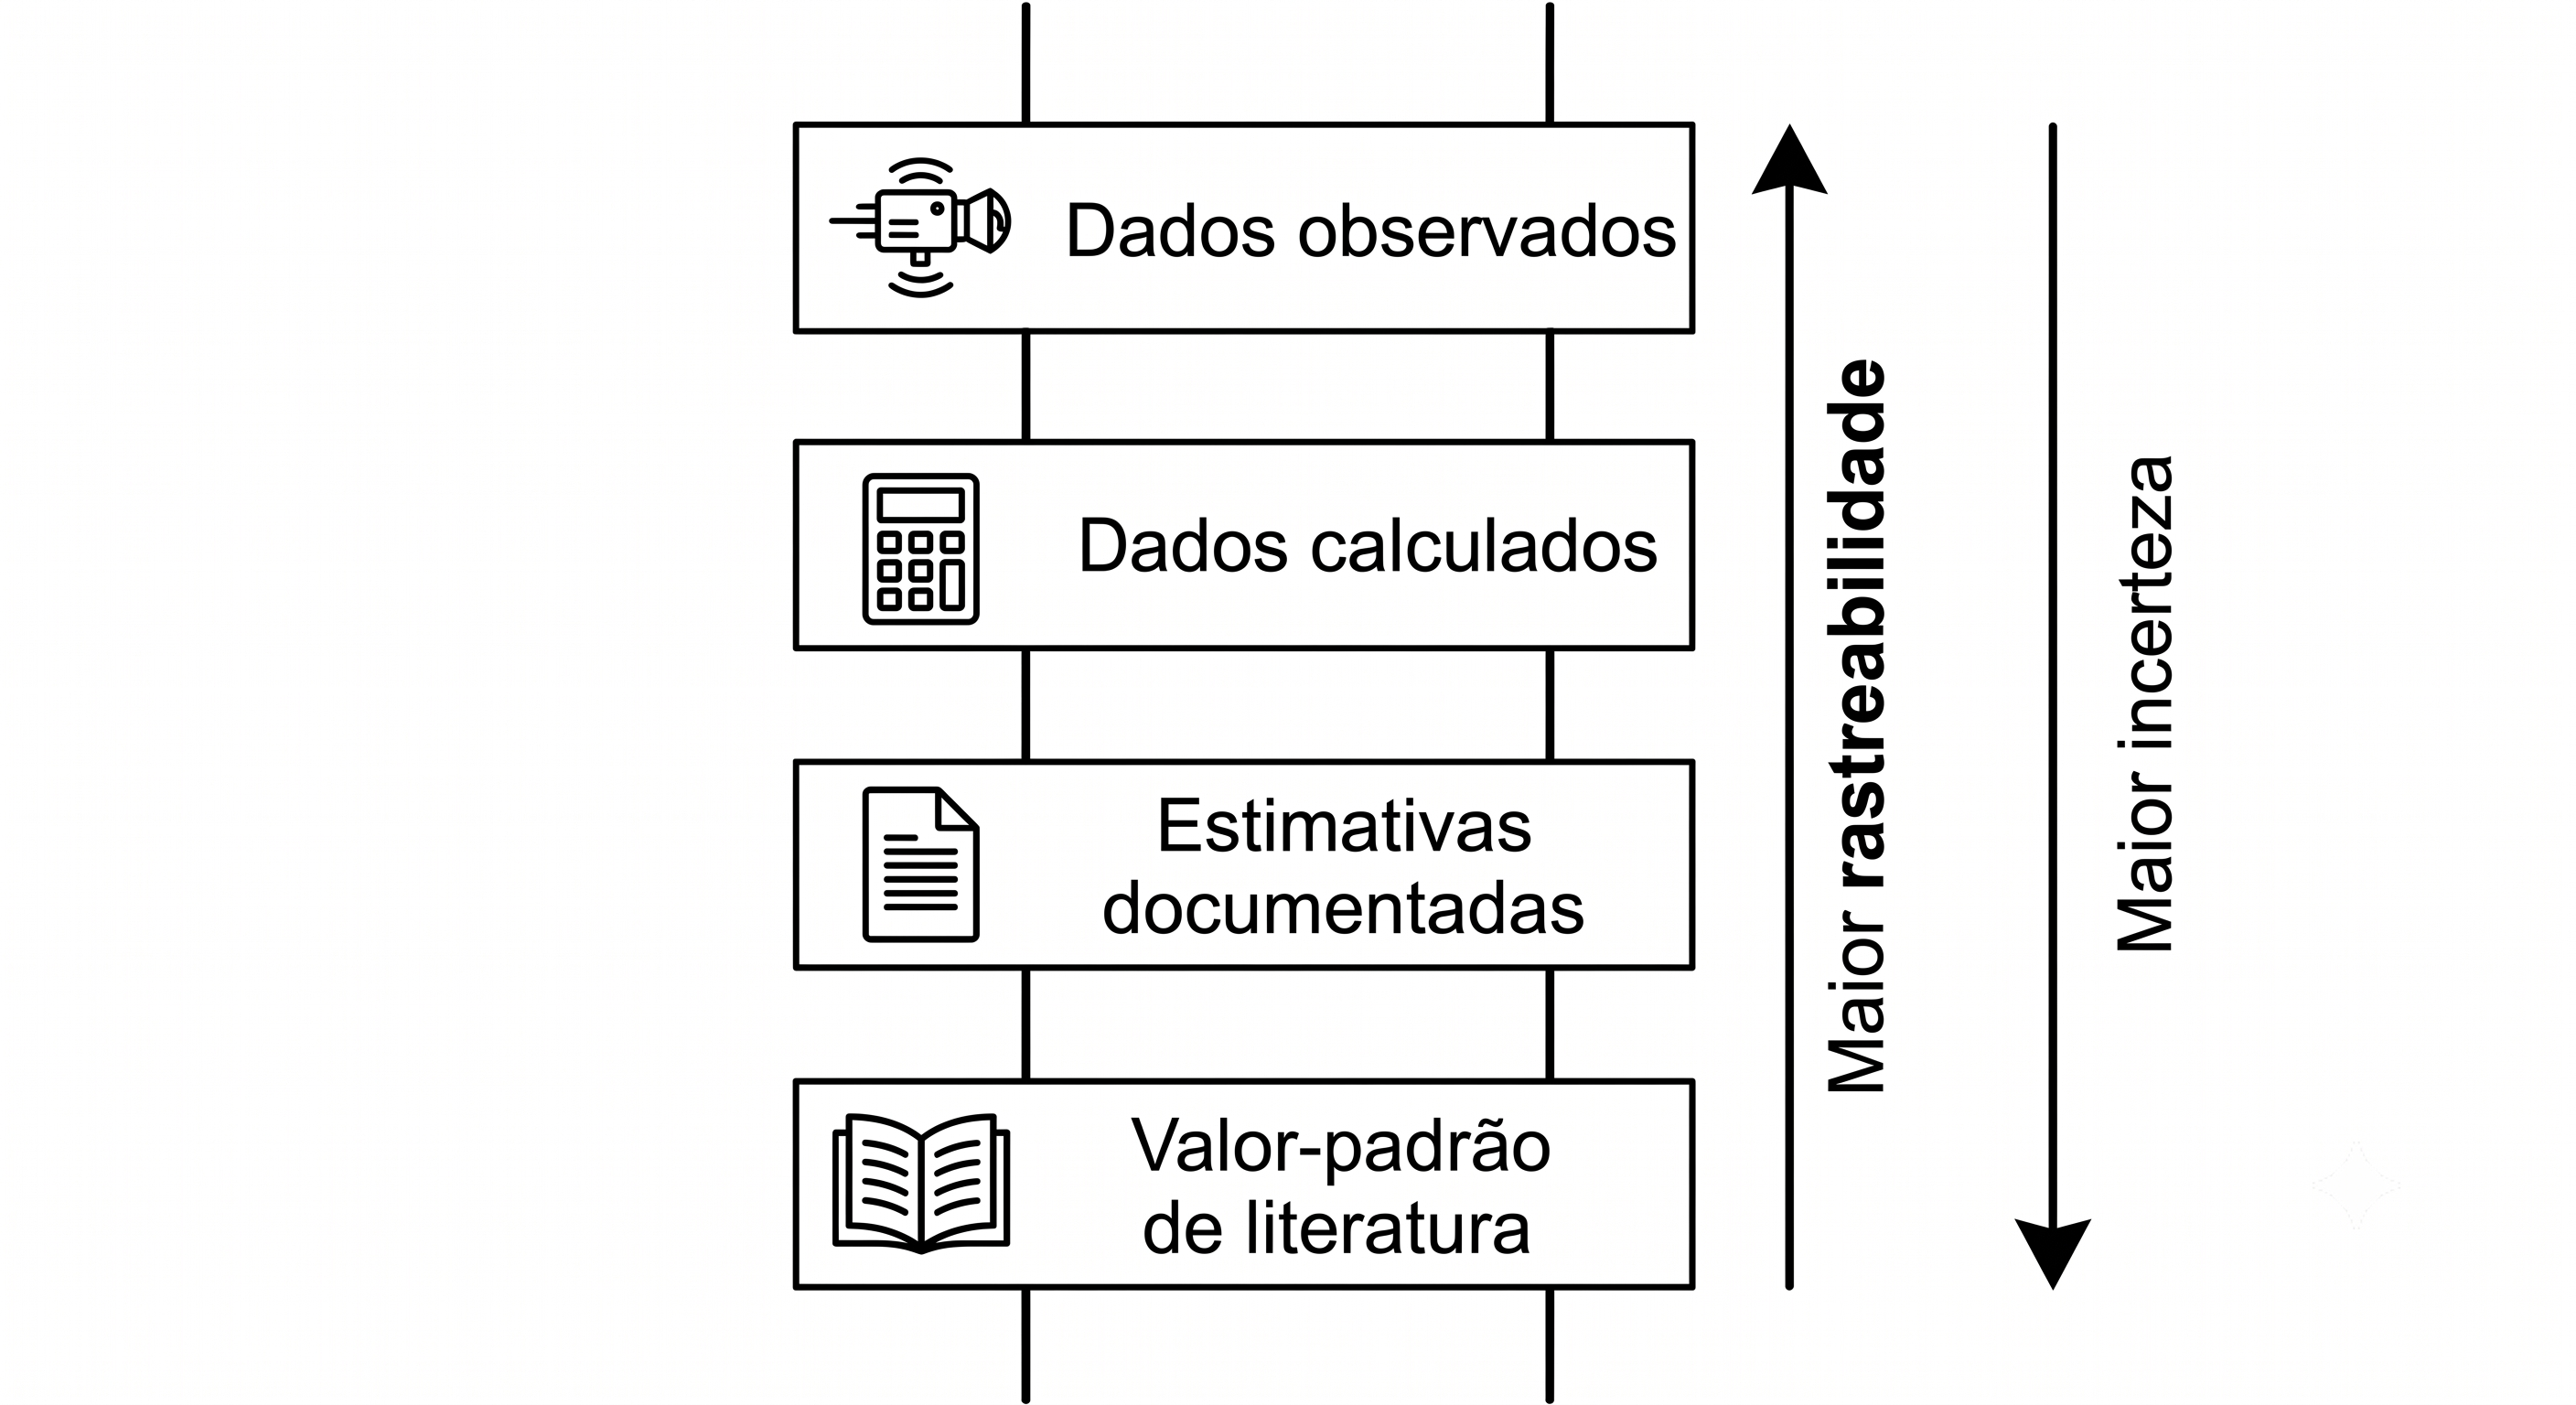
\includegraphics[width=0.85\textwidth]{images/figura_A_1.png}
\caption{Hierarquia de proveniência adotada para classificação das fontes de dados, priorizando maior rastreabilidade e explicitando o aumento de incerteza associado a estimativas e valores-padrão de literatura.}
\label{fig:proveniencia-hierarquia}
\end{figure}

A Tabela~\ref{tab:app-proveniencia-distancias} detalha a hierarquia aplicada às distâncias e aos componentes de rota. A leitura mais forte depende de referência específica para o par e para a fronteira analisada; a leitura mais fraca deve permanecer como triagem, lacuna ou sensibilidade.

\begin{table}[htbp]
\centering
\small
\caption{Hierarquia de proveniência para distâncias e componentes de rota.}
\label{tab:app-proveniencia-distancias}
\begin{tabularx}{\textwidth}{L{0.24\textwidth}Y Y}
\toprule
Proveniência & Uso metodológico & Limite de interpretação \\
\midrule
Roteamento rodoviário/cache & Distância terrestre para rota direta, \emph{pre-carriage} e \emph{on-carriage}. & Não é trajetória GPS medida nem rota comercial efetivamente usada.\\
\codecell{seamatrix} & Distância marítima matricial para par de portos aplicável. & Não comprova escala, frequência, serviço ou contrato.\\
\codecell{external\_reference} & Referência documentada para o par de portos do cenário. & Só vale para o par e a unidade informados.\\
\codecell{manual\_override} & Substituição documentada ou entrada forçada para cenário rastreado. & Deve permanecer explícita como decisão metodológica.\\
\codecell{haversine\_fallback} & Aproximação geométrica quando falta fonte melhor. & Triagem; não valida rota marítima operacional.\\
\codecell{unavailable} & Ausência de valor defensável. & Não deve ser tratado como zero silencioso.\\
\bottomrule
\end{tabularx}
\end{table}

\section{Operações portuárias e hoteling}
\label{sec:app-portops-hoteling}

Operações portuárias e \emph{hoteling} têm importância metodológica porque a alternativa multimodal não é apenas uma perna marítima. Quando o cenário aplica a intensidade EU MRV por trabalho de transporte, o indicador anual é tratado como abrangente do consumo reportado pelo navio e o \emph{hoteling} não é somado separadamente, evitando dupla contagem. A Tabela~\ref{tab:app-portops-proveniencia} registra a regra de interpretação para os componentes representados separadamente e para os níveis de proveniência usados nesses componentes.

\begin{table}[htbp]
\centering
\small
\caption{Proveniência de operações portuárias e hoteling.}
\label{tab:app-portops-proveniencia}
\begin{tabularx}{\textwidth}{L{0.25\textwidth}Y Y}
\toprule
Proveniência & Uso permitido & Cautela \\
\midrule
\codecell{observed} & Usar como dado observado para porto, chamada ou condição documentada. & Ainda não equivale a inventário terminal-específico completo.\\
\codecell{estimated\_port\_average} & Usar como média ponderada quando observações específicas sustentam a estimativa. & Menor confiança que observação direta do caso.\\
\codecell{literature\_default} & Usar como padrão documentado quando não há valor observado defensável. & Deve ser identificado como aproximação.\\
\codecell{unavailable} & Registrar ausência de dado. & Não converter ausência em zero emissões, zero custo ou zero tempo.\\
\bottomrule
\end{tabularx}
\end{table}

\chapter{Validação, benchmark e evidências complementares}
\label{app:validacao}

Este apêndice reúne os controles usados para auditar o cálculo marítimo e interpretar os benchmarks do \CabotageLens{}. Os números apresentados correspondem aos artefatos rastreados e permanecem vinculados à fonte, à unidade e à regra de agregação descritas no Capítulo~\ref{ch:validacao}.

\section{Fluxo de classificação da evidência}
\label{sec:app-mapa-validacao}

A Figura~\ref{fig:fluxo-classificacao-evidencia} mostra a passagem entre definição do cenário, execução, verificação da proveniência e classificação de uso. A disponibilidade de um resultado numérico não substitui a análise de sua fronteira.

\begin{figure}[htbp]
\centering
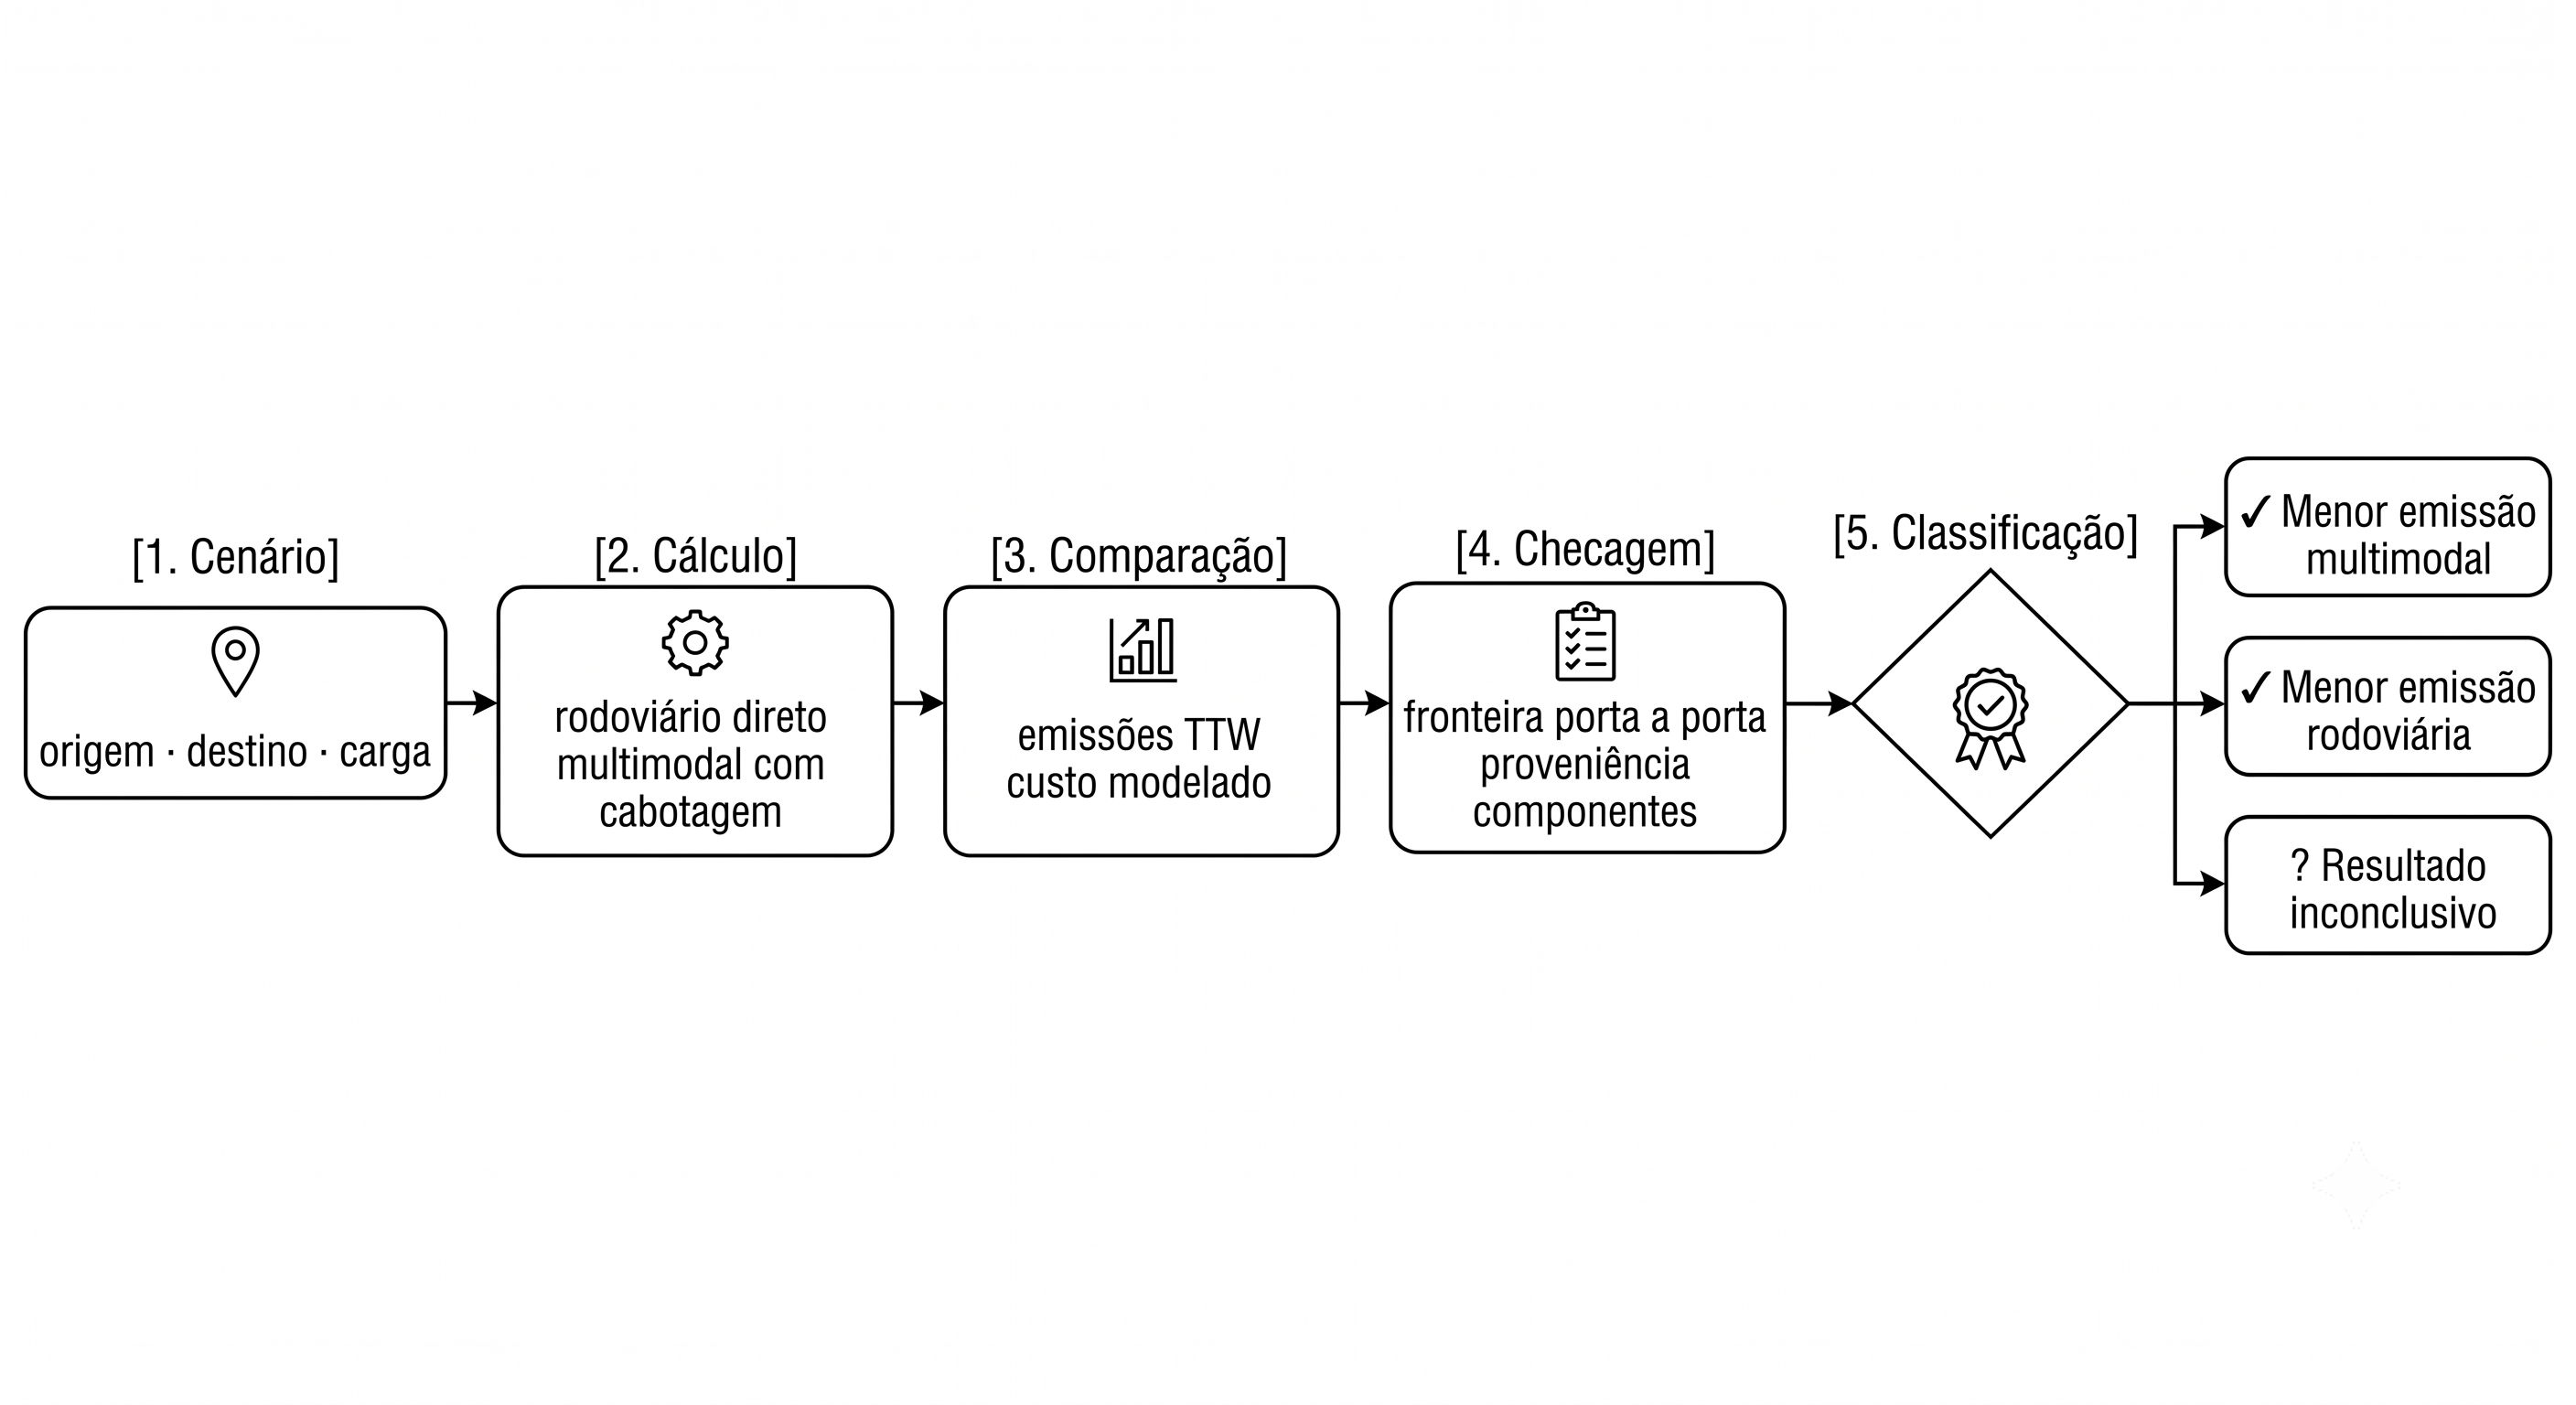
\includegraphics[width=0.95\textwidth]{images/figura_B_1.png}
\caption{Fluxo de classificação de evidências utilizado para organizar cada cenário avaliado.}
\label{fig:fluxo-classificacao-evidencia}
\end{figure}

\begin{table}[htbp]
\centering
\small
\caption{Perguntas de auditoria associadas às camadas de evidência.}
\label{tab:app-camadas-evidencia}
\begin{tabularx}{\textwidth}{L{0.26\textwidth}Y Y}
\toprule
Camada & Pergunta de auditoria & Registro esperado \\
\midrule
Dados ANTAQ & A sequência pertence à mesma viagem e a origem antecede o destino? & Identificador da viagem, ordem das escalas, movimentos de carga e cadeia completa de portos.\\
Intensidade MRV & O valor foi associado pelo IMO ou resolvido por fallback? & Fonte, ano, tipo ou classe, estatística robusta e tamanho da amostra.\\
Atividade da viagem & A carga a bordo e a distância foram aplicadas a cada subtrecho? & Massa, milhas náuticas, trabalho de transporte e combustível por subtrecho.\\
Agregação do par & Todas as viagens elegíveis contribuíram uma vez? & Contagens, pesos, mediana ponderada, regra de empate e tratamento de peso zero.\\
Geometria da rota & O caminho é uma sequência observada e contínua? & Portos, viagem candidata, critério de seleção e fontes de distância.\\
Resultado multimodal & As pernas usam a mesma unidade funcional e fronteira? & Carga do cenário, componentes rodoviários, marítimos e portuários, custo e emissões.\\
\bottomrule
\end{tabularx}
\end{table}

\section{Controles do artefato marítimo}
\label{sec:app-controles-artefato}

O arquivo direcional registra a versão de esquema, a data de geração, a hierarquia de intensidade, a política de outliers, o critério de seleção de corredor e os contadores de cobertura. A Tabela~\ref{tab:app-controles-artefato} consolida os campos que permitem rejeitar um artefato incompleto ou interpretar sua composição.

\begin{table}[htbp]
\centering
\footnotesize
\setlength{\tabcolsep}{4pt}
\renewcommand{\arraystretch}{1.15}
\caption{Controles de proveniência da matriz marítima direcional.}
\label{tab:app-controles-artefato}
\begin{tabularx}{\textwidth}{L{0.29\textwidth}L{0.27\textwidth}Y}
\toprule
Controle & Valor registrado & Função \\
\midrule
Esquema de intensidade & \codecell{maritime\_intensity\_schema\_version = 3} & Identifica a estrutura compatível com agregação por viagem--OD.\\
Modo de observação & \codecell{observed\_voyage\_corridors} & Restringe os caminhos a sequências completas de uma mesma viagem.\\
Escopo da intensidade & Todas as viagens elegíveis do mesmo par, em todos os corredores. & Define a população usada no estimador.\\
Estimador & Mediana ponderada por t$\cdot$nm. & Reduz a influência de intensidades extremas e preserva a atividade observada como peso.\\
Seleção do caminho & Ligação direta primeiro; depois, menor distância completa. & Separa geometria de rota e agregação estatística.\\
Reconstrução da carga & Deslocamento mínimo não negativo do prefixo acumulado. & Impede carga a bordo negativa e preserva movimentos observados.\\
Fallback de distância & Haversine para portos canônicos distintos sem valor positivo na matriz. & Mantém completude com fonte identificada.\\
Fallback de intensidade & Tipo com média aparada em 1\% por cauda ou mediana quando o corte não é possível; classe com média aparada do artefato ou mediana quando indisponível. & Explicita a estatística e a política de outliers.\\
\bottomrule
\end{tabularx}
\end{table}

\begin{table}[htbp]
\centering
\small
\caption{Contadores de cobertura preservados no artefato marítimo.}
\label{tab:app-contadores-maritimos}
\begin{tabularx}{\textwidth}{Y r Y}
\toprule
Contador & Valor & Observação \\
\midrule
Viagens / paradas / chamadas portuárias & \num{1324} / \num{6797} / \num{7103} & Estrutura observacional da ANTAQ.\\
IMOs ANTAQ / IMOs associados ao MRV & \num{389} / \num{243} & Cobertura de intensidade específica.\\
Subtrechos brutos / calculados & \num{5473} / \num{5438} & Diferença explicada por aliases consecutivos contraídos.\\
Distância da matriz / haversine & \num{5023} / \num{415} & Proveniência da distância por subtrecho.\\
Intensidade IMO / fallback & \num{3290} / \num{2148} & Proveniência da intensidade por subtrecho.\\
Observações viagem--OD / pares direcionados & \num{12025} / \num{177} & Base da agregação por origem--destino.\\
\bottomrule
\end{tabularx}
\end{table}

\section{Exemplo completo de auditoria: Santos--Manaus}
\label{sec:app-santos-manaus}

Para Santos--Manaus, a população estatística reúne \num{89} observações viagem--OD distribuídas em \num{22} corredores. Cada observação soma todos os seus subtrechos entre os dois portos e contribui uma única vez para a distribuição do par. A Tabela~\ref{tab:app-santos-manaus} permite conferir a separação entre a intensidade representativa e o caminho utilizado no cenário.

\begin{table}[htbp]
\centering
\small
\caption{Proveniência do par Porto de Santos--Porto de Manaus.}
\label{tab:app-santos-manaus}
\begin{tabularx}{\textwidth}{L{0.37\textwidth}Y}
\toprule
Campo & Valor \\
\midrule
Viagens resolvidas com trabalho positivo & \num{89} \\
Corredores completos observados & \num{22} \\
Observações com IMO exato & \num{40} \\
Observações com fallback de tipo & \num{49} \\
Participação do fallback no trabalho de transporte & \num{59.54}\% \\
Intensidade representativa & \num{9.322050} g/(t$\cdot$nm) \\
Método & Mediana inferior ponderada pelo trabalho de transporte \\
Caminho selecionado & Porto de Santos--Porto de Manaus \\
Critério do caminho & Ligação direta observada \\
Distância selecionada & \num{6112} km \\
\bottomrule
\end{tabularx}
\end{table}

A presença de uma ligação direta determina apenas o caminho. As viagens que passam por Itajaí, Paranaguá, Salvador, Suape, Pecém, Vila do Conde e outros portos permanecem na população estatística quando formam uma cadeia completa em que Santos antecede Manaus. O cálculo utiliza, portanto, a diversidade observada de corredores sem impor uma sequência portuária única.

\section{Fronteira de operações portuárias e \emph{hoteling}}
\label{sec:app-nota-portops-hoteling}

Quando o consumo marítimo é calculado com a intensidade MRV por trabalho de transporte, o indicador anual é tratado como abrangente do consumo reportado da embarcação para a fronteira considerada. O \emph{hoteling} não é somado separadamente nesse modo, reduzindo o risco de dupla contagem. As operações portuárias permanecem componentes explícitos quando possuem fonte identificada. Valores observados, médias de portos observados, padrões documentados e indisponibilidade são categorias distintas de proveniência; uma ausência não é convertida em zero de atividade.

\section{Benchmark externo}
\label{sec:app-benchmark}

\begin{table}[htbp]
\centering
\small
\caption{Resumo do benchmark externo associado aos estudos de Gustavo Costa.}
\label{tab:app-benchmark-resumo}
\begin{tabularx}{\textwidth}{L{0.40\textwidth}r Y}
\toprule
Item & Valor & Interpretação \\
\midrule
Células de matriz parseadas & \num{36} & Inventário total lido pelo roteiro de comparação.\\
Pares positivos e suportados & \num{21} & Denominador da comparação direcional.\\
Pares não comparáveis & \num{15} & Seis pares iguais e nove linhas rodoviárias nulas ou não positivas.\\
Acordo direcional & 21/21 & As duas fontes favorecem a alternativa com cabotagem em emissões.\\
Classificação & \codecell{same\_direction\_large\_gap} & Apoio ao sinal modal, sem equivalência de magnitude.\\
\bottomrule
\end{tabularx}
\end{table}

A comparação preserva as diferenças de distância, carga, portos, alocação, fatores e fronteira ambiental. Seus parâmetros permanecem separados dos parâmetros operacionais do aplicativo; o benchmark apoia a leitura do sinal modal, mas não calibra a intensidade marítima nem a magnitude dos resultados.

\section{Categorias de uso}
\label{sec:app-categorias-uso}

A Tabela~\ref{tab:app-categorias-uso} resume as categorias utilizadas para controlar afirmações. Ela complementa a Tabela~\ref{tab:categorias-uso}.

\begin{table}[htbp]
\centering
\footnotesize
\setlength{\tabcolsep}{4pt}
\renewcommand{\arraystretch}{1.15}
\caption{Resumo operacional das categorias de evidência.}
\label{tab:app-categorias-uso}
\begin{tabularx}{\textwidth}{L{0.35\textwidth}Y}
\toprule
Categoria & Leitura permitida \\
\midrule
\codecell{headline\_candidate} & Resultado principal somente com rota, fonte, unidade e fronteira suficientes.\\
\codecell{sensitivity\_discussion} & Comportamento condicionado à premissa identificada.\\
\codecell{limitation\_example} / \codecell{excluded} & Exemplo de limite ou cenário fora da fronteira de uso.\\
\codecell{reference\_needed} / \codecell{methodology\_blocked} & Lacuna de fonte ou de decisão que impede conclusão quantitativa.\\
\codecell{benchmark\_supports\_direction} & Consistência direcional sem calibração de magnitude.\\
\codecell{benchmark\_boundary\_mismatch} / \codecell{not\_comparable} & Diferença de fronteira ou ausência de comparabilidade numérica.\\
\bottomrule
\end{tabularx}
\end{table}

\chapter{Checklist de reprodutibilidade}
\label{app:checklist-reprodutibilidade}

Este checklist orienta a repetição de uma análise. A reprodução não consiste apenas em obter o mesmo número. Também é necessário usar as mesmas fontes, unidades, regras de seleção e fronteiras. Ao final, outra pessoa deve conseguir explicar de onde veio cada parcela do resultado.

\section{Checklist técnico}
\label{sec:app-checklist-tecnico}

O primeiro passo é localizar os arquivos que definem o documento e a metodologia. A Tabela~\ref{tab:app-checklist-tecnico} indica onde cada parte fica registrada. Antes de executar uma análise, deve-se confirmar que o código, os dados processados e o relatório correspondem ao mesmo conjunto de regras.

\begin{table}[htbp]
\centering
\small
\caption{Checklist técnico de reprodutibilidade do relatório.}
\label{tab:app-checklist-tecnico}
\begin{tabularx}{\textwidth}{L{0.25\textwidth}L{0.32\textwidth}Y}
\toprule
Item & Onde conferir & O que deve ser verificado \\
\midrule
Documento principal & \texttt{docs/report/main.tex} & Ordem dos capítulos, apêndices e base bibliográfica. \\
Capítulos modulares & \texttt{docs/report/chapters/} & Texto da metodologia, implementação, resultados e limites. \\
Apêndices de suporte & \texttt{docs/report/appendices/} & Parâmetros, auditorias e checklists usados para explicar a execução. \\
Figuras e diagramas & \texttt{docs/report/images/} & Correspondência entre a imagem, a legenda e a regra descrita no texto. \\
Tabelas e matrizes & Ambientes \texttt{tabular}, \texttt{tabularx} e \texttt{longtable} & Unidade, fonte e significado de cada indicador quantitativo. \\
Base bibliográfica & \texttt{docs/references.bib} & Existência das referências citadas e compatibilidade com a afirmação. \\
\bottomrule
\end{tabularx}
\end{table}

\section{Sequência recomendada de reprodução}

Uma execução pode ser conferida em seis passos:

\begin{enumerate}
    \item Fixar origem, destino e massa da carga.
    \item Registrar os portos escolhidos e as distâncias rodoviárias.
    \item Listar as viagens ANTAQ em que a origem marítima aparece antes do destino marítimo.
    \item Conferir carga a bordo, distância, trabalho de transporte e fonte da intensidade em cada viagem.
    \item Recalcular a mediana ponderada e, separadamente, conferir o caminho geométrico selecionado.
    \item Somar as pernas representadas e verificar se a saída continua dentro das fronteiras \ttw{} e de custo modelado.
\end{enumerate}

Em Santos--Manaus, essa sequência deve recuperar 89 observações em 22 corredores, sendo 40 por IMO e 49 por fallback. A participação do fallback deve ser 59,54\% do trabalho de transporte. A intensidade aplicada deve ser 9,322050~g/(t$\cdot$nm), e a média diagnóstica, 25,243618~g/(t$\cdot$nm). O caminho deve ser a ligação direta de 6.112~km ou 3.300,216~nm.

Se a massa de teste for 14~t, a verificação manual da parcela de navegação deve produzir:

\begin{equation}
9{,}322050\times14\times3.300{,}216/1000
= 430{,}71~\text{kg de combustível}.
\end{equation}

Somente a massa de 14~t é uma entrada ilustrativa. Os indicadores do par e o caminho são dados da execução atual. O valor de 430,71~kg não inclui toda a cadeia porta a porta.

\section{Checklist metodológico}
\label{sec:app-checklist-metodologico}

A Tabela~\ref{tab:app-checklist-metodologico} deve ser usada como uma lista de confirmação. Cada linha responde ``sim'' ou ``não'' para uma condição necessária. Se uma condição não for atendida, o resultado precisa ser corrigido, classificado como limitação ou excluído da comparação quantitativa.

\begingroup
\footnotesize
\setlength{\LTleft}{0pt}
\setlength{\LTright}{0pt}
\setlength{\tabcolsep}{4pt}
\renewcommand{\arraystretch}{1.10}
\begin{longtable}{L{0.29\textwidth}L{0.65\textwidth}}
\caption{Checklist de consistência metodológica do framework.}
\label{tab:app-checklist-metodologico}\\
\toprule
Dimensão de controle & Pergunta de verificação \\
\midrule
\endfirsthead
\toprule
Dimensão de controle & Pergunta de verificação \\
\midrule
\endhead
Comparação porta a porta & A origem, o destino e a massa são iguais na rodovia direta e na cadeia multimodal? \\
Fronteira ambiental & O resultado está identificado como emissão operacional \ttw{} de \cooe{}, sem ser confundido com \wtw{} ou LCA? \\
Fronteira econômica & O valor está identificado como custo operacional modelado, e não como frete ou tarifa? \\
Sequência das viagens ANTAQ & Todas as escalas pertencem à mesma viagem, com a origem antes do destino? \\
Cobertura de corredores & Ligações diretas e multiescala foram consideradas, com uma contribuição por viagem e par? \\
Carga a bordo & Embarques e desembarques foram acumulados e a carga permaneceu não negativa? \\
Trabalho de transporte & Foram somados carga a bordo vezes distância de todos os subtrechos do OD? \\
Intensidade marítima & O sistema procurou primeiro o IMO no EU MRV e registrou qualquer fallback por classe ou tipo? \\
Outliers do fallback & O tipo usou média aparada de 1\% ou mediana; a classe usou média aparada ou mediana; e o IMO exato foi preservado? \\
Agregação do par & A intensidade é a mediana inferior ponderada pelo trabalho de transporte de todas as viagens e corredores elegíveis? \\
Pesos nulos & Pesos nulos foram excluídos quando havia peso positivo e tratados por mediana não ponderada quando todos eram nulos? \\
Seleção de caminho & Foi escolhida uma ligação direta observada ou, na sua ausência, a menor cadeia completa, sem combinar viagens? \\
Proveniência de distâncias & Cada perna informa se veio de matriz, API, referência, fallback ou override? \\
Componentes portuários & As operações portuárias têm fonte e o \emph{hoteling} não foi duplicado quando se usou intensidade MRV abrangente? \\
Tratamento de dados ausentes & Dados indisponíveis permaneceram como lacuna, em vez de serem transformados em zero? \\
Compatibilidade do artefato & A matriz informa schema, data, política de intensidade, regra de caminho e cobertura? \\
Classificação de evidência & O resultado foi limitado à sua categoria, sem alegação de superioridade universal? \\
\bottomrule
\end{longtable}
\endgroup

Ao concluir o checklist, o leitor deve conseguir repetir a fórmula e também explicar seus limites. No exemplo de 14~t, isso significa reproduzir os 430,71~kg de navegação e declarar que o número não é emissão \wtw{}, custo comercial ou confirmação de serviço.


% O estilo ABNT/USP e a revisão completa de metadados bibliográficos ficam
% para a etapa final; os campos internos note/file são suprimidos na renderização.
\printbibliography[title={Referências}]

\end{document}
